\chapter{相关技术研究}
\label{chap:chapter02}
上一章的内容中详细描述了本研究课题的研究背景,并且进一步分析了国内外的相关研究进展和现状,最后提出了本课题说研究的三个主要数据源和预计采用的研究方法。依据研究对象不同讲课题研究分为三个主要部分。本章将会详细的分析和阐述一些针对感知数据预处理的关键技术和方法以及论文中所涉及的快速语义轨迹计算、缺失轨迹补全等算法。
\section{用户轨迹预处理}
\label{sec:section2-1}
在用户的轨迹信息的采集过程中,因受到地形、气候、GPS传感器和SA干扰误差的影响,会导致用户位置的跳跃移动等称之为“GPS漂移现象”\upcite{wegmann2002image},GPS的位置漂移使得用户的轨迹数据中存在大量的噪音数据,影响后续对数据的处理和分析。因此对采集到的用户轨迹数据采取滤波处理,消除轨迹中所蕴含的噪音数据。GPS位置的采集还受到地形环境的影响,在室内无法获取GPS位置信息的时候会导致用户轨迹的缺失,一旦用户轨迹出现缺失,对后续的度量工作也会产生影响。因此本小节首先描述GPS轨迹的噪音消除算法以及我们所采用的轨迹补全算法,最后描述各种常用聚类算法。
\subsection{滤波算法}
\label{sec:section2-1-1}
滤波的主要目的是消除特定频率波段的噪音,用户的日常运动是连续的,所以采集到的用户GPS轨迹数据㛑也应该是由连续的位置点构成的,但是由于GPS采集过程中受到漂移现象的影响,导致用户的GPS轨迹中存在位置点跳跃现象,因此要通过采用滤波算法对用户轨迹进行异常点剔除工作。接下来主要描述了一些经常使用的滤波算法:均值滤波、中值滤波、卡尔曼滤波这三种滤波算法。
\par a)均值滤波:均值滤波也被称之为线性滤波,主要思想是采用结合中心点周围的数值,采取邻域平均法来表示这个邻域。数学公式表示如\ref{equ:chap2:meanFilter}所示,假设当前点为$p$,则设置点$p$为采样中心。将$p$前$m$个采样点和后$m$个采样点的平均值作为当前点$p$的取值。
\begin{equation}
\label{equ:chap2:meanFilter}
g(p)=\frac{1}{2m} \ast \sum_{j=i-m,j\neq i}^{i+m}g(j)
\end{equation}
\par b)中值滤波:中值滤波是一种基于排序统计理论的提出信号噪声点的非线性的信号处理方法,其基本原理就是点$p$的取值是由其邻域内各个点取值的中值来决定的,让数据能够更加接近于真实的取值,从而有效地减少噪声数据点。中值滤波的具体数学公式见\ref{equ:chap2:medianFilter},其中函数$median()$表示求中值。
\begin{equation}
\label{equ:chap2:medianFilter}
g(p)=median({g(p-m),...,g(p-1),g(p),g(p+1),...,g(p+m)})
\end{equation}
\par c)卡尔曼滤波:卡尔曼滤波是卡尔曼于1960年提出的\upcite{kalman1960new},卡尔曼滤波器由一系列递归数学公式描述。它们提供了一种高效可计算的方法来估计过程的状态,并使估计均方误差最小。卡尔曼滤波
器应用广泛且功能强大:它可以估计信号的过去和当前状态,甚至能估计将来的状态,即使并不知道模型的确切性质。接下来将介绍卡尔曼理论和实用方法。
%--------------------------------------------------------------
\par 在此之前需要引入离散随机过程,卡尔曼滤波器用于估计离散时间过程的状态变量$x\in \Re^{n}$,这个离散随机过程的方程如\ref{equ:chap2:kalman-01}描述:
\begin{equation}
\label{equ:chap2:kalman-01}
x_{k}=Ax_{k-1}+Bu_{k-1}+w_{k-1}
\end{equation}
\par 定义我们所观测到的变量$x\in \Re^{m}$,在此基础上得到卡尔曼滤波的测量方程见公式\ref{equ:chap2:kalman-02}:
\begin{equation}
\label{equ:chap2:kalman-02}
z_{k}=Hx_{k}+v_{k}
\end{equation}

\par 其中随机的变量$w_{k}$和$v_{k}$分别表示计算过程中的激励噪声和观测到的噪声,我们假设他们二者之间相互独立,则可以得到正太分布的白色噪声如公式\ref{equ:chap2:kalman-03}和\ref{equ:chap2:kalman-04} 描述:
\begin{equation}
\label{equ:chap2:kalman-03}
  p(w)\sim N(0,Q)
\end{equation}
\begin{equation}
\label{equ:chap2:kalman-04}
  p(v)\sim N(0,R)
\end{equation}
\par 在实际随机过程中,激励噪声$w_{k}$的协方差矩阵$Q$和观测到的噪声$v_{k}$的协方差矩阵$R$是会随着每次迭代计算而改变的,因此为了便于推演我们假设它们都是固定的常数。当函数$u_{k-1}$等于0时或者噪声函数$w_{k-1}$等于0时,随机过程方程\ref{equ:chap2:kalman-01}中的$n*n$阶矩阵$A$将$k-1$时刻的状态通过线性映射到$k$时刻的状态,$n*l$阶矩阵$B$表示变量$u\in \Re^{l}$的增益,为了便于计算,这些变量在此都假设为常数。
\par 我们定义$\hat{x}_{\bar{k}} \in \Re^{n}$为在第$k$项之前的状态下计算得到的第$k$项的先验状态估计值,设$\hat{x}_{k} \in \Re^{n}$表示已经得到的变量$z_{k}$ 时,第k步的后验状态估计值。由此根据以上描述我们可以定义出如\ref{equ:chap2:kalman-05}和\ref{equ:chap2:kalman-06}说表示的先验估计误差后后验估计误差:
\begin{equation}
\label{equ:chap2:kalman-05}
  e_{\bar{k}}\equiv x_{k}-\hat{x}_{\bar{k}}
\end{equation}
\begin{equation}
\label{equ:chap2:kalman-06}
  e_{k}\equiv x_{k}-\hat{x}_{k}
\end{equation}
\par 进一步得出先验估计和后验估计的协方差为:
\begin{equation}
\label{equ:chap2:kalman-07}
P_{\bar{k}}=E\left [ e_{\bar{k}} {e_{\bar{k}}}^{T}  \right ]
\end{equation}
\begin{equation}
\label{equ:chap2:kalman-08}
P_{k}=E\left [ e_{k} {e_{k}}^{T}  \right ]
\end{equation}
\par 基于以上的理论准备,构建出卡尔曼滤波算法的数学表达式\ref{equ:chap2:kalman-09},其含义为:先验估计$\hat{x}_{\bar{k}}$和测量得到的变量$z_{k}$ 同其预测值$H\hat{x}_{\bar{k}}$之差的线性组合共同组成了后验状态估计$\hat{x}_{x}$
\begin{equation}
\label{equ:chap2:kalman-09}
\hat{x}_{k}=\hat{x}_{\bar{k}} + K(z_{k}-H\hat{x}_{\bar{k}})
\end{equation}
\par 根据\ref{equ:chap2:kalman-09}中表示可以进一步得到$K$的具体表达公式,其中真实变量与其预测之差$(z_{k}-H\hat{x}_{\bar{k}})$被称之为残差,该指标有效地反映了预测值与实际值之间的不一致的程度,如果残差为零,则表示二者完全相吻合。$n*m$阶矩阵$K$称之为剩余增益或者混系数,其主要作用是使得\ref{equ:chap2:kalman-08}中所得到的后验估计误差协方差最小,其计算步骤为:首先根据\ref{equ:chap2:kalman-09} 代入\ref{equ:chap2:kalman-06}中求得$e_{k}$,再将$e_{k}$代入\ref{equ:chap2:kalman-08}求得期望后对$K$进行求导,并令一阶导数为零就可以求得$K$的值如\ref{equ:chap2:kalman-10}:
\begin{align}
\label{equ:chap2:kalman-10}
\hat{x}_{k}=\hat{x}_{\bar{k}} + K(z_{k}-H\hat{x}_{\bar{k}})
\nonumber \\
=\frac{P_{\bar{k}}H^{T}}{HP_{\bar{k}}H^{T}+R}
\end{align}
\par 从\ref{equ:chap2:kalman-10}中能够得知观测到的数据的噪音的协方差$R$越小,残余增益$K$越大,特别地当$R$趋向零时有:
\begin{equation}
\label{equ:chap2:kalman-11}
\lim_{P_{k} \to 0 }K_{k}=H^{-1}
\end{equation}
\par 另一方面,先验估计误差的协方差越小,残余增益$K$越小,特别当$P_{\bar{k}}$趋近于零时有:
\begin{equation}
\label{equ:chap2:kalman-12}
\lim_{P_{\bar{k}} \to 0 }K_{k}=0
\end{equation}
\par 综合\ref{equ:chap2:kalman-10}、\ref{equ:chap2:kalman-11}、\ref{equ:chap2:kalman-12}针对单个模型的测量利用上述说描述的所有公式就能够通过不断的迭代计算得出最优的估算结果。对于上述介绍的三种滤波技术而言,均值滤波在剔除数值中的随机噪音表现良好,但是不易消除脉冲误差;中值滤波能够减少偶然数据波动带来的误差影响,但是对变化快速的数据不宜使用;卡尔曼滤波最终的结果会优于前两者,但是模型较为复杂,所要求的运算时间复杂度也高于前面的滤波算法。
\subsection{轨迹停留点检测}
现实生活中用户的日常轨迹通常是有一系列包含了地理坐标和时间戳的GPS位置点构成,每个坐标点包含了详细的经纬度、时间戳信息、海拔高度、移动速度等信息。如图\ref{fig:2_1}所示。我们可以通过一些算法检测出用户在一段轨迹运动中停留过的地方称之为停留点\upcite{zheng2011computing},本文的停留点并不是指运动速度静止的点,而是由一系列GPS点构成的。如图\ref{fig:2_1}中$p_{4} \sim p_{8}$构成了一个停留点stay point在图中由红色点表示。这个点表示用户在该区域内的停留时间超过了一个设定的时间阈值$\Delta T$,相比于用户的其他轨迹位置点,这些计算得出的停留点蕴含了更重要的信息,通过语义标签甚至可以得出用户去过某家餐馆和电影院等。基于以上理论,用户的GPS位置轨迹可以转换为一组由停留点所组成的序列,如$sp_{1}\overset{\Delta_{t1}}{\rightarrow} sp_{2}\overset{\Delta_{t2}}{\rightarrow}\cdots \overset{\Delta_{tn-1}}{\rightarrow}sp_{n}$,这样由停留点所表示的序列不仅对原有数据维度进行了压缩,同时也保存了用户的重要信息。
\begin{figure}[H]
\centering
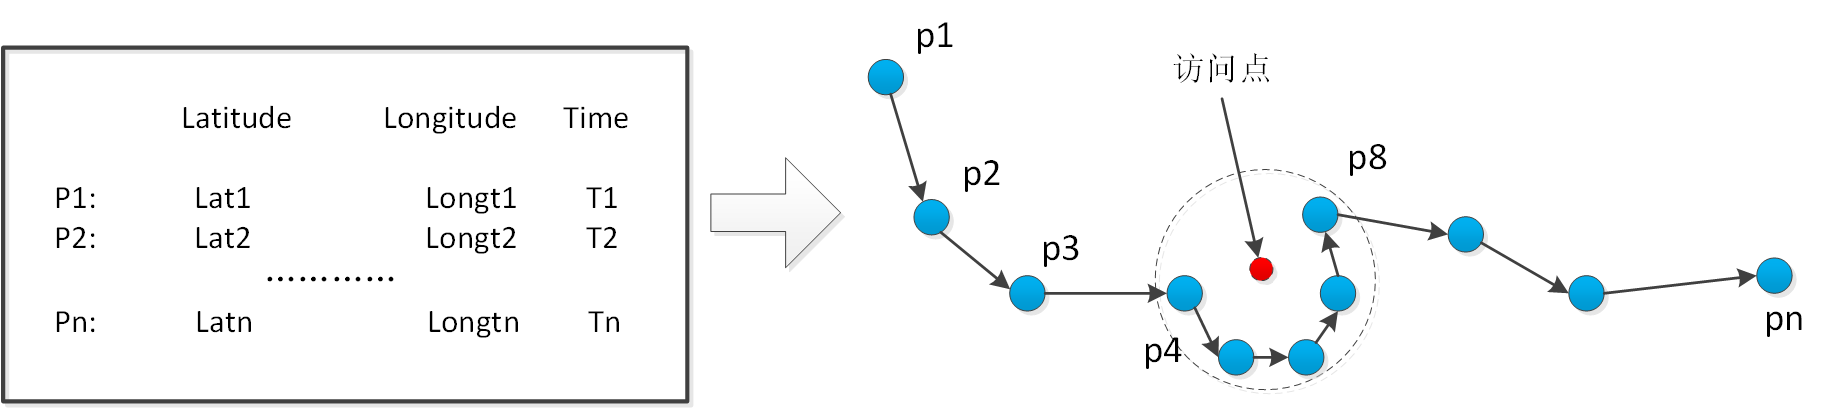
\includegraphics[width=0.8\textwidth]{figure2_1_gps}
\caption{用户GPS轨迹示例图}
\label{fig:2_1}
\end{figure}
\par 停留点的计算过程如\ref{alg2_1staypoint}所示。
\begin{algorithm}[htb]
\caption{停留点检测算法}
\label{alg2_1staypoint}
\begin{algorithmic}[1] %每行显示行号
				\REQUIRE 用户GPS轨迹 $Tra$,$\Delta T$,$\Delta_{distance}$
				\ENSURE 用户停留点序列$SP$
				%\Function {SPDec}{$Tra, \tau_{time},\tau_{distance}$}
				\STATE $i = 0$ , $PointNum= \left| \ Tra \right|$,$SP = Null$
				\WHILE {$i<PointNum$}
				\STATE $j = i+1$
				\WHILE {$j < PointNum$}
				\STATE $distance=Dis(Tra_{i},Tra_{j})$
				\IF {$distance > \Delta_{distance}$}
				\STATE $\Delta_{t}=Tra_{j}.T-Tra_{i}.T$
				\IF {$\Delta_{t} > \tau_{time}  $ }
				\STATE $p.Lat = avg(Tra_{k}.Lat)  $
				\STATE $p.Lng = avg(Tra_{k}.Lng)$
				\STATE $p.T = Tra_{i}.T(arv|lev)$%p.levT = Tra_{j}.T $
				\STATE $SP .add(p) ;j++; $
				\ENDIF				
				\ENDIF				
				\ENDWHILE
				\STATE $i=j ; break$
				\ENDWHILE
				\STATE \RETURN {$SP$}
				%\EndFunction				
\end{algorithmic}
\end{algorithm}
\subsection{聚类算法}
由于现实生活中人们可能会经常多次访问同一个空间地点,但是所计算得到的停留点却可能并不完全相同(坐标的变差,计算的误差等因素影响),因此采用传统直接比较停留点的方法不具备可行性。我们采取对停留点进行聚类的处理方法,这样地理位置非常相近的点就会被划分为同一个类别中。接下来介绍一些常用的聚类算法。
\par 聚类是属于无监督学习中的一种重要的方法,在其他的机器学习方法中如:回归分析、朴素贝叶斯网络等的数据都是带有类别标签$\gamma$,也就是说在训练集中的样例就已经给出了样例的类别,而聚类数据样本却没有给出样本类别$\gamma$聚类的目标是根据组内元素距离最小,组间距离最大将原始数据划分为若干组如图\ref{figure2_1cluster}所示。本节主要介绍几种常用的聚类分析方法:K-Means聚类算法、基于密度的DJ-Cluster 聚类算法以及近年发表的一种改进的基于密度的聚类算法。
\begin{figure}[htp]
\centering
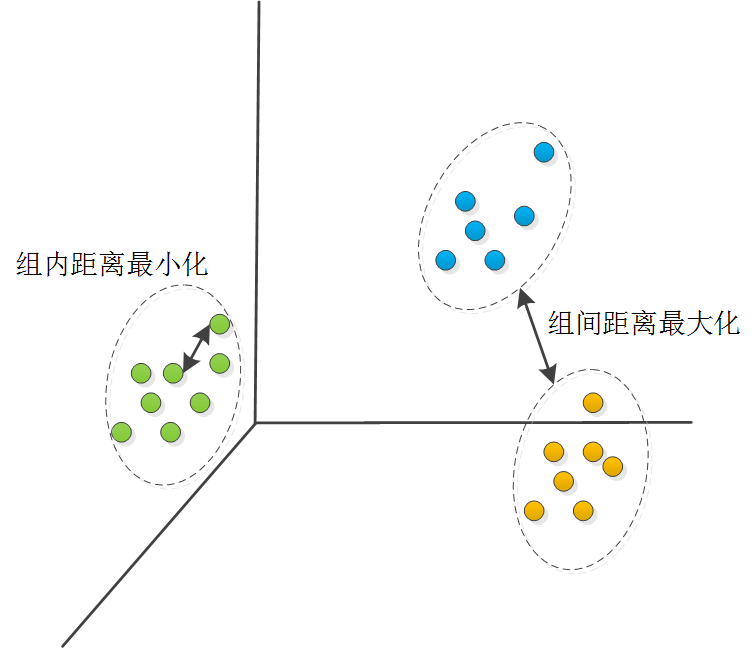
\includegraphics[width=0.8\textwidth]{figure2_1cluster}
\caption{聚类效果示意图}
\label{figure2_1cluster}
\end{figure}
\par  K-means聚类算法是比较经典的聚类方法之一,由J.MacQUEEN在1967提出\upcite{macqueen1967some}。该算法执行效率高,在大规模的数据处理聚类时被广泛使用,该算法输入$k$作为最终聚类的个数,将待分类的$n$个数据分成$k$个簇,使得簇内数据具有高的相似度而簇间的数据存在较低的相似度。K-means聚类算法的执行过程如下:首先根据输入的参数$k$随机从原始数据中选择$k$个对象,每个初始化的对象代表了一个簇的中心;其次,剩余的每个对象计算与簇中心的距离将它们赋予距离最近的簇;第一轮结束后将重新计算每个簇的中心,这个过程不断重复知道准则函数收敛或者簇没有新的变化为止,通常采用平方误差的度量准则如\ref{equ:chap2:k-means}:
\begin{equation}
\label{equ:chap2:k-means}
E=\sum_{i=1}^{k}\sum_{p\subset C}^{p}{\left | p-m_{i} \right |^{2}}
\end{equation}
\par K-means算法虽然简单,易于实现,但是在实际使用过程中需要用户指定$k$的取值,而$k$的取值是难以估计的,针对不同的数据事先并不可能确切的知道这些原始数据应该划分为多少个类别才正确;同时该聚类算法对异常数据非常敏感,一旦出现离群点将容易导致簇中心点出现漂移,对计算结果影响巨大。
%--------写到这里
\par 相比于前面描述的基于距离的聚类方法,研究者于2007年提出了一种基于密度的聚类算法DBSCAN\upcite{ester1996density}以及日后基于该算法改进的DJ-Cluster聚类算法\upcite{zhou2007discovering},DBSCAN算法的基本思想是扫描整个待分类的原始数据集,当扫描到数据对象P 时,计算P的$Eps$邻域内所密度可达的数据对象个数是否大于等于定义的$MinPts$,如果为真,则设立以P为核心的簇,然后尽可能的寻找与该簇密度相连的最大集合或者不断迭代查找该簇中每个数据对象的直接密度可达点,加入到该簇中。如图\ref{fig:figure2_2dbscan}中所示,设$MinPts=3$,从图中我们可以看出原始数据点M,P,O和点R的$Eps$邻域内说包含的点均大于等于$MinPts$因此都可以把它们标记为核心;M是P的直接密度可达,Q是M的直接密度可达。因此可以得知:Q是P的密度可达,但是P不是点Q的密度可达,点O,R和点S是密度相连的。通过实验证明,DBSCAN会受到$Eps$和$MinPts$取值的影响。
\begin{figure}[h]
\centering
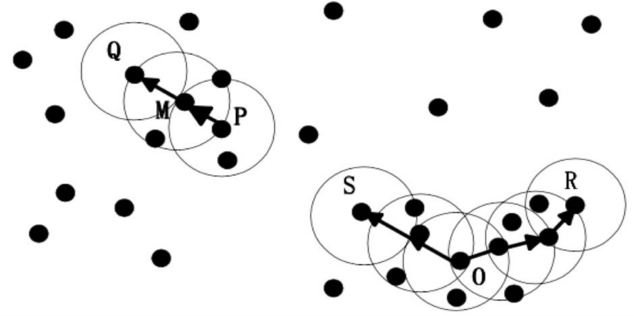
\includegraphics[width=0.8\textwidth]{figure2_2dbscan}
\caption{DBSCAN密度直达和密度可达示意图}
\label{fig:figure2_2dbscan}
\end{figure}
\par Rodriguez A等人2014年在Science上发表了一种新的基于密度的聚类算法\upcite{rodriguez2014clustering}。该算法相比较于之前的聚类算法,具有对参数不敏感便于输出正确的聚类结果的有点。该算法的主要改进想法是针对所有待聚类的组标点基于它们之间的距离,提出了两个新的标准属性:$\rho$和$\delta$,基于聚类中心点具有:中心点自身的密度大,即它的密度超过邻域集合点的密度同时距离其它密度大的中心点之间的距离也足够大这样的特征,其中局部密度$\rho$采用Cut-off kernel计算方式,公式如\ref{equ:chap2:Cut-off-kernel}所示,其中$p_{i}$表示S中与数据点$x_{i}$距离小于$d_{c}$的点的数量;$d_{c}$为截断距离需要用户事先设定并且保证$d_{c} >0$。
\begin{equation}
\label{equ:chap2:Cut-off-kernel}
\rho_{i}=\sum_{j \in I_{s}\setminus {i}}^{ }\chi (d_{ij}-d_{c})
\end{equation}
公式\ref{equ:chap2:Cut-off-kernel}中的$\chi(x)$的计算方式为:
\begin{equation}
\label{equ:chap2:chi-kernel}
\chi{x}=
\begin{cases}
1 & \mbox { $x<0$}\\
0 & \mbox { $x \geq  0$}
\end{cases}
\end{equation}
\par 算法中另一个指标距离$\delta$的定义为设$\left \{  q_{i} \right \}$表示$\left \{  p_{i} \right \}$的降序的下标序列,因此该序列满足:
\begin{equation}
\label{equ:chap2:se-delta}
\rho_{q_{1}} \geq \rho_{q_{2}} \cdots \geq \rho_{q_{N}}
\end{equation}
\par 则可根据公式\ref{equ:chap2:jisuan-delta} 计算出$\delta$:
\begin{equation}
\label{equ:chap2:jisuan-delta}
\chi{x}=
\begin{cases}
\underset{q_{j},j<i}{min} \left \{ d_{q_{i}q_{j}} \right \}  & \mbox { $i \geq 2$}\\
\underset{j\geq 2}{max} \left \{ \delta_{q_{j}} \right \} & \mbox { $i=1$}
\end{cases}
\end{equation}
该算法原理示意见图\ref{fig:2_3}和图\ref{fig:2_4},从图\ref{fig:2_4}可以看出,编号为1和编号为10的坐标点具有较大的$\rho$和$\delta$取值,因此在原始数据中我们将这两个点设置为簇的中心,而在图\ref{fig:2_3}中这两个坐标点恰好是分类簇的中心点;同时还出现了编号26-28三个“离群点”它们的特点是$\delta$值很大而$\rho$取值很小。
\begin{figure}[htp]
\centering
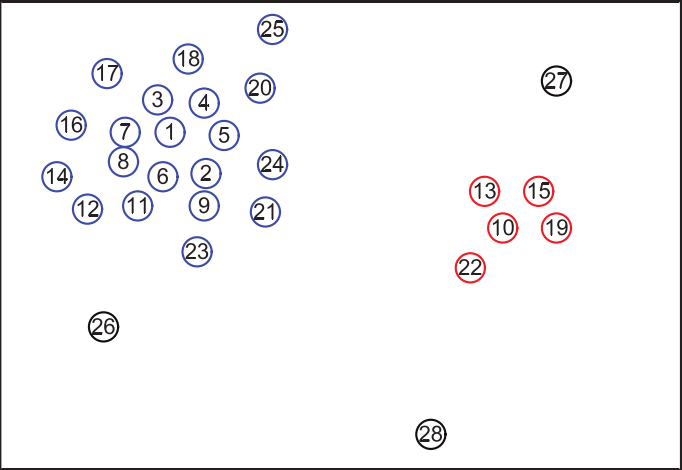
\includegraphics[width=4in]{figure2_3}
\caption{关于decision graph的示例\upcite{rodriguez2014clustering}}
\label{fig:2_3}
\end{figure}
\begin{figure}[htp]
\centering
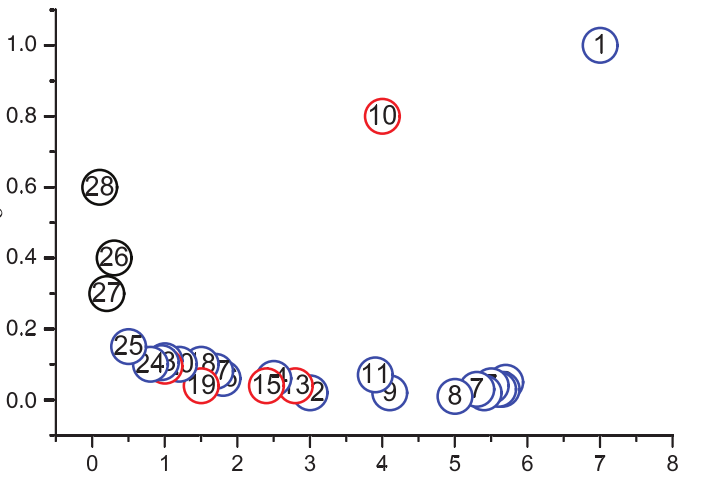
\includegraphics[width=4in]{figure2_4}
\caption{聚类中各点的$\rho$和$\delta$取值\upcite{rodriguez2014clustering}}
\label{fig:2_4}
\end{figure}
\par 总的来说,上述三种聚类算法通过精心调整参数都能取得非常好的聚类效果。不同的算法拥有不同的优缺点,在第四章我们将通过实验来展示各种算法在不同参数下的聚类结果。
\section{时间序列相似度度量方法}
\label{sec:section2-2}
我们阅读了大量社会心理学相关的论文书籍,从中证实得到在现实生活中关系亲密的两个用户会更加倾向于一起进行面对面的交流、共同进行社交活动等,因此通过对手机传感器数据的处理分析能够从中挖掘出人们现实生活中的关系强度。文献[37] 立足于空间距离,提出了在空间距离上非常接近的人们在现实生活中就越可能发生面对面的交互,该文献通过调研一个小区的住户发现人们在现实生活中越是接近,就越容易成为朋友。文献\cite{zajonc1968attitudinal}\cite{zillmann2000mood}进一步通过研究用户的轨迹数据发现由于在空间距离中接近的用户在现实生活中更可能产生交互行为,也就是说拥有相似日常生活轨迹的用户更可能产生交互活动。在现实生活中亦是如此,我们很容易和同自己经常出没同一个地点、行走在同一条轨迹上的人发展友谊关系。
\par 用户的轨迹序列由带有时间戳的位置数据构成,位置数据可能是GPS 也可能是基站号。因此我们可以将轨迹序列看作时间序列,从而使用一些时间序列相似度度量模型来度量轨迹的相似度,下面依次描述编辑距离和DTW这两种相似度度量方法以及序列熵值的计算方法。前面章节描述到用户的轨迹是由GPS位置点所构成的,包含了$(经度,纬度,时间戳)$等详细信息,因此我们将用户的轨迹看作一条由带有时间戳所构成的坐标点序列,采用序列相似度计算方式来处理轨迹之间的相似度。接下来详细描述两种常用的序列相似度计算方法。
\subsection{轨迹中心距离}
传统的计算序列相似度所采用的方法如:编辑距离、汉明距离和夹角余弦等有其优缺点,如果贸然用来计算用户轨迹序列的相似性可能不太符合实际问题的需求,在此基础上,Hechen Liu等学者提出了一种基于用户地理轨迹的相似度度量方法\upcite{liu2012similarity},根据用户的轨迹形状以及时间片内轨迹的中心点之间的距离来作为度量用户轨迹之间相似度的标准。如图\ref{fig:2_3_turn}中(a)图所示,现有两条用户轨迹$Tra_{1}=<a_{1},a_{2},a_{3},a_{4},a_{5}>$和
$Tra_{2}=<b_{1},b_{2},b_{3}>$从观测来看两条轨迹是非常相似的,但是从整条轨迹对比来看,就很难评判两条轨迹是否相似了,因为$Tra_{1}$中有一处急转弯点$a_{3}$,称为转折点。因此算法首先检测出轨迹中的转折点如图\ref{fig:2_3_turn}中(b)再针对每段轨迹中中心点(Center of mass)来计算轨迹之间的相似性。算法中的Center of mass是轨迹$Tra$的质量中心,计算公式如\ref{equ:chap2:Center_of_mass}所示,轨迹计算结果示意图如图\ref{fig:2_3_Center_of_mass}所示,最后再计算轨迹之间的距离,采用余弦相似度来衡量轨迹之间的相似性。
\begin{figure}[htp]
\centering
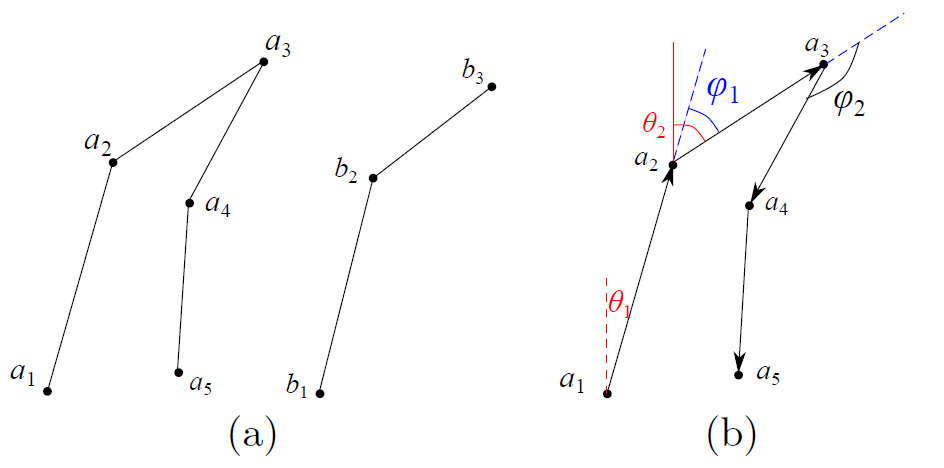
\includegraphics[width=0.8\textwidth]{figure2_1_turnTra}
\caption{轨迹相似计算示例\upcite{liu2012similarity}}
\label{fig:2_3_turn}
\end{figure}
\begin{equation}
\label{equ:chap2:Center_of_mass}
ctr(Tra)=(\bar{x},\bar{y})=(  \frac{\int x f(x)dx  }{\int f(x)dx},\frac{\int y f(y)dy  }{\int f(y)dy} )
\end{equation}
\begin{figure}[htp]
\centering
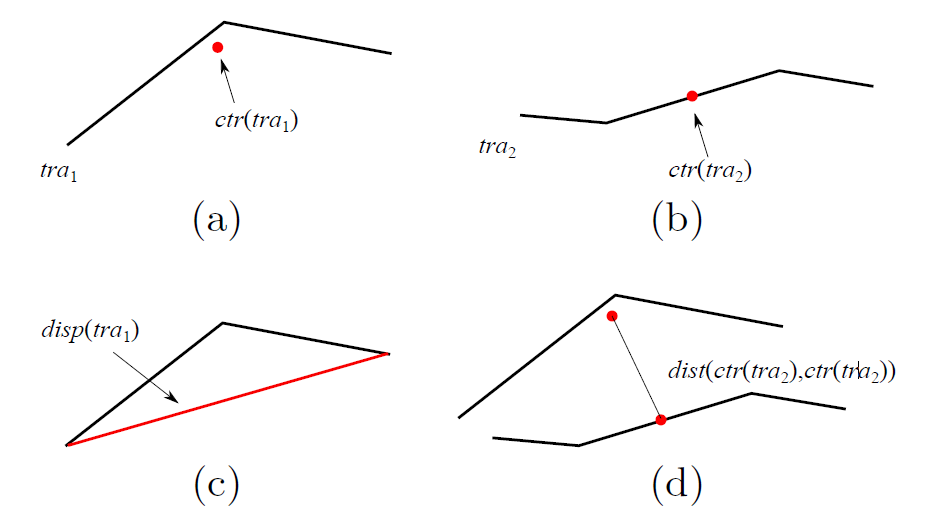
\includegraphics[width=0.8\textwidth]{figure2_1_Center_of_mass}
\caption{基于Center of mass轨迹计算示例\upcite{liu2012similarity}}
\label{fig:2_3_Center_of_mass}
\end{figure}
%-----------------写到这里
\par 采用该算法来计算用户轨迹之间的相似度同直接计算轨迹之间的欧氏距离相比较,能够将轨迹的形状考虑在内,这样能够结合避免直接计算轨迹之间的距离所因为离群点造成了计算结果的巨大偏差。
\subsection{Dynamic Time Warping}
DTW(Dynamic Time Warping)算法最初是由Itakura提出的的一种新型的计算距离的方法\upcite{itakura1987distance},在最初的一段时间是被应用于语音识别领域,在语音识别中即使是同一个词语,由不同的人说出口但是他们的语速、语气等不同造成了单词音频的差别。DTW正由于其计算距离的特殊处理使其能够胜任这一工作。DTW算法采用动态时间规整的思想,将需要比较的两个序列在横轴时间维度上进行压缩、拉伸等操作,使得两条序列具有相同的长度具有更有效的匹配度,同时也消除了传统基于欧式距离计算带来的弊端。
\par 设待计算距离的两个序列,序列$Q$和序列$C$ (两条序列的表示见公式\ref{equ:chap2:dtw_01}、\ref{equ:chap2:dtw_02})。如果两条序列的长度相同,则计算变得很简单。但是如果$m \neq n$,就需要拉伸变形两条序列,使得它们的长度能够尽量对齐同时保留原有序列的信息,算法首先构造一个$n \ast m$矩阵$d$,其中$d[i,j]$ 表示$q_{i}$ 和$c_{j}$之间的距离。采用动态规划的方法来找出序列$Q$和$C$之间的最佳匹配,其中转移方程为找出一条路径使得所有总和的距离$\gamma[i,j]$最小化,具体公式描述见公式\ref{equ:chap2:dtw_03}。
路径及矩阵可视化见图\ref{fig:2_5}。其中:A)为两个待计算比较的序列;B)为通过DTW动态规划求解后两条序列计算距离时所对应的点;C) 将原有序列所对应的位置进行拉伸展开后更加直观的DTW匹配计算结果示意图。
\begin{equation}
\label{equ:chap2:dtw_01}
Q=q_{1},q_{2},…,q_{i},…,q_{n}
\end{equation}
\begin{equation}
\label{equ:chap2:dtw_02}
C=c_{1},c_{2},…,c_{j},…,c_{m}
\end{equation}
\begin{equation}
\label{equ:chap2:dtw_03}
\gamma[i,j]=d[i,j]+min\{\gamma[i-1,j-1],\gamma[i-1,j],\gamma[i,j-1]\}
\end{equation}
\begin{figure}[htb]
  \centering%
  \subfloat[原始序列]{%
    \label{fig:dtw-1}
    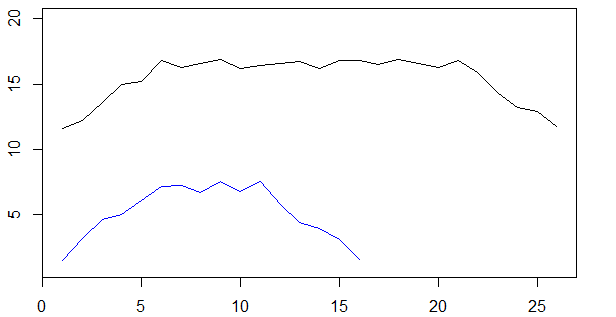
\includegraphics[width=0.4\textwidth]{dtw-1}}\hspace{2em}%
  \subfloat[DTW算法匹配模式结果]{%
    \label{dtw-2}
    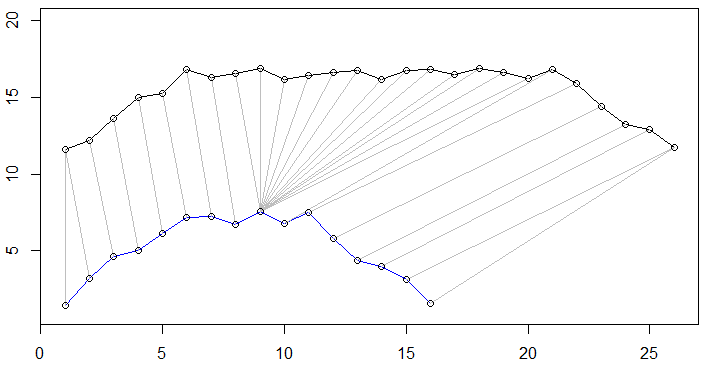
\includegraphics[width=0.4\textwidth]{dtw-2}}\hspace{2em}
    \subfloat[DTW算法拉伸序列计算距离]{%
    \label{dtw-2}
    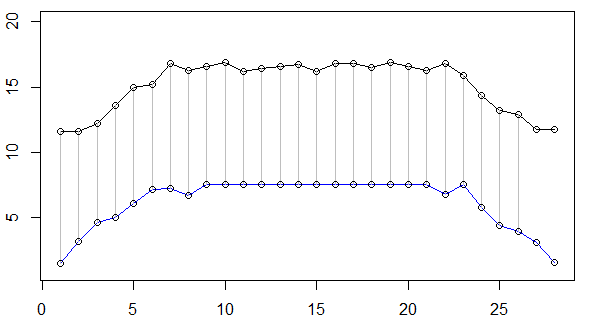
\includegraphics[width=0.4\textwidth]{dtw-3}}
  \caption{DTW算法匹配序列结果示意图}
  \label{fig:2_5}
\end{figure}
\par 通过对DTW算法的原理分析可以得知,序列$Q$和序列$C$的长度越长,则最终计算结果得到的距离就会越大。因此,后者研究中,采用了多种归一化的加权处理方法对结果进行加权处理\cite{ratanamahatana2004everything},获得最优的DTW计算结果。

\section{自然语言处理方法}
\label{sec:section2-3}
相对于用户的空间轨轨迹度量,用户在日常生活中的语义轨迹蕴含了更丰富的上下文信息同时人与人之间在语义轨迹层次上特别是好友之间可能表现出惊人的一致性,如经常去某些地方,在一天中总是先从某个地点出发,再经过某些地点,最后在某个咖啡店相遇等等。基于轨迹的用户模式的交互能够反映出用户在某个空间中的相遇;而基于用户语义轨迹的分析能够在一定程度上展现出用户在社会活动上的相似性,在绪论部分已经详细从社会心理学的研究中描述了人们在现实生活中相遇频率能够反映出用户之间的关系强度,文献\cite{singelis1994measurement}研究发现人们会更加喜欢那些在兴趣、价值观、人格上和自己相似的人。因此通过用户的语义轨迹来在更高的层次上对用户的行为进行相似度计算,进而推测出用户的关系强度。
\par 通过将用户的语义位置序集合同自然语言处理中的文档进行对比, 可以借鉴自然语言处理的算法来处理用户的语义轨迹序列。用户每天的活动轨迹通过语义标签标注后,得到的是一个现实生活中语义轨迹的序列集合,如将一个用户的活动轨迹表示为$<寝室,食堂,教室,图书馆,...,公园>$,通过结合自然语言文档文档相似性计算的思路,把用户每天所计算得到的语义轨迹作为一条原始自然语句,用户在$n$天内所采集的所有轨迹记录就生成了一篇文档,最后基于自然语言处理方法通过计算用户语义轨迹生成的文档之间的相似性来表示用户之间的关系强度。
\par 在以往的研究中,通常使用编辑距离来衡量语句的相似性。在用户轨迹相似分析上,文献\cite{farrahi2008did}借助了LDA主题模型来计算用户语义轨迹之间的相似性,后来的研究在其其基础上对计算方法进行了改进\upcite{yangruosong}。其算法改进在于基于LDA主题模型,将用户的所有语义轨迹看作一篇文档来训练出若干个主题。在计算用户轨迹相似性的时候,将用户用户估计输入到训练好的LDA模型中,然后采用余弦相似度分析比较二者输出的主题分布集合之间的相似度,作为这两个用户之间的关系强度。
\par word2vec是Google在2013年开源的一种词向量计算算法\upcite{mikolov2013efficient}, word2vec借鉴深度学习方法,将文本通过训练的得到文本的$K$维向量表示,通过词与词之间的距离来计算它们之间的相似度。
\subsection{LDA主题模型}
2003年文献\cite{blei2003latent}提出了LDA(Latent Dirichlet Allocation)模型对自然语言进行建模,可以用来识别文档语料中潜在的主题信息。整个计算模型采用了词袋的计算方法,计算出文档的向量表示,每一篇文档计算出一部分主题的概率分布,而每一个主题内又可以表示为很多词语的一个概率分布,LDA的训练过程为:遍历每一个文档,在主题分布袋中随机抽取一个主题;然后在被随机抽取到的主题中再随机抽取一个单词;最后重复上述步骤直到遍历完文档中的所有词语。整个生成的过程可以用图\ref{fig:2_6}表示:对于每一份文档与设定的$T$个主题之间的概率分布对应$\theta $,每个主题与词袋中的$V$个词语之间的概率分布$\phi$,其中$\theta $和$\phi$分别有一个参数$\alpha$和$\beta$的狄利克雷的先验分布,这样对于任意一份文档$d$中的每一词语,我们从与文档相对应的概率分布$\theta $中选取一个主题$z$,随即在根据与主题$z$对应的概率分布$\phi$中选取一个词语$w$,最后重复上述过程$N_{d}$次,就能够产生文档$d$,公式\ref{equ:chap2:lda_01}为LDA的核心公式。
\begin{figure}[htp]
\centering
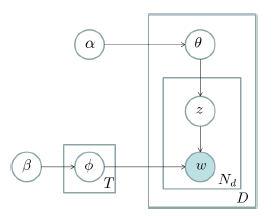
\includegraphics[width=0.6\textwidth]{figure2_6_lda}
\caption{LDA的图模型表示}
\label{fig:2_6}
\end{figure}
\begin{equation}
\label{equ:chap2:lda_01}
p(w|d)=p(w|t) \ast p(t|d)
\end{equation}
% 写到了这里------------------
\subsection{word2vec}
word2vec是Google在2013年开源的一种词向量计算算法\upcite{mikolov2013efficient}, word2vec借鉴深度学习方法,将文本通过训练的得到文本的$K$维向量表示,也就是说把特征转换到了$K$维空间进行表示,通过词与词之间的距离来计算它们之间的相似度。word2vec采用了三层的神经网络结构即为输入层-隐含层-输出层构成,其主要方法是借助哈夫曼编码针对相似词频的词语构建出相似的隐藏层激活函数,算法采用了层次化的Log-Bilinear模型,其中一种是基于CBOW(Continuous Bag-of-Words Model)的计算模型,在CBOW模型中,根据上下文信息可以预测下一个词语$w_{t}$,其公式如\ref{equ:chap2:word2vec_01}所示,CBOW的计算模型如图\ref{fig:2_7_cdow}所示。
\begin{equation}
\label{equ:chap2:word2vec_01}
p(w_{t}|context)=p(w_{t}|w_{t-k},w_{t-k+1},\cdots ,w_{t-1},w_{t+1},\cdots w_{t+k})
\end{equation}
\par 现在的CBOW计算采用层次的Softmax算法,每个单词$w_{i}$都可以有一条从根节点出发被唯一访问到的路径,这条路径就形成了词语的编码。
\begin{figure}[htp]
\centering
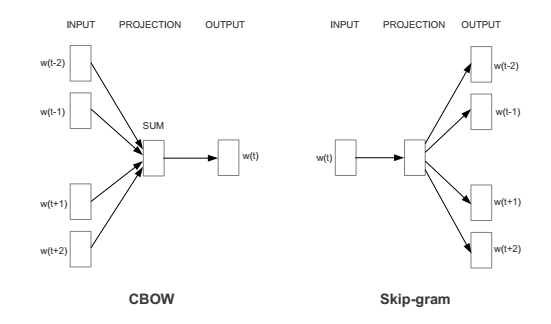
\includegraphics[width=0.8\textwidth]{figure2_7_cdow}
\caption{word2vec神经网络结构图\upcite{mikolov2013efficient}}
\label{fig:2_7_cdow}
\end{figure}
\begin{figure}[htp]
\centering
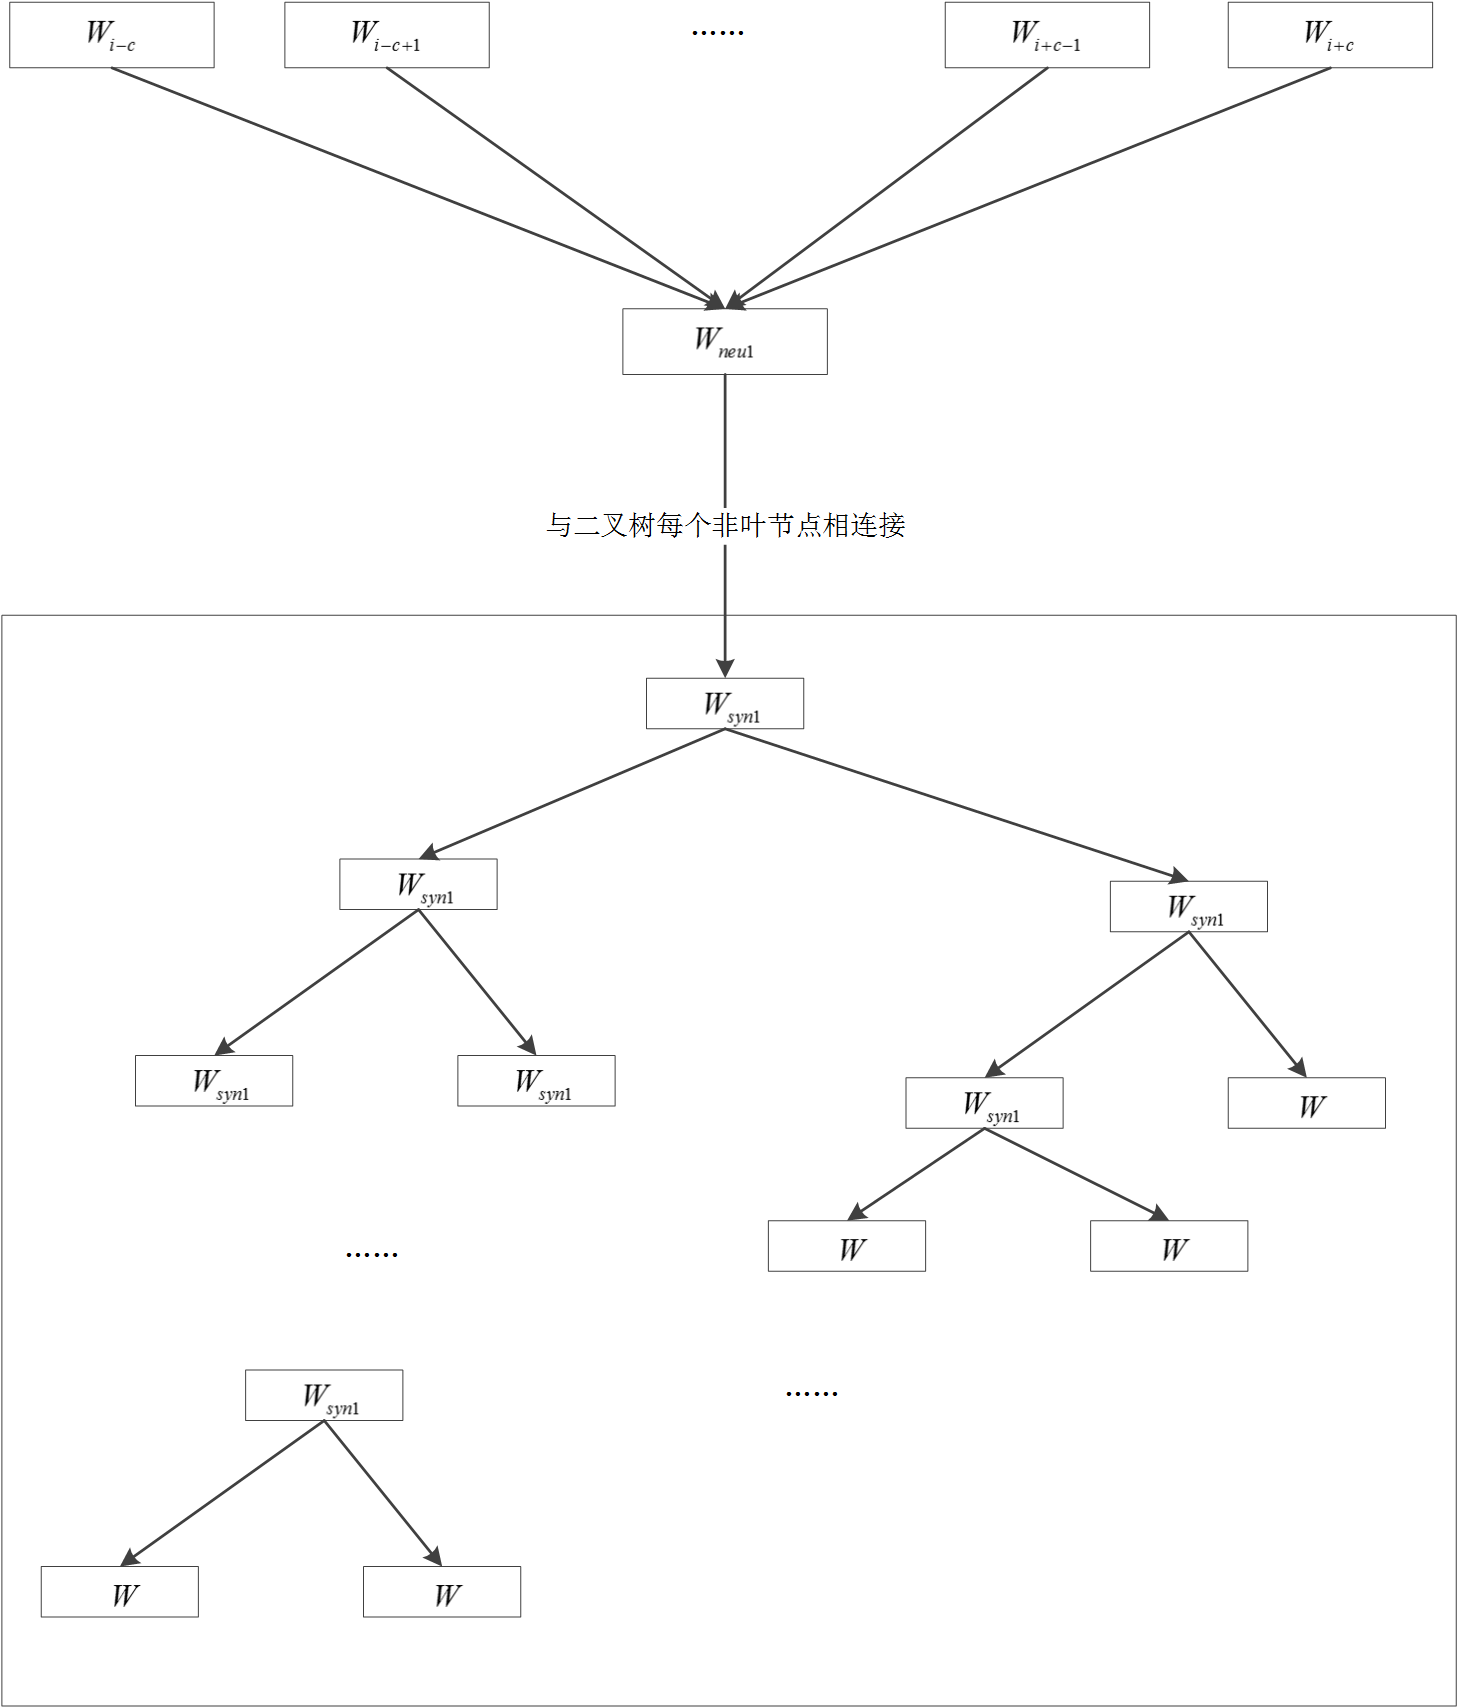
\includegraphics[width=0.7\textwidth]{figure2_7_w2cmodel}
\caption{word2vec神经网络结构图}
\label{fig:2_7}
\end{figure}
\par 在图\ref{fig:2_7}中,第一层也称之为输入层, 它的输入是词向量;中间的层次为隐含层,得到的的输入是输入层若干个词向量的向量累加结果;第三层则是由二叉树所构成的霍夫曼树所组成的输出层,其中每个非叶节点是一个计算后的向量但是不同于输入层的词向量,这里计算后的向量不代表某个词语,而是表示一个类别的词语,同时这棵霍夫曼树的所有叶子节点包含了输入词袋中的所有词。
\par 对于词袋$BG$中的单词$w$,在图\ref{fig:2_7}中一定能够找到有且仅有一条从Root节点到叶子节点$w$的路径。路径中的每一次分支都是一个概率问题,因此得到\ref{equ:chap2:word2vec_01}中的数学表达式,将其中的$w_{i}$用词向量替换,得到该三层神经网络的目标公式如\ref{equ:chap2:w2v_03}, $Num^{w}$表示从Root节点到词向量节点$w$路径中包含的节点个数,$w_{j}$表示该路径上的第$j$个词,$v_{w}$表示词$w$对应的词向量,$\sigma$表示SIGMOID函数,通过求解目标函数的最大值,就可以得到每个词所对应的向量。
\begin{equation}
\label{equ:chap2:w2v_03}
L=\sum_{w\in C}\sum_{j=2}^{Num^{w}}\{(1-w_{j})log[\sigma(v_{w}^{T}\theta_{j-1}^{w})]+w_{j}log[1-\sigma(v_{w}^{T}\theta_{j-1}^{w})]\}
\end{equation}
\subsection{快速Hash算法}
基于word2vec的计算方法针对文档的分词结果,再根据神经网络模型计算得到每个词的向量表示,但是这样无疑增加了整个计算过程的时间复杂度,本文研究目的是能够为众多用户提供一种计算关系强度的框架,因此如果采用传统的Hash算法进行处理,则能够减少程序的运行时间,来自于GoogleMoses Charikar针对海量文档快速计算相似计算提出了一种局部敏感hash算法\upcite{manku2007detecting},其核心内容恰巧和word2vec相反:希望将数据进行降维处理,将原始的高维词向量通过一系列运算映射到低维的词向量,最后来计算相似性。
\par 以上介绍了几种方法在自然语言处理中都得到了广泛的应用,因此综合考虑使用最后一种方法来作为计算方法, 在后面还会详细讲解如何使用hash来度量用户之间的关系强度,以及在不同处理方法之间进行横向和纵向的比较。
\section{WiFi和蓝牙数据的度量方法}
WiFi和蓝牙作为一种主动对外界感知和探索所得到的感知信息,已经证实能够被用来分析用户之间的社交关系。文献\cite{hsu2007mining}通过收集到用户的WiFi数据,然后将用户的WiFi数据同现实语义位置进行关联,得到了WiFi的语义向量,这样就能够得到基于WiFi的用户活动轨迹序列,提出了一种新的模型AMVD(average minimum vector distance)来计算人与人之间的距离,其计算公式如\ref{equ:chap2:amvd}所示,其中$a_{i}$和$b_{j}$表示用户A和用户B之间的联合向量,$d(a_{i},b_{j})$表示计算二者向量之间的曼哈顿距离。
\begin{equation}
\label{equ:chap2:amvd}
AMVD(A,B)=\frac{1}{\left | A \right |}\sum_{\forall a_{i} \in A}^{ }  \mathop{\arg\min}_{\forall b_{j} \in B} d(a_{i},b_{j})
\end{equation}
\par 蓝牙数据和GPS轨迹数据都能够推测出用户之间的交互行为,蓝牙作为一种近距离的无线通讯手段,收到波长影响使得通讯距离只能是5-10米内,因此蓝牙感知数据能够进一步描述了用户之间在现实生活中的物理接触。前人的研究中,有根据蓝牙信息来简单计算出用户在现实空间中的面对面交互次数,从而推测出用户的社会关系情况\upcite{eagle2009inferring,zheng2013unsupervised}。在本文中,我们使用了新的数据结构来表示用户的WiFi、蓝牙感知数据,同时直接计算其感知上下文环境信息的相似度作为用户之间环境的相似度的参照。
\section{小结}
\label{sec:section2-4}
本章详细的从本课题研究的三个数据源出发对不同数据源的研究方法、现状进行了详细的分析和讨论。2.1节讨论了在用户原始GPS轨迹数据处理中要解决的三个主要问题:剔除异常点、停留点检测以及空间轨迹的聚类。2.2节则是介绍了计算用户轨迹序列相似度的常用方法,并以此结果作为用户的关系强度计算结果。2.3节从自然语言处理的角度介绍了常用的文档相似性检测计算方法,为计算用户语义轨迹的相似度提供了可行性算法。2.4节从WiFi和蓝牙数据处理计算角度出发,介绍了前人研究的计算方法理论,为本研究中所采取的基于上下文环境的计算方式作出铺垫。
\chapter{RSMHD用户关系强度计算框架模型}
\label{chap:chapter07}
上一章详细介绍了和本研究数据源相关的处理技术与方法,接下来这一章将主要介绍RSMHD的多维据源多维度的关系度量模型的整体框架结构。
\section{RSMHD模型框架描述}
\label{sec:section7-1}
本研究的主要内容是通过采集到的用户感知数据(GPS轨迹信息 、WiFi数据、蓝牙数据)来开展用户之间的关系强度度量工作。因此本文希望能够提供一种基于此类非社交的感知数据建立的通用的用户关系强度计算框架。非社交数据主要是指不是来自于用户直接社交活动中所收集到的数据,在本研究中主要包含了用户轨迹数据、用户WiFi感知数据和用户蓝牙感知数据。因此本课题基于以上三种不同的感知数据源提出了能够统一处理多种数据源的计算框架,其整体概要结构图如图\ref{fig:7_1}所示,图中描述整体架构由以下几部分组成:上下文感知收集模块、基于用户日常轨迹的关系强度计算模块、基于用户WiFi感知数据的关系强度计算模块和基于用户蓝牙的关系强度计算模块。用户的日常语义轨迹是有连续的GPS位置点所组成的轨迹的集合,在用户的轨迹信息的采集过程中,因受到地形、气候、GPS 传感器的干扰误差的影响,会出现GPS漂移现象,GPS的位置漂移使得用户的轨迹数据中存在大量的噪音数据,影响后续对数据的处理和分析。因此对采集到的用户轨迹数据采取滤波处理,消除轨迹中所蕴含的噪音数据。GPS 位置的采集还受到地形环境的影响,在室内无法获取GPS 位置信息的时候会导致用户轨迹的缺失,造成计算结果产生巨大偏差。第四章部分将重点针对上述问题展开GPS轨迹的处理研究工作,以获得好的信息效果。对于剩余的WiFi和蓝牙感知数据来讲,主要的工作是针对二者数据源的特点以及后续的算法输入对原始数据进行提取和结构化建模表示存储。第四章的其余部分将会针对WiFi和蓝牙感知数据的预处理和结构化表示进行详细的描述。
\begin{figure}[htp]
\centering
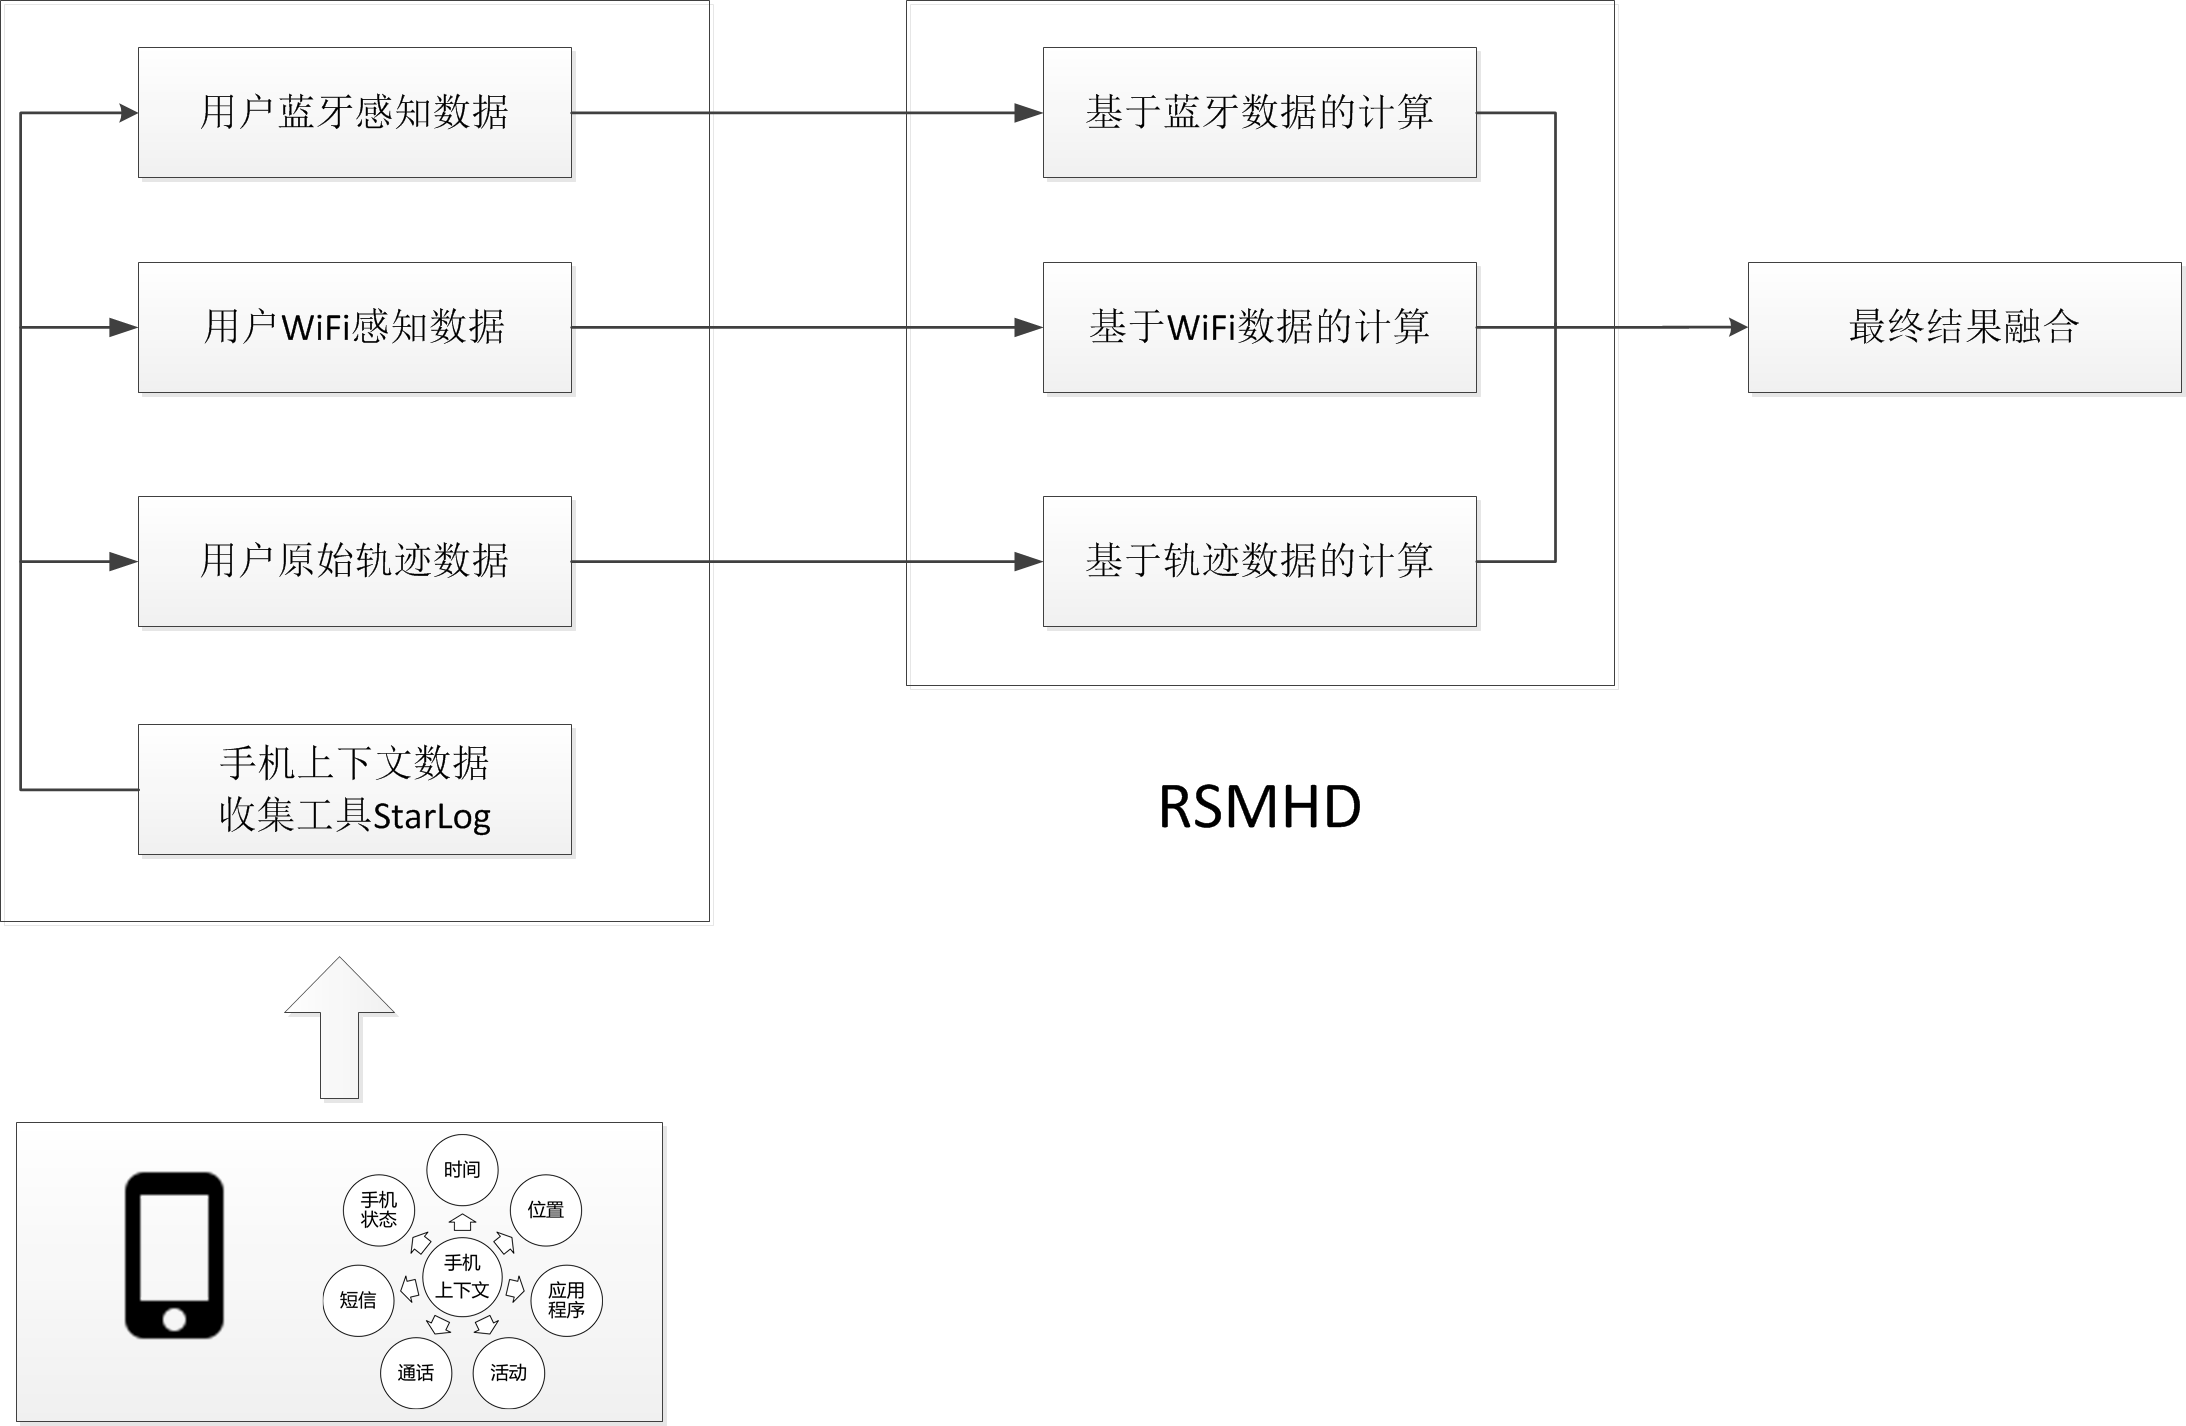
\includegraphics[width=0.8\textwidth]{figure7_1_RSMHD}
\caption{RSMHD用户关系强度计算模型框架图}
\label{fig:7_1}
\end{figure}
\subsection{基于轨迹数据的关系强度计算模块概述}
在本研究中所提出的RSMHD计算框架模型中,第二层需要基于用户的日常语义轨迹分别通过计算地理轨迹相似性、用户的语义轨迹相似性以及日常轨迹运动模式三个层次关系强度融合为轨迹强度结算结果,其详细框架图如图\ref{fig:7_1_tra}所示。在这个模块中,通过计算用户日常地理轨迹的相似性推测出用户之间的关系强度;针对用户活动产生的日常语义轨迹,RSMHD 模型采利用自然语言处理的思想,通过快速编码变换计算出用户基于语义轨迹的关系强度;第三层中,RSMHD 进一步挖掘出用户轨迹中更高一层的上下文信息(High Context)得出用户日常轨迹模式如:用户A 经常喜欢到校外某地用餐、用户B 经常下午在操场跑步等这些代表用户日常轨迹活动模式的信息,计算用户之间基于运动模式的关系强度。
\begin{figure}[htp]
\centering
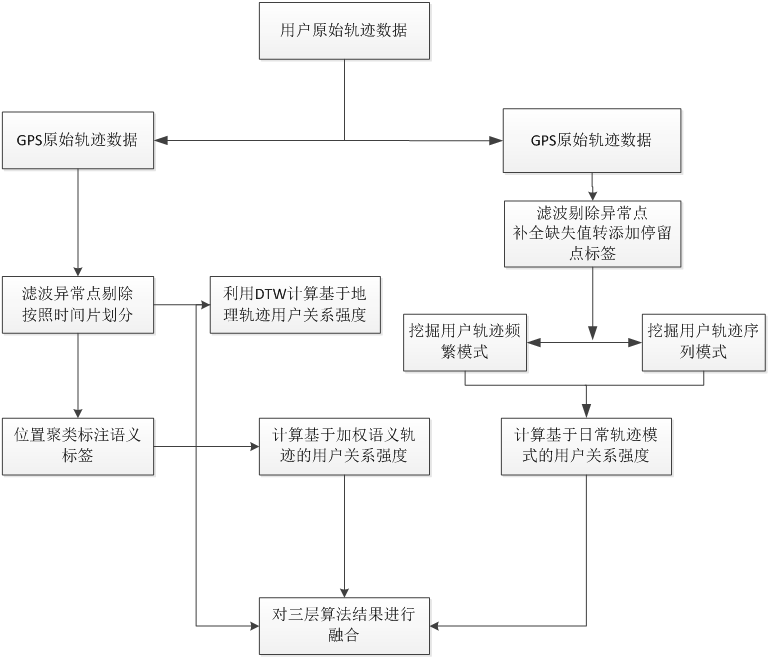
\includegraphics[width=0.8\textwidth]{figure7_1_tra}
\caption{RSMHD中基于用户轨迹计算模块详细框架图}
\label{fig:7_1_tra}
\end{figure}
\subsection{基于WiFi和蓝牙数据的关系强度计算模块概述}
在RSMHD计算框架模型中我们针对WiFi和蓝牙原始数据的特点以及现实生活中WiFi和蓝牙上下文环境的特征,采用了区别于原有基于WiFi和蓝牙计算社交关系的方法,整体的详细计算框架如图\ref{fig:7_1_wifi}所示。在WiFi和蓝牙数据处理计算框架中,分别针对底层手机的上下文感知信息进行数据信息的提取的规整,从复杂冗余的信息中萃取出关键的富有价值的信息;然后结合WiFi和蓝牙各自的上下文环境特征信息,将整理后的数据用图的数据结构进行结构化表示,使得抽象表示后的数据结构更加符合现实中的含义;最后基于结构化后的感知数据进行关系强度计算,将结果输出到下一层。
\begin{figure}[htp]
\centering
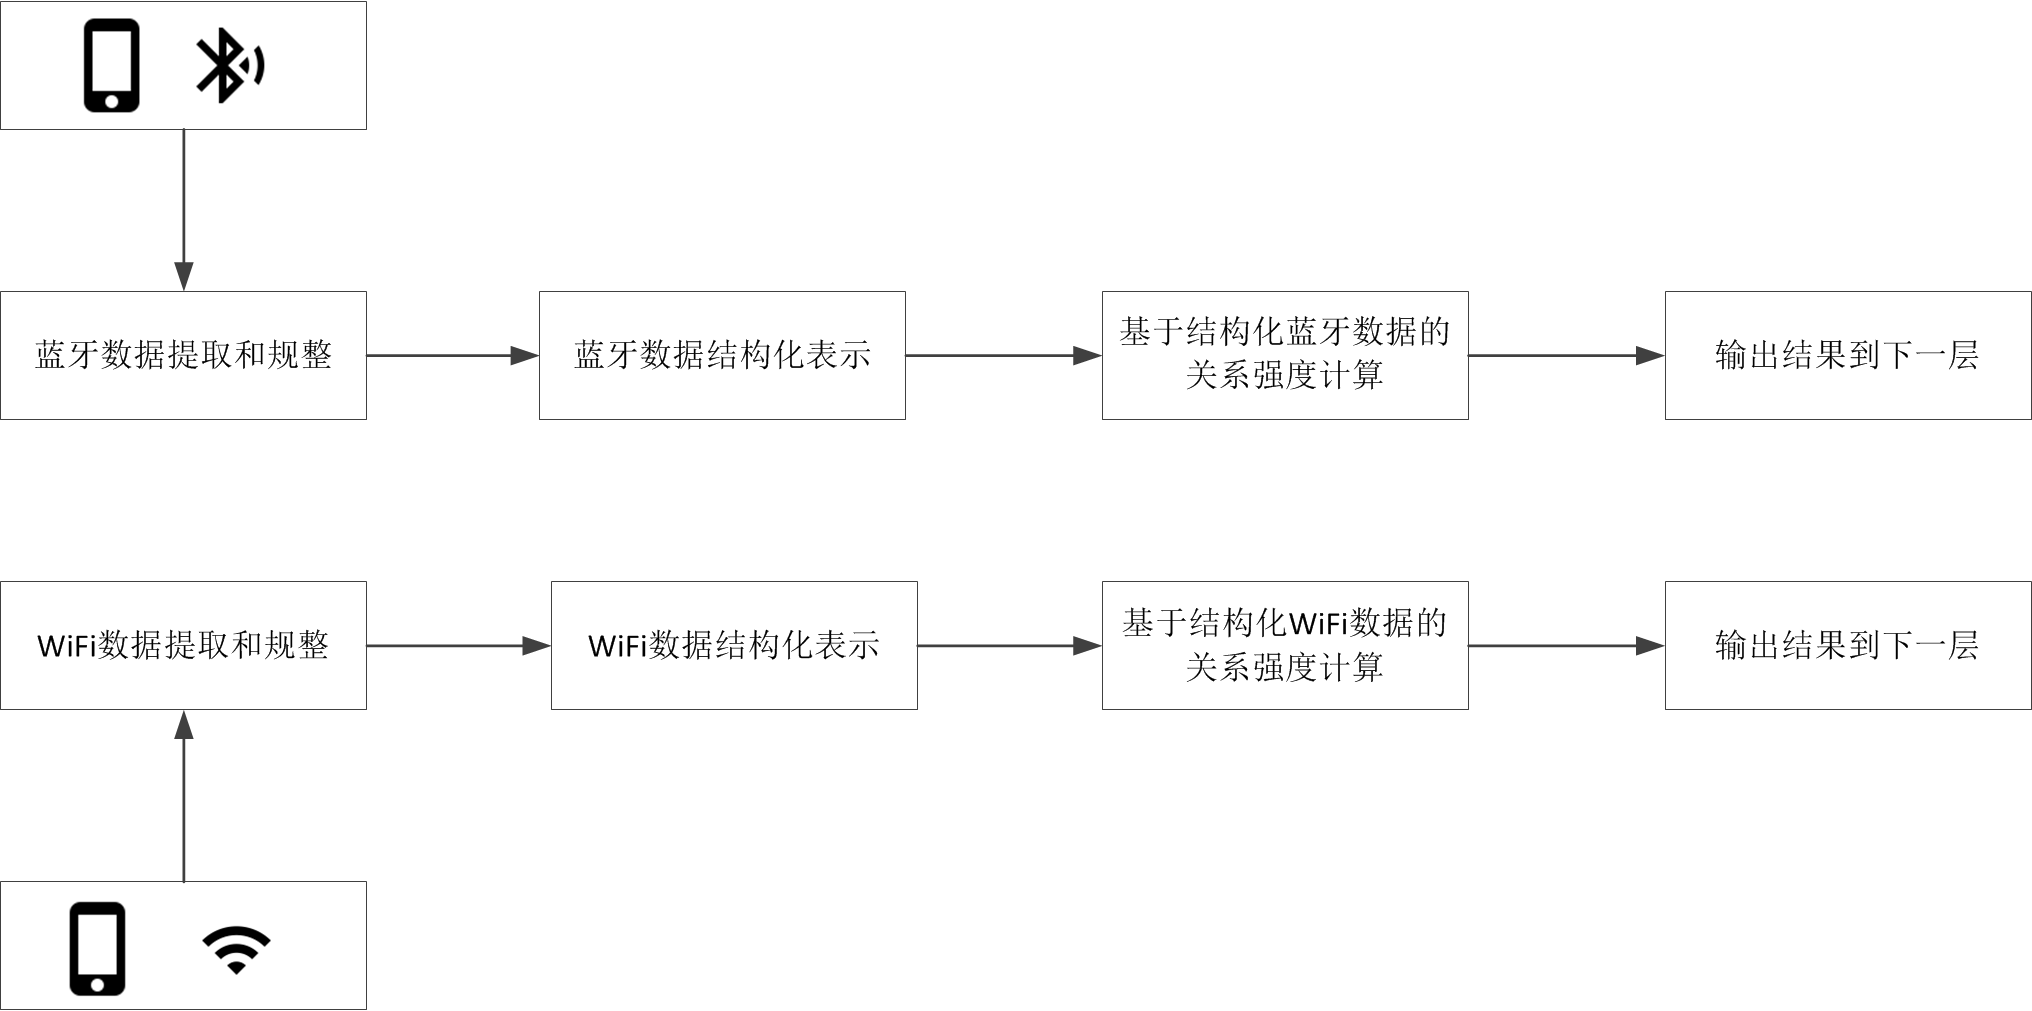
\includegraphics[width=0.8\textwidth]{figure_3_RSMHDwifibluee}
\caption{RSMHD中基于WiFi和蓝牙计算模块详细框架图}
\label{fig:7_1_wifi}
\end{figure}
\section{RSMHD模型计算流程概述}
\label{sec:section7-2}
整个信息采集是采用我们自己编写的用户手机上下文信息收集工具StarLog来记录保存用户手机的上下文感知数据如:GPS位置信息、WiFi感知信息、蓝牙感知信息、脱敏的通话记录、短信记录、APP使用记录等。
\par 针对用户的GPS位置数据我们首先对轨迹数据进行预处理,即采用滤波算法检测出用户日常轨迹中的漂移点减少轨迹中的噪音;然后根据停留点检测算法识别出用户轨迹中的停留点,针对缺失的轨迹点进行预测补全;第一层次中针对用户日常空间轨迹相似性计算时,可用将每天的轨迹数据划分为若干时间片的数据,然后采用DTW加权算法对时间片内的空间轨迹相似度进行计算并按照一天的轨迹进行处理。对于基于用户语义轨迹推倒关系强度这层我们首先将得到的停留点进行聚类分析,得到聚类后的停留点集合因此对于每一个簇都是同一个语义位置,然后将聚类GPS转换为现实社会中的语义标签,在计算用户语义轨迹的相似性时,采用快速hash算法将用户分片后的语义轨迹序列作为输入,得到用户之间每天的语义轨迹相似度,以及最终的语义轨迹相似度并将结果作为用户自己的关系强度。在上一层的基础上,我们针对得到的用户语义估计进行挖掘,寻找出用户的日常运动模式,然后计算用户运动模式之间的相似度并作为关系强度之一进行输出,综合三层的计算结果得到用户基于轨迹数据计算得到的关系强度。
\par 其次针对用户的WiFi和蓝牙数据,首先从原始数据中提取出重要的信息,并将WiFi和蓝牙数据进行结构化存储处理,采用图的存储结构,将WiFi和蓝牙数据还原为现实生活中的存在环境,然后针对用户切片时间内每刻的感知环境进行相似度计算,并将一天中的计算结果进行汇总进一步得到所有时间段内的用户相似度,最后将结果作为基于两种数据源推测出的用户关系强度。
\par 最后,在基于前面三种数据源的用户关系强度计算结果的基础上,采用集成学习的思想对计算结果进行融合处理,得到最终的用户关系强度计算结果。

\chapter{RSMHD框架的相关技术研究}
\label{chap:chapter03}
上一章节主要是对本课题研究的RSMHD框架进行了详细的描述,本章接下来将针对每一个模块中的具体面对的问题以及采取的方法进行详细描述,包括噪音点的剔除、如何语义轨迹、如何计算轨迹相似性以及如何对WiFi和蓝牙数据进行结构化处理等。
\section{GPS轨迹处理计算技术}
\label{sec:section3-1}
用户的日常GPS轨迹数据包含了用户的生活工作以及娱乐等丰富的上下文信息,如图\ref{fig:tramodel}所示,我们基于用户的日常轨迹分别从地理位置相似性、语义轨迹相似性以及轨迹模式相似性出发度量人与人之间的关系强度。模块的输入是由StarLog收集的GPS感知数据,通过对初始数据的解析提取得到原始的GPS位置点构成的用户轨迹序列。预处理阶段主要是通过滤波算法对原始轨迹序列进行异常点检测,并通过轨迹预测补全缺失的部分GPS轨迹序列;第二层中将第一层得到的停留点赋予语义得到用户的语义轨迹序列,采用自然语义处理思想计算基于语义轨迹的相似性;再往上一层,从用户的历史轨迹数据中挖掘出的频繁模式和序列模式能够反映出用户的日常轨迹运动习惯和行为规律,运动模式在现实生活中表现为用户经常行走的路径序列,是用户轨迹数据规律的抽象表示,最后计算用户之间的关系强度。
\begin{figure}[htp]
\centering
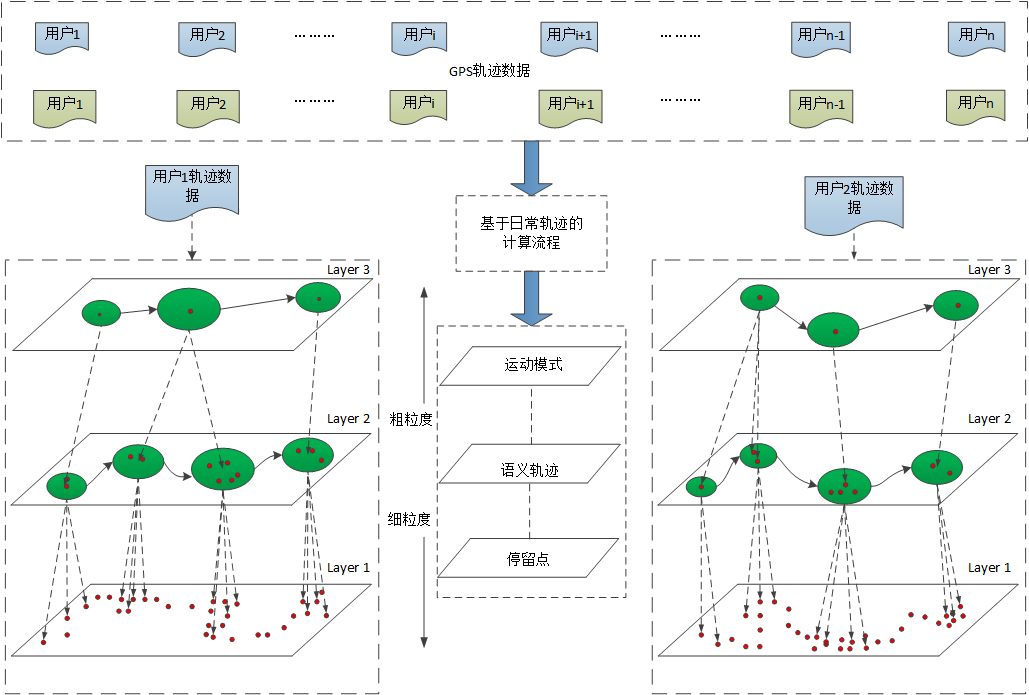
\includegraphics[width=0.8\textwidth]{figure4_2}
\caption{基于多层次多粒度轨迹的用户关系强度计算}
\label{fig:tramodel}
\end{figure}
\section{GPS轨迹预处理与语义化}
\label{sec:section3-2}
本节主要讲述如何对GPS轨迹数据进行清洗规整,以及得到用户的语义轨迹进行结构化存储。
\subsection{剔除轨迹中的异常点}
前文已经提到,由于在获取GPS位置信息的时候会受到位置漂移的影响,导致在获取用户实际位置的时候可能产生采样的误差甚至跳跃,为了使得最终计算得到的关系强度结果更为准确我们需要对GPS轨迹数据进行滤波分析。在第二章中描述了常用的三种滤波方法,在本章中将会针对三种滤波算法进行最后结果展示并根据结果分析最终采用此滤波算法的原因。
\par 首先接下来使用我们自己开发的用户感知数据收集软件StarLog,来分析观察各种滤波算法对用户轨迹中异常点检测剔除的效果,如图如图\ref{fig:3_2_1}、\ref{fig:3_2_2}所示。
\begin{figure}[htb]
  \centering%
  \subfloat[原始轨迹数据]{%
    \label{fig:3_2_1_1}
    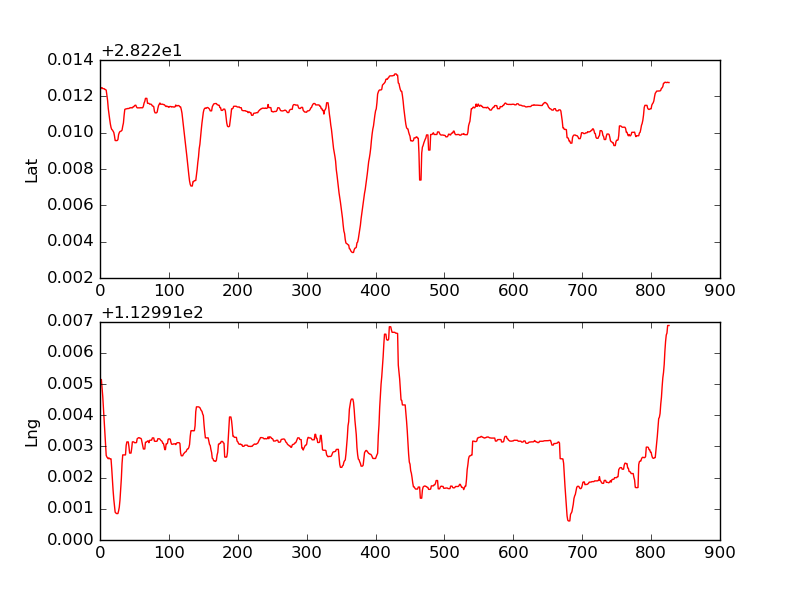
\includegraphics[height=4cm]{figure_4_mid_location1}}\hspace{4em}%
  \subfloat[中值滤波后的轨迹数据]{%
    \label{fig:3_2_2_1}
    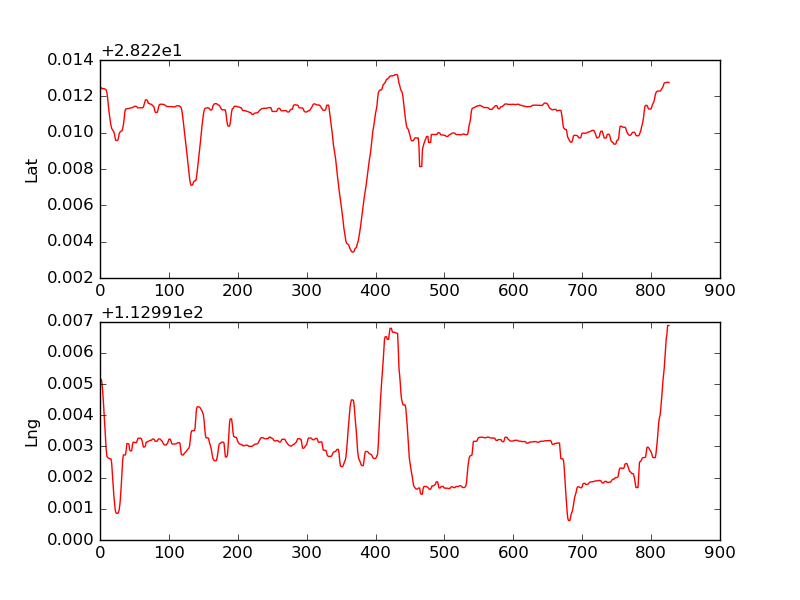
\includegraphics[height=4cm]{figure_4_mid_location1_ed}}
  \caption{轨迹中值滤波实验结果1}
  \label{fig:3_2_1}
\end{figure}
\begin{figure}[htb]
  \centering%
  \subfloat[原始轨迹数据]{%
    \label{fig:3_2_2_1}
    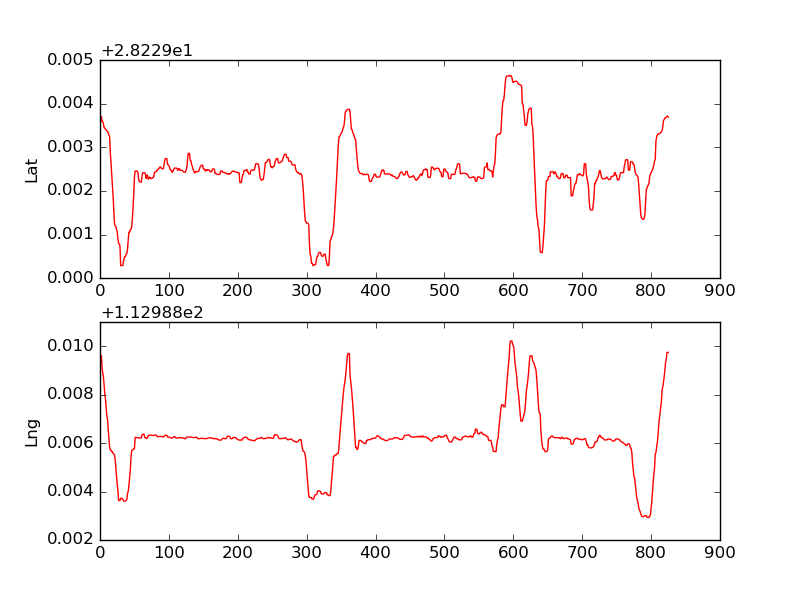
\includegraphics[height=4cm]{figure_4_mid_location2}}\hspace{4em}%
  \subfloat[中值滤波后的轨迹数据]{%
    \label{fig:3_2_2_2}
    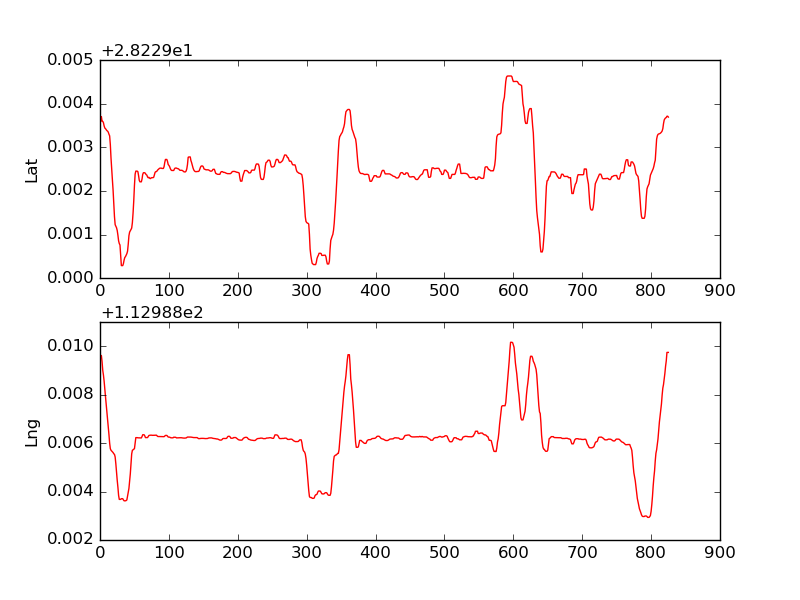
\includegraphics[height=4cm]{figure_4_mid_location2_ed}}
  \caption{轨迹中值滤波实验结果2}
  \label{fig:3_2_2}
\end{figure}
\par 从实验结果中我们可以观察到虽然中值滤波能够过滤掉其中少部分的位置漂移点,但是针对于一些明显的轨漂移点却没有能够很有效的识别过滤。
\par 接下来我们再使用均值滤波算法对用户轨迹进行分析,观察均值滤波算法对用户轨迹中异常点的检测情况,部分实验结果见图图\ref{fig:3_3_1}、\ref{fig:3_3_2}。
\begin{figure}[htb]
  \centering%
  \subfloat[原始轨迹数据]{%
    \label{fig:3_2_1_1}
    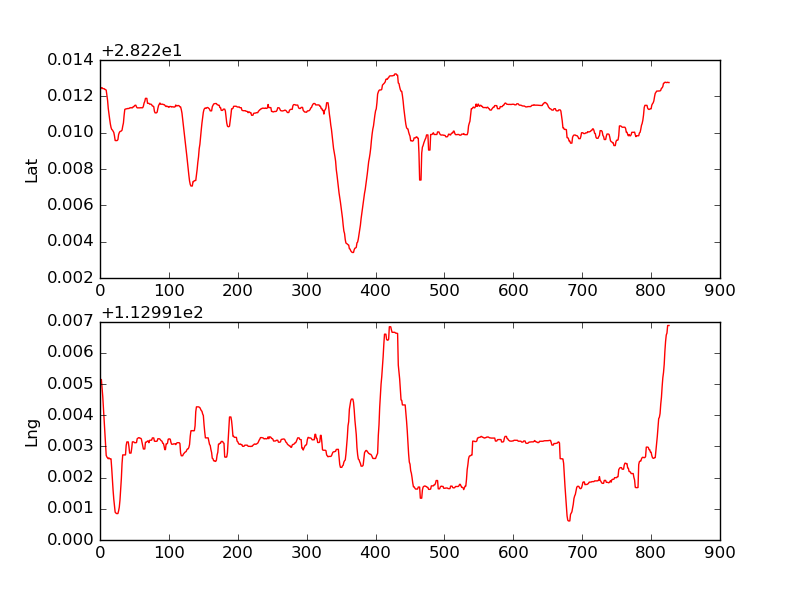
\includegraphics[height=4cm]{figure_4_mid_location1}}\hspace{4em}%
  \subfloat[均值滤波后的轨迹数据]{%
    \label{fig:3_2_2_1}
    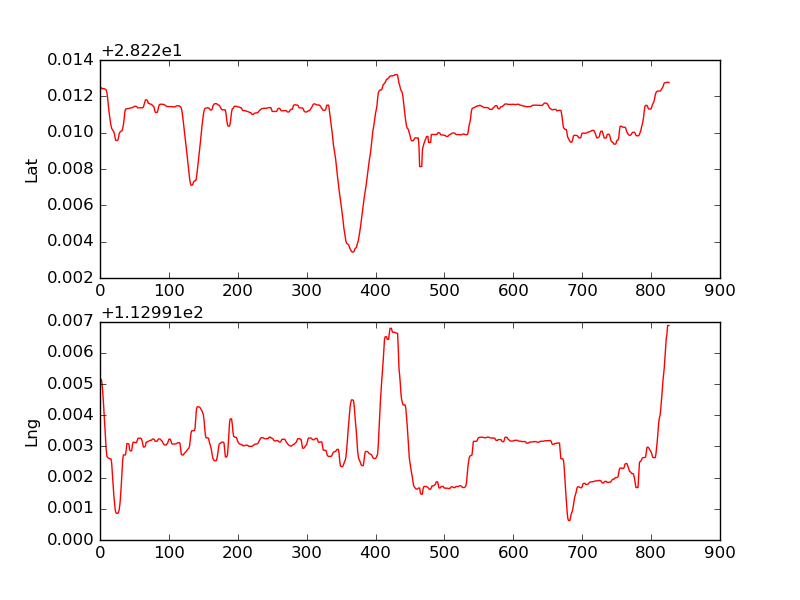
\includegraphics[height=4cm]{figure_4_mid_location1_avg}}
  \caption{轨迹均值滤波实验结果1}
  \label{fig:3_3_1}
\end{figure}
\begin{figure}[htb]
  \centering%
  \subfloat[原始轨迹数据]{%
    \label{fig:3_2_2_1}
    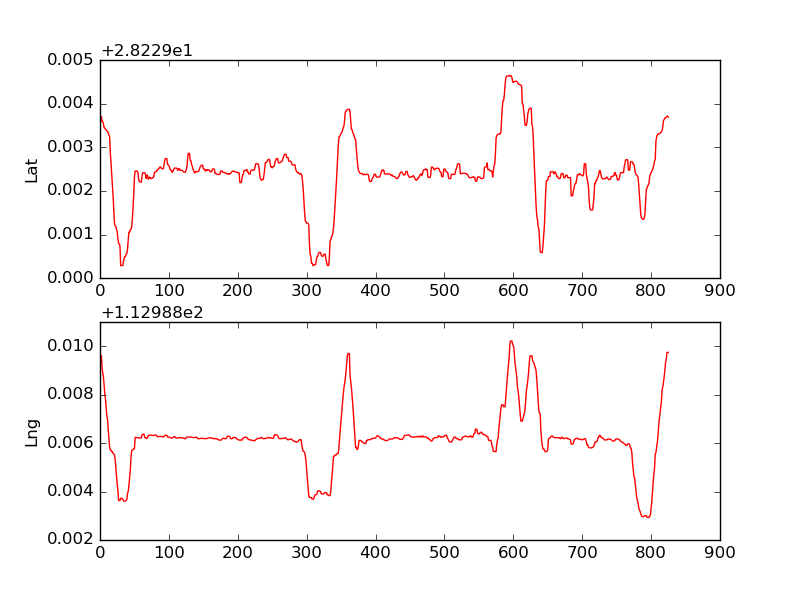
\includegraphics[height=4cm]{figure_4_mid_location2}}\hspace{4em}%
  \subfloat[均值滤波后的轨迹数据]{%
    \label{fig:3_2_2_2}
    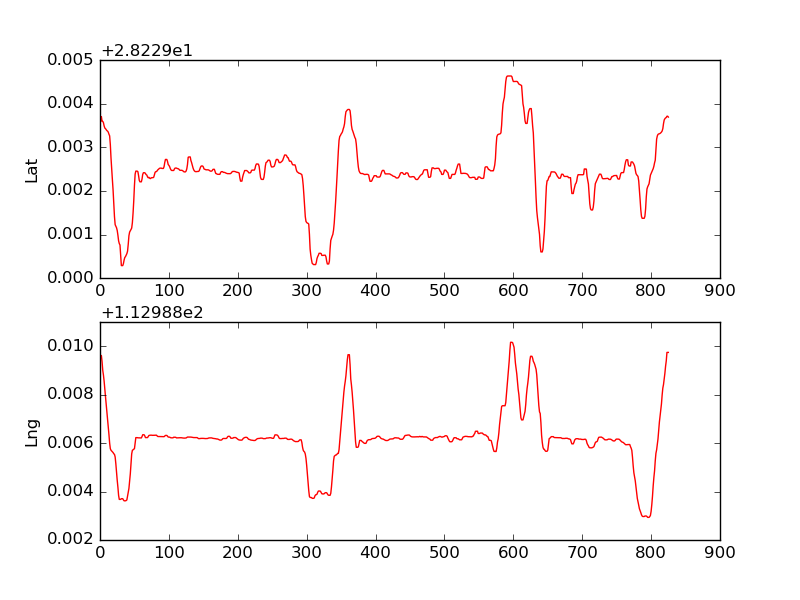
\includegraphics[height=4cm]{figure_4_mid_location2_avg}}
  \caption{轨迹均值滤波实验结果2}
  \label{fig:3_3_2}
\end{figure}
\par 通过对比观察滤波结果图可以发现,相对于中值滤波,均值滤波能够较好的平滑用户的轨迹变化曲线,剔除GPS漂移点。但是,同样无法很有效的处理漂移偏差大的位置点。
\par 通过采取卡尔曼滤波算法得到的用户轨迹如图\ref{fig:3_4_1}、\ref{fig:3_4_2},根据观察图中滤波后的用户轨迹数据,我们可以发现虽然图形变得平滑了许多,但是却使得原有的轨迹信息收到了模糊,难以有效的将两个用户轨迹进行相似度计算。
\begin{figure}[htb]
  \centering%
  \subfloat[原始轨迹数据]{%
    \label{fig:3_2_1_1}
    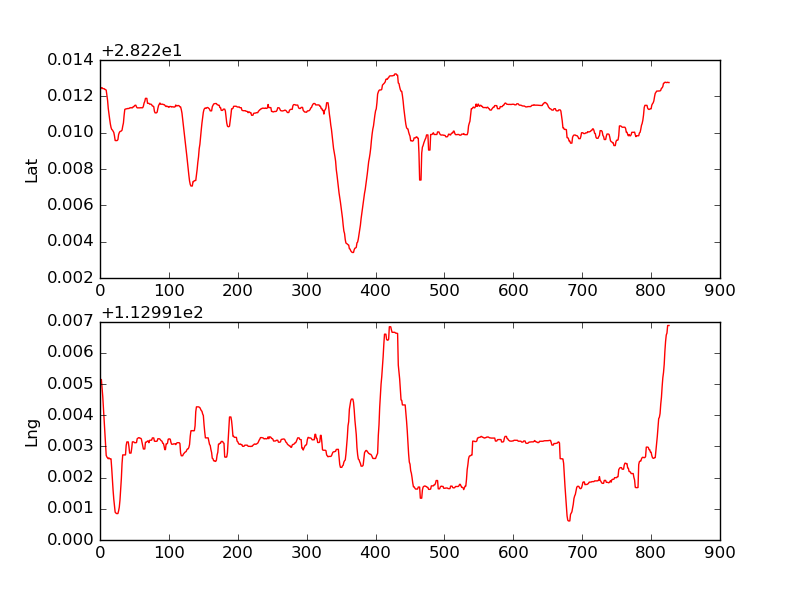
\includegraphics[height=4cm]{figure_4_mid_location1}}\hspace{4em}%
  \subfloat[卡尔曼滤波后的轨迹数据]{%
    \label{fig:3_2_2_1}
    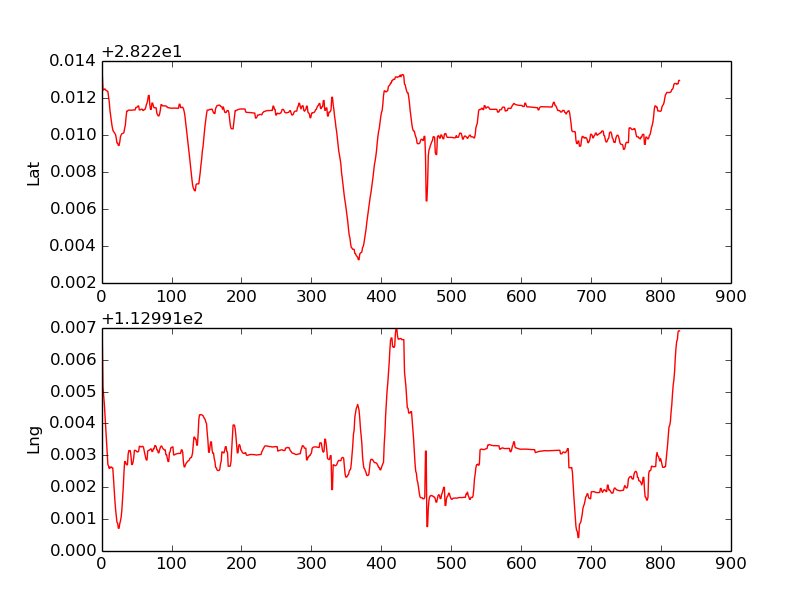
\includegraphics[height=4cm]{figure_4_mid_location1_kalman_ed}}
  \caption{卡尔曼滤波实验结果1}
  \label{fig:3_4_1}
\end{figure}
\begin{figure}[htb]
  \centering%
  \subfloat[原始轨迹数据]{%
    \label{fig:3_2_2_1}
    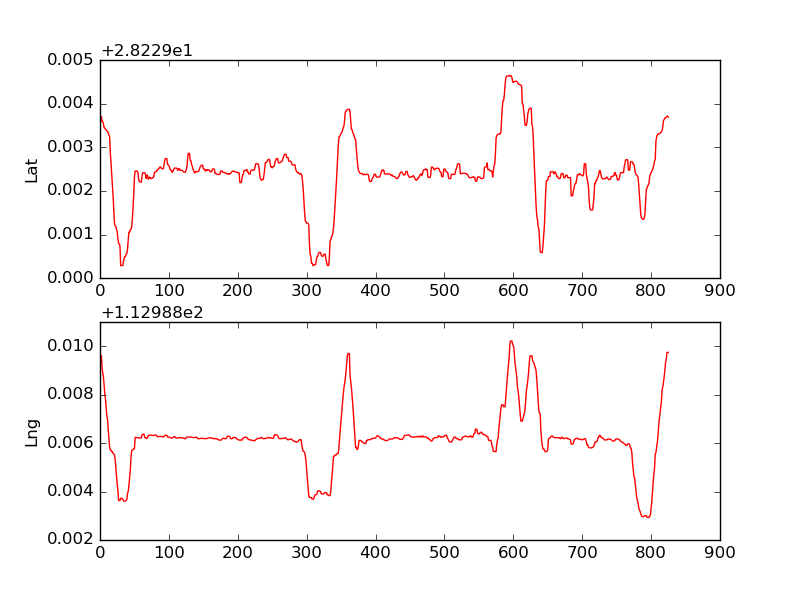
\includegraphics[height=4cm]{figure_4_mid_location2}}\hspace{4em}%
  \subfloat[卡尔曼滤波后的轨迹数据]{%
    \label{fig:3_2_2_2}
    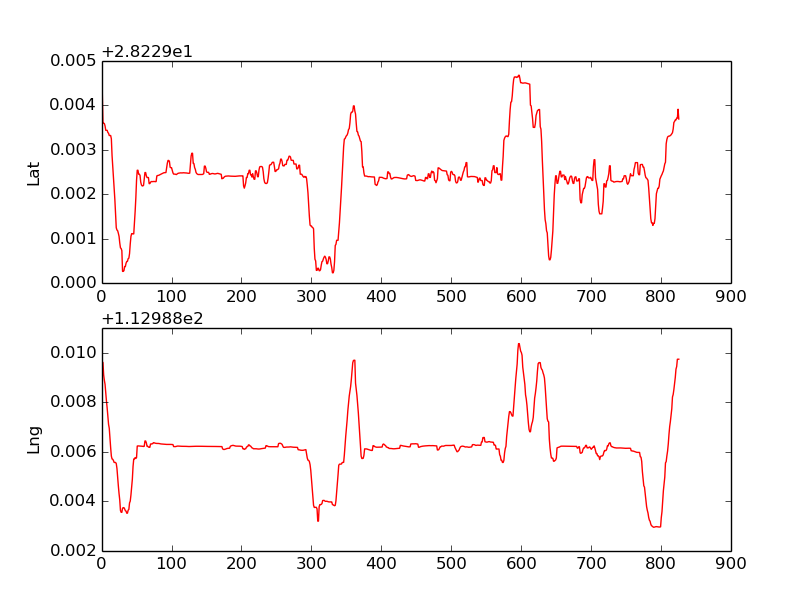
\includegraphics[height=4cm]{figure_4_mid_location2_kalman_ed}}
  \caption{卡尔曼滤波实验结果2}
  \label{fig:3_4_2}
\end{figure}
\par 在本研究中,我们采用了一种基于速度的分段卡尔曼滤波方法。考虑到在一个时间片内,如果当前位置点的速度和它之前的位置点的速度绝对差大于$\Delta v$ 时($\Delta v$作为一个未知的参数,需要我们在实际使用中给出)采用这样的方法将原有用户轨迹切分为$n$段然后针对每一段轨迹采用卡尔曼滤波算法,最终的部分轨迹滤波结果见图\ref{fig:3_5_1}、\ref{fig:3_5_2},可见经过按照速度分段后使用卡尔曼滤波能够比较好的过滤掉漂移点。
\begin{figure}[htb]
  \centering%
  \subfloat[原始轨迹数据]{%
    \label{fig:3_2_1_1}
    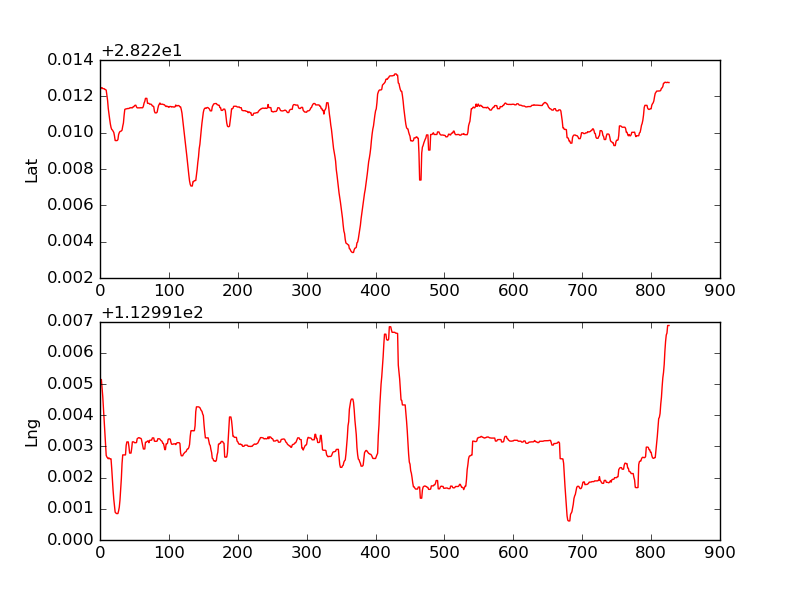
\includegraphics[height=4cm]{figure_4_mid_location1}}\hspace{4em}%
  \subfloat[分段卡尔曼滤波数据]{%
    \label{fig:3_2_2_1}
    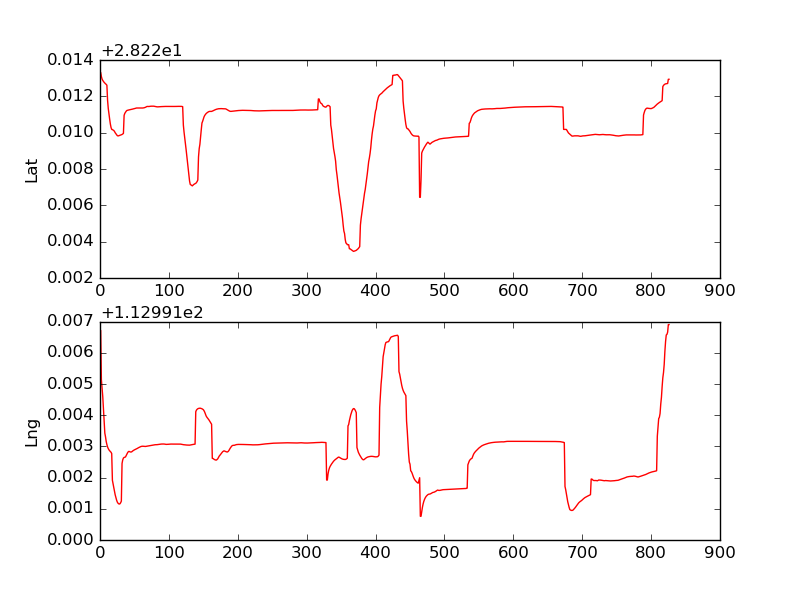
\includegraphics[height=4cm]{figure_4_mid_location1_kalman}}
  \caption{分段卡尔曼滤波轨迹结果1}
  \label{fig:3_5_1}
\end{figure}
\begin{figure}[htb]
  \centering%
  \subfloat[原始轨迹数据]{%
    \label{fig:3_2_2_1}
    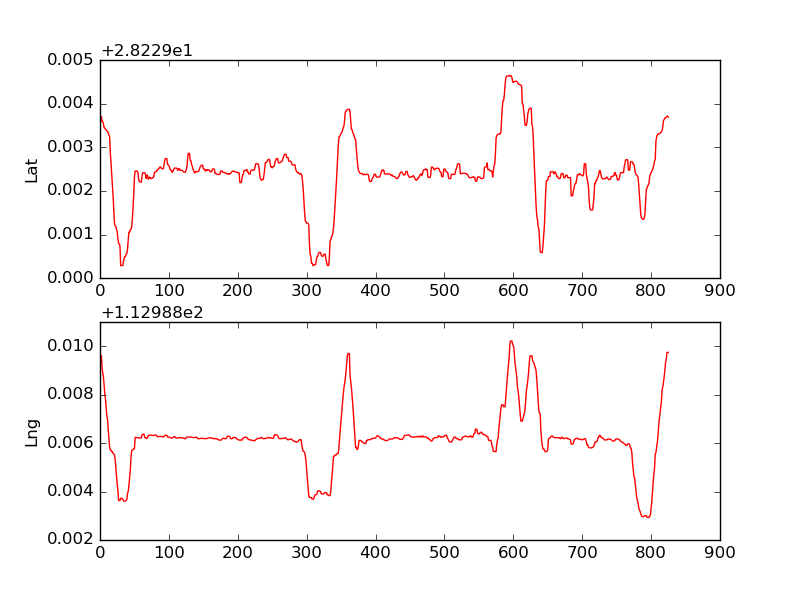
\includegraphics[height=4cm]{figure_4_mid_location2}}\hspace{4em}%
  \subfloat[分段卡尔曼滤波数据]{%
    \label{fig:3_2_2_2}
    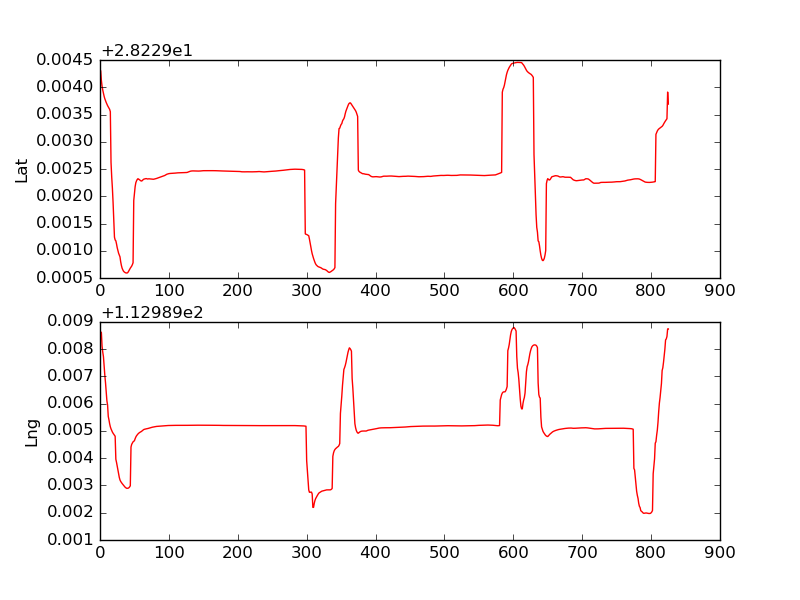
\includegraphics[height=4cm]{figure_4_mid_location2_kalman}}
  \caption{分段卡尔曼滤波轨迹结果2}
  \label{fig:3_5_2}
\end{figure}
\par 本小节主要针对前文中提及的三种常用的滤波算法进行了实验结果展示和效果分析,初步得出了使用卡尔曼滤波更加可行的判断结果。
\subsection{轨迹中停留点检测}
在实际生活中用户的轨迹是由一系列GPS点构成的,剔除其中的噪音点和用户在路上的点,能够从中挖掘出进一步信息的位置信息即为轨迹中的停留点,通常停留点并不是指用户轨迹中速度为零的点,而是由一组GPS 点构成区域,一个停留点通常对应现实生活中富有具体意义的点,能够更好的反映出用户之间轨迹的相似程度。如图\ref{fig:staypoint}所示,在现实生活中的停留点可以是一个具体的建筑名称,也可以是代表一个固定的区域,甚至可以是一个具有特殊意义的点。
\begin{figure}[htp]
\centering
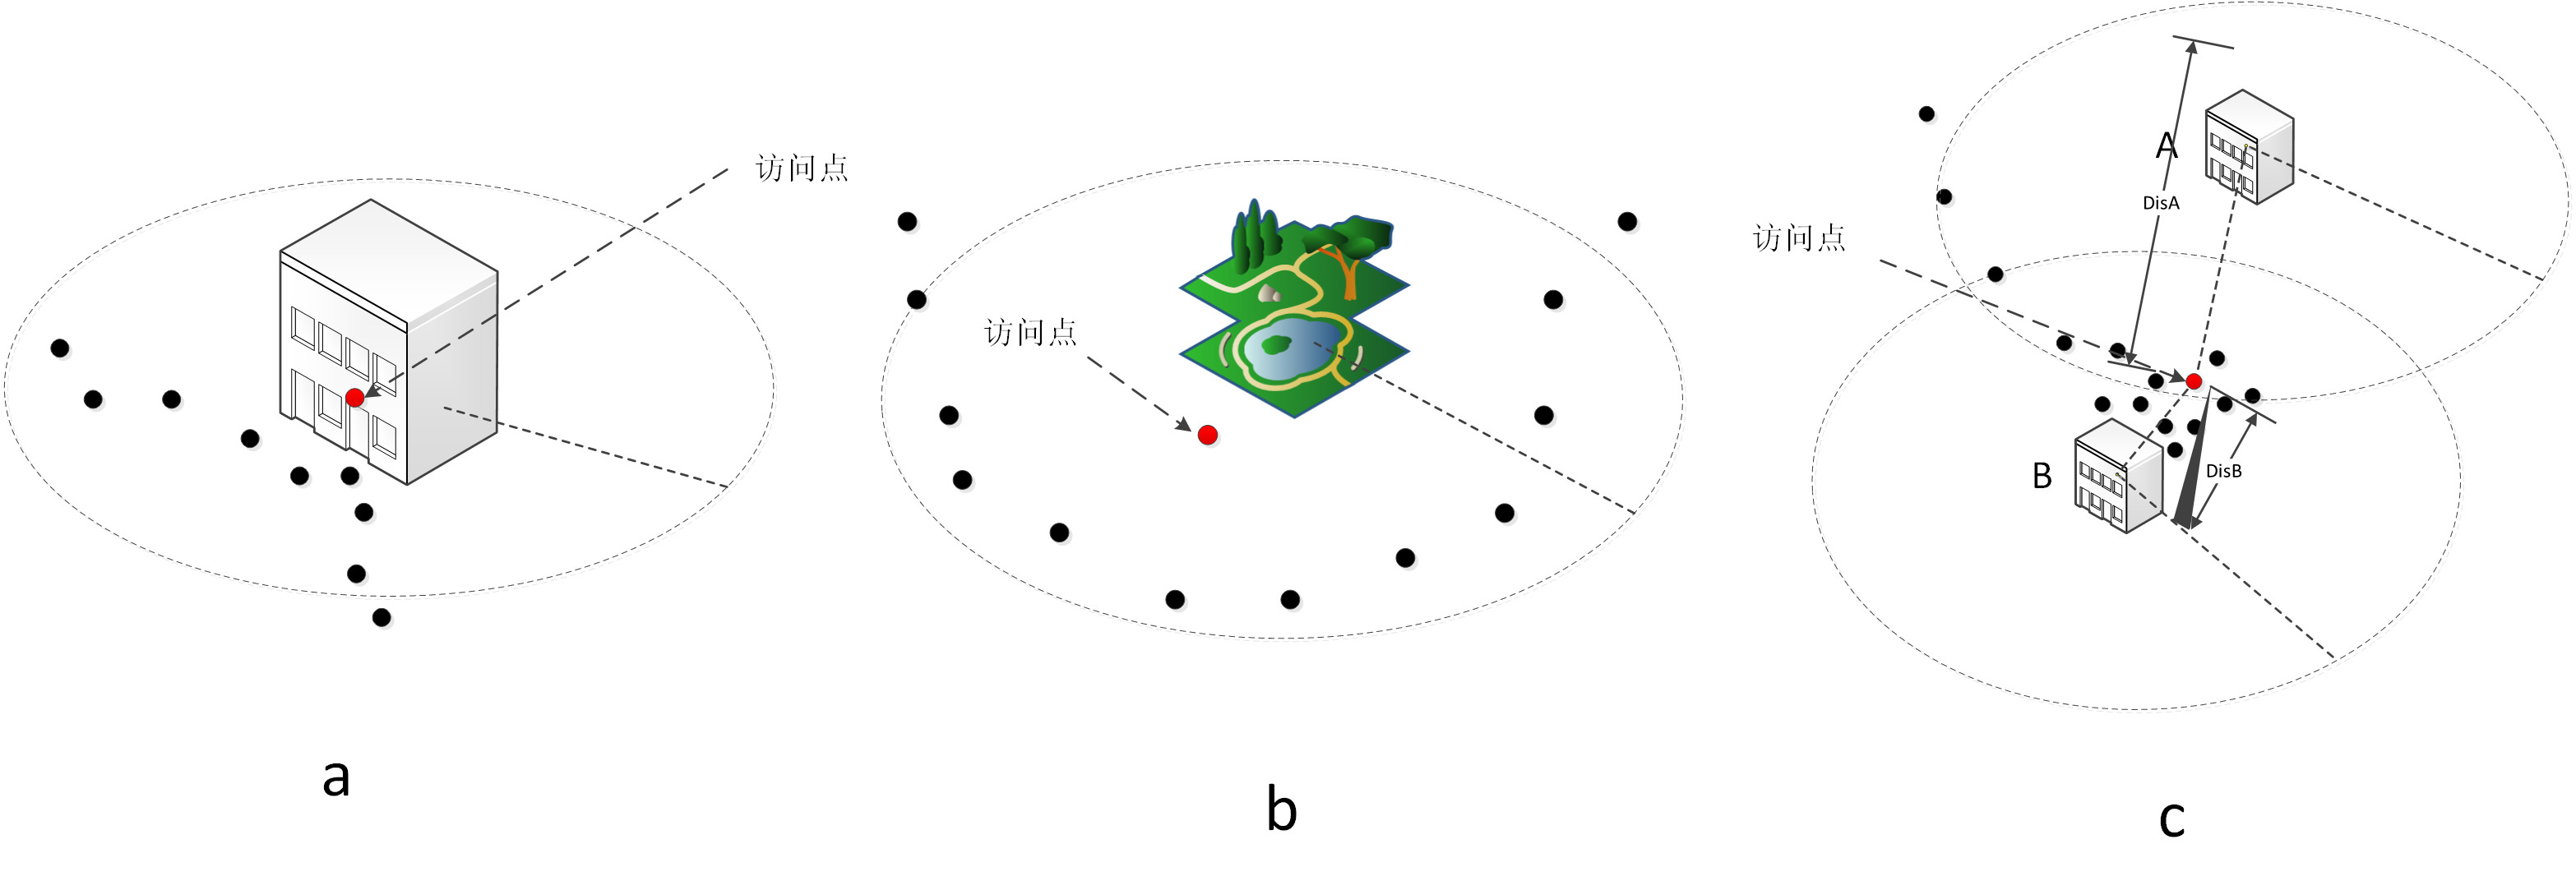
\includegraphics[width=0.8\textwidth]{figure_4_stay-points}
\caption{现实生活中的停留点示意图}
\label{fig:staypoint}
\end{figure}
\par 通过对停留点的识别,能够让我们更加深入的了解和认识用户的日常轨迹,同时从一个更加细粒度的层次来分析用户之间的轨迹相似度,停留点检测实验结果如图\ref{fig:SP_1}、\ref{fig:SP_2}所示,图中所得到的每一个停留点都具有丰富的现实意义,能够有效地表示用户访问的地点、位置。
\begin{figure}[htb]
  \centering%
  \subfloat[原始轨迹数据]{%
    \label{fig:3_3_1_1}
    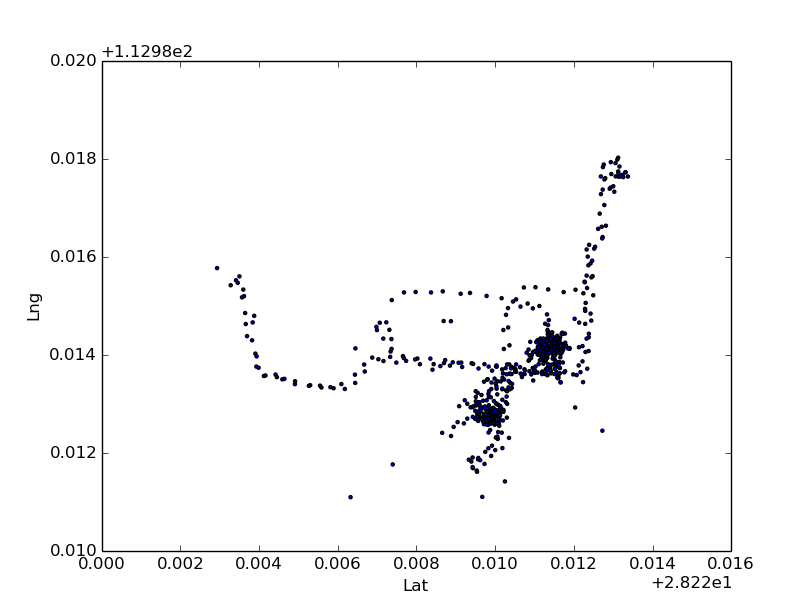
\includegraphics[height=4cm]{figure_4_location1_scater}}\hspace{4em}%
  \subfloat[检测出的停留点]{%
    \label{fig:sp_1}
    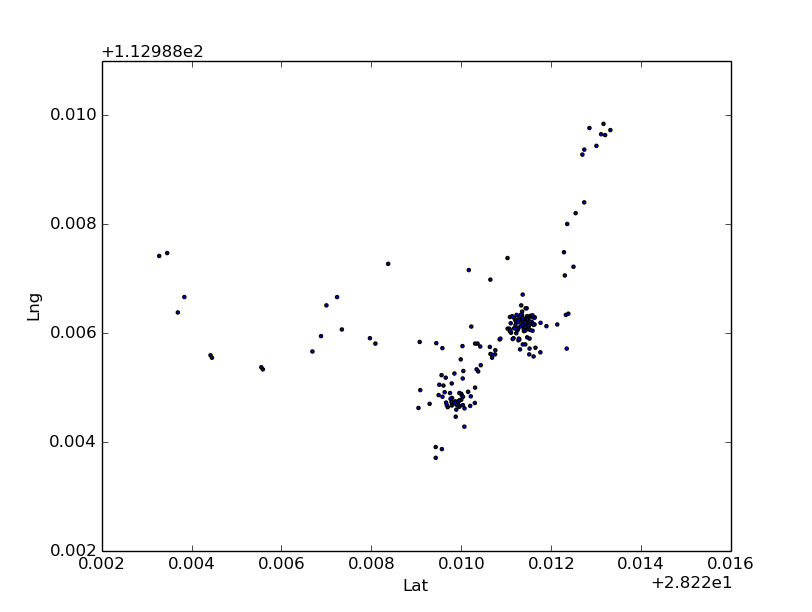
\includegraphics[height=4cm]{figure_4_location1_sp}}
  \caption{停留点检测实验结果1}
  \label{fig:SP_1}
\end{figure}
\begin{figure}[htb]
  \centering%
  \subfloat[原始轨迹数据]{%
    \label{fig:3_3_1_1}
    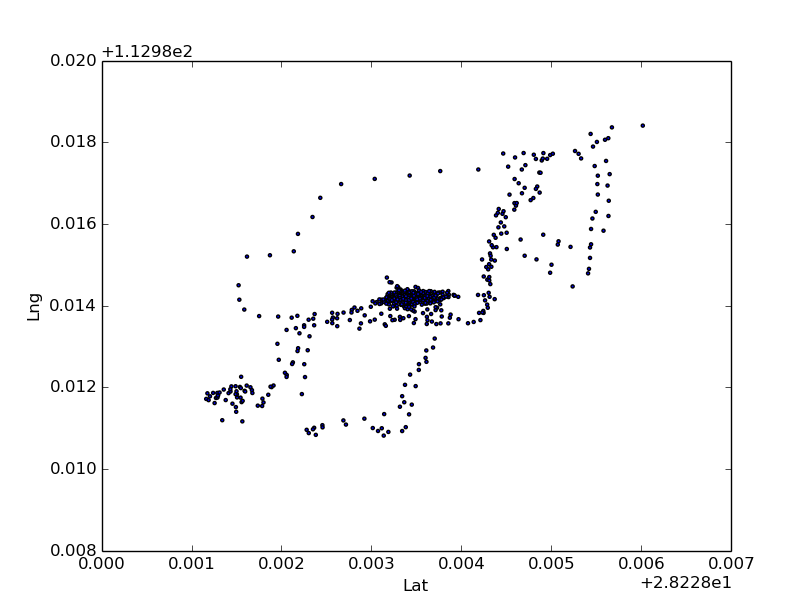
\includegraphics[height=4cm]{figure_4_location2_scater}}\hspace{4em}%
  \subfloat[检测出的停留点]{%
    \label{fig:sp_2}
    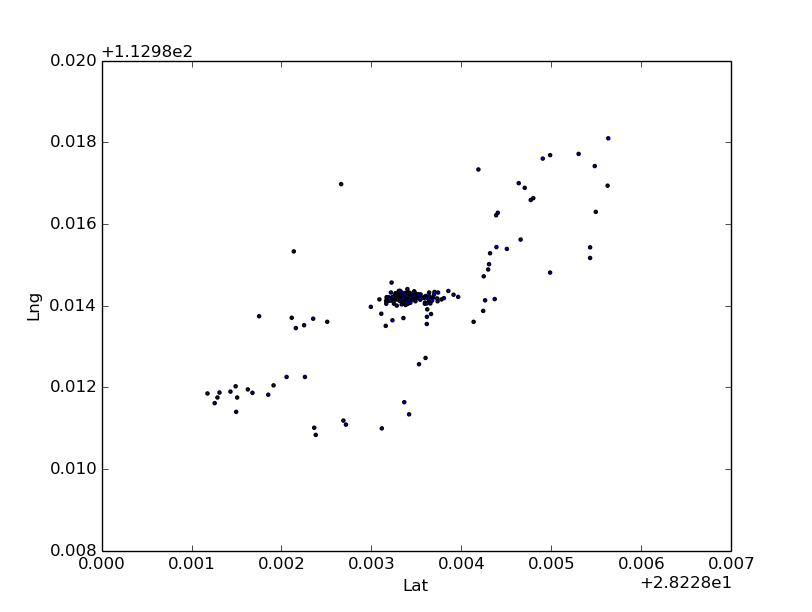
\includegraphics[height=4cm]{figure_4_location2_sp}}
  \caption{停留点检测实验结果2}
  \label{fig:SP_2}
\end{figure}
\subsection{用户轨迹停留点聚类}
\label{traclustar}
本节针对上面得到的用户轨迹中的停留点,采用不同的聚类算法所得到的不同的聚类结果进行描述。在前面的章节中我们详细介绍了聚类中常用的三种算法K-means聚类、DJ-Cluster的密度聚类和最新发表的改进的密度聚类算法,接下来我们将在实验中对这三种聚类算法进行比较。
\par 首先我们对用户轨迹数据采用K-means算法进行聚类实验,但是K-means聚类算法具有以下的明显的缺点:首先是K-means聚类结果依赖于参数$k$的初始化,其中$k$是指聚类个数。$k$个数的确定往往是靠经验值设定;其次是K-means算法初始化时聚类中心的选择,因为该算法采用的随机初始化聚类中心点,中心点选择不同会导致聚类的结果也出现差异甚至影响聚类的时间复杂度,使得聚类结果容易得到局部最优解而非全局最优解;最后的一个缺点是K-means聚类算法对原始数据中的噪音点和离群点非常敏感,聚类结果很容易受到离群点的影响从而导致簇的偏移。
\par 在本研究中因为是针对用户的空间轨迹进行聚类分析,而现实生活中用户的停留点主要是以相隔距离比较大的建筑等,因此在采用K-means聚类过程中,对噪音点的影响基本可以忽略不计,最主要的就是考虑不同的参数$k$对最终聚类结果的影响,图\ref{fig:3_8_1}、\ref{fig:3_8_2}主要展示不同的参数$k$取值对最终轨迹聚类结果的影响。图\ref{fig:3_9_1}、\ref{fig:3_9_2}在地图上标记了在不同参数$k$取值情况下的簇中心使得能够有更加直观的观察。
\begin{figure}[htb]
  \centering%
  \subfloat[原始轨迹数据]{%
    \label{fig:3_8_1_1}
    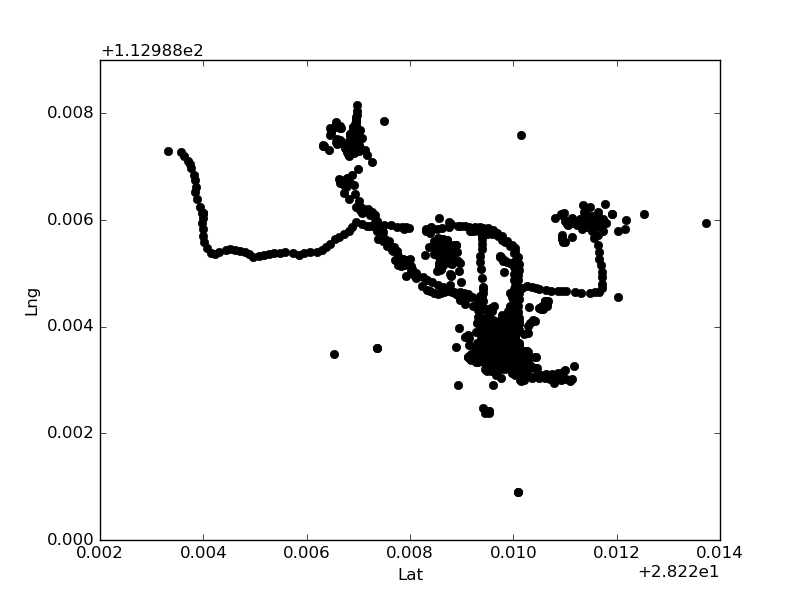
\includegraphics[height=5cm]{figure4_tra1}}%\hspace{4em}
  \subfloat[参数k=3]{%
    \label{fig:3_8_1_2}
    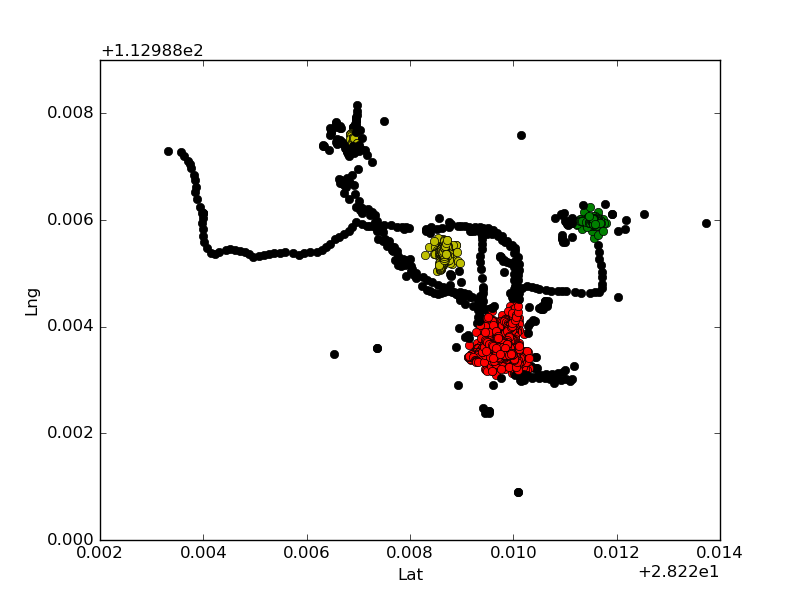
\includegraphics[height=5cm]{figure4_tra1_kmeans_3}}\\
  \subfloat[参数k=4]{%
    \label{fig:3_8_1_3}
    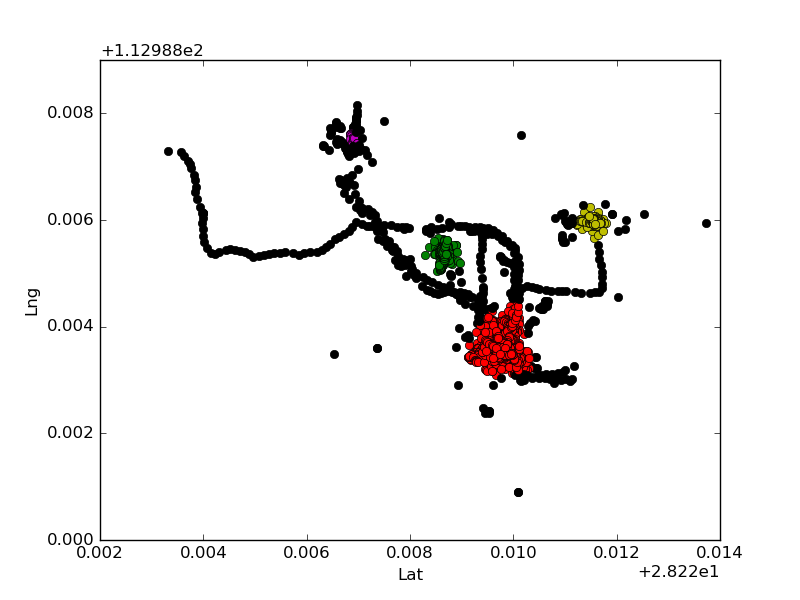
\includegraphics[height=5cm]{figure4_tra1_kmeans_4}}
  \subfloat[参数k=5]{%
    \label{fig:3_8_1_4}
    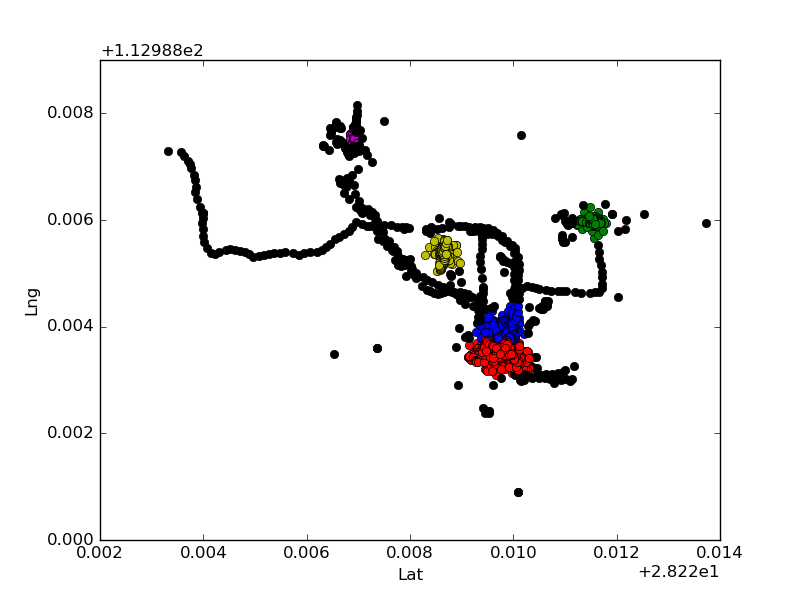
\includegraphics[height=5cm]{figure4_tra1_kmeans_5}}
  \caption{基于K-means的轨迹聚类实验结果1}
  \label{fig:3_8_1}
\end{figure}
\begin{figure}[htb]
  \centering%
  \subfloat[原始轨迹数据]{%
    \label{fig:3_9_1_1}
    \includegraphics[height=6cm]{figure4_tra1_map}}%\hspace{4em}
  \subfloat[参数k=3]{%
    \label{fig:3_9_1_2}
    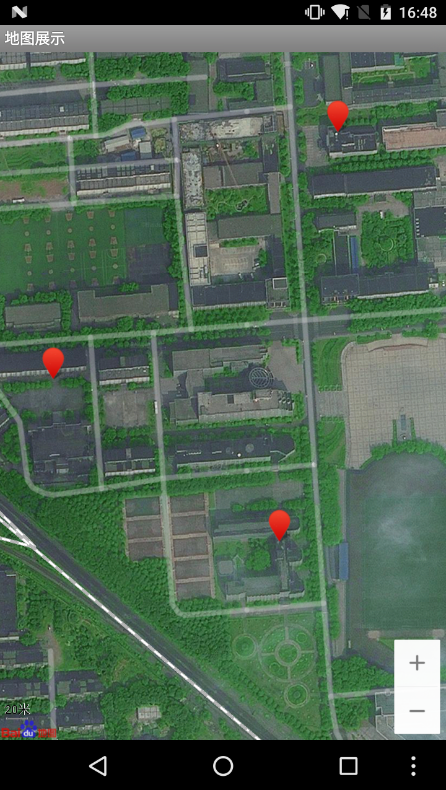
\includegraphics[height=6cm]{figure4_tra1_map_k3}}
  \subfloat[参数k=4]{%
    \label{fig:3_9_1_3}
    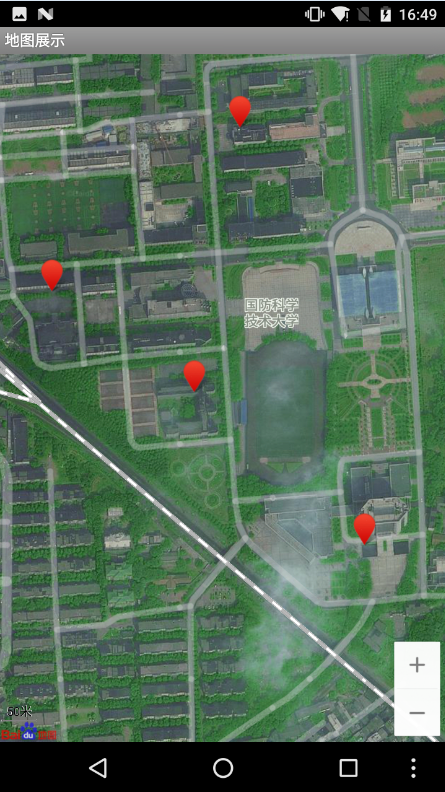
\includegraphics[height=6cm]{figure4_tra1_map_k4}}
  \subfloat[参数k=5]{%
    \label{fig:3_9_1_4}
    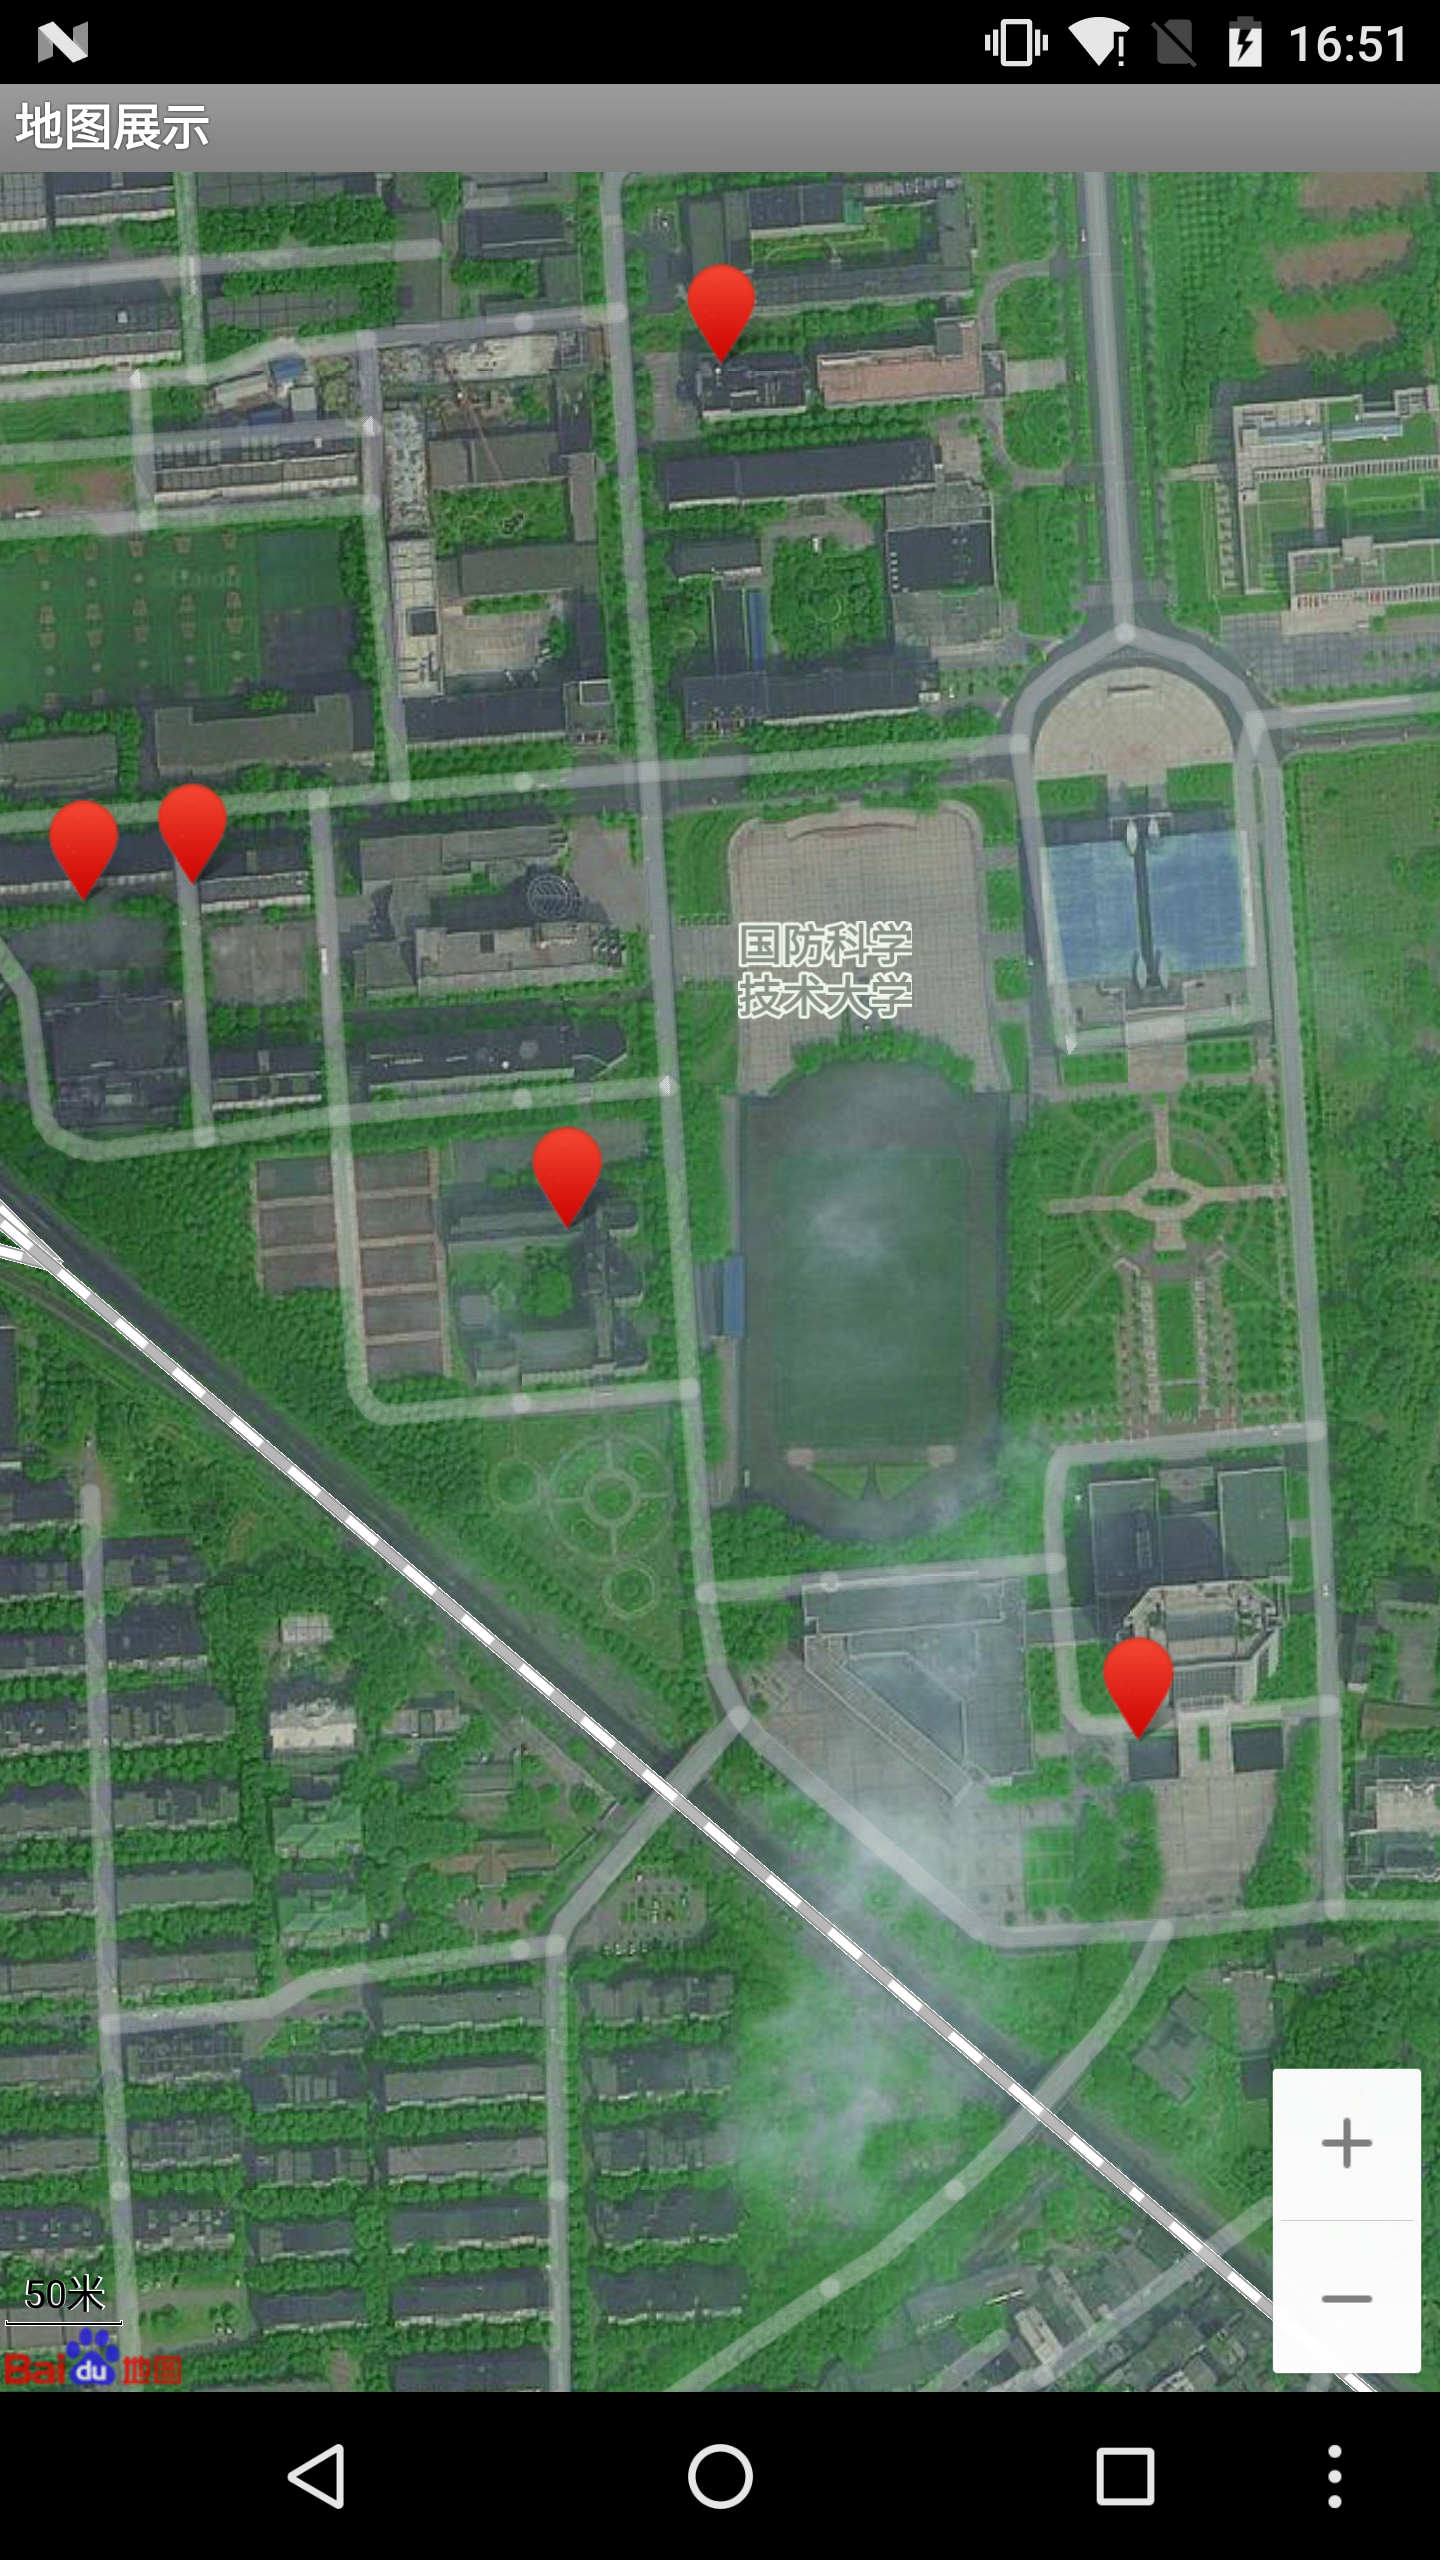
\includegraphics[height=6cm]{figure4_tra1_map_k5}}
  \caption{基于K-means的轨迹聚类实验结果地图展示1}
  \label{fig:3_9_1}
\end{figure}
\begin{figure}[htb]
  \centering%
  \subfloat[原始轨迹数据]{%
    \label{fig:3_8_2_1}
    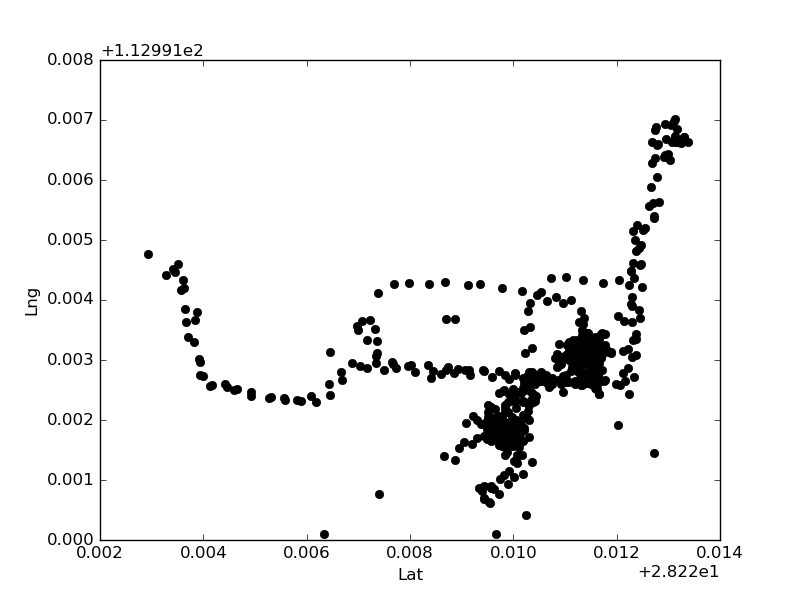
\includegraphics[height=5cm]{figure4_tra2}}%\hspace{4em}
  \subfloat[参数k=3]{%
    \label{fig:3_8_2_2}
    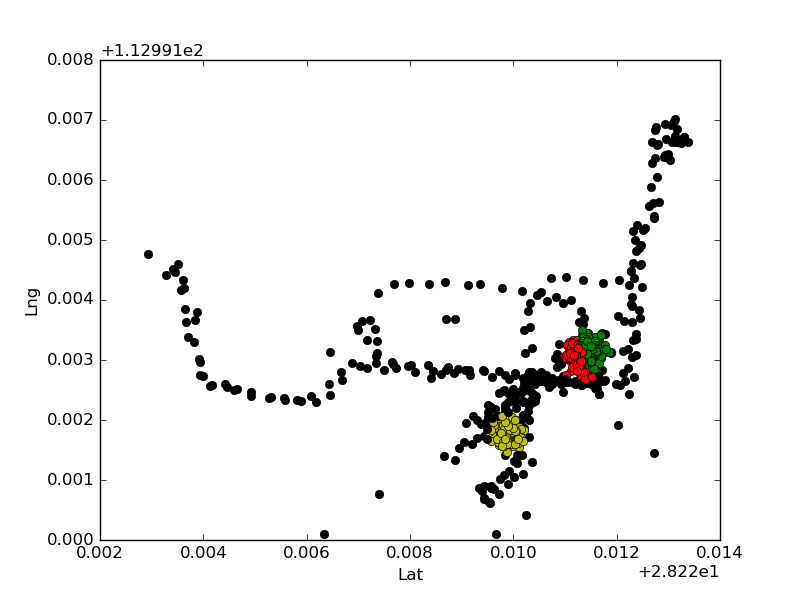
\includegraphics[height=5cm]{figure4_tra2_kmeans_3}}\\
  \subfloat[参数k=4]{%
    \label{fig:3_8_2_3}
    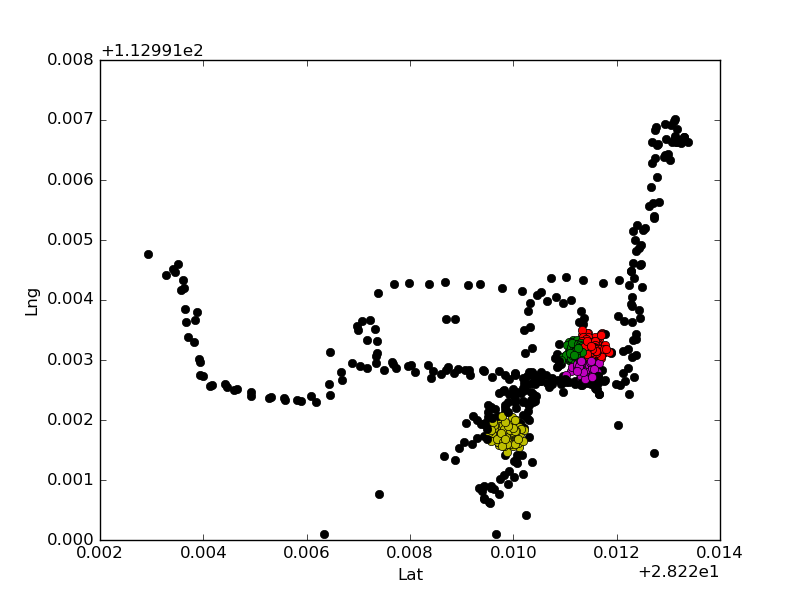
\includegraphics[height=5cm]{figure4_tra2_kmeans_4}}
  \subfloat[参数k=5]{%
    \label{fig:3_8_2_4}
    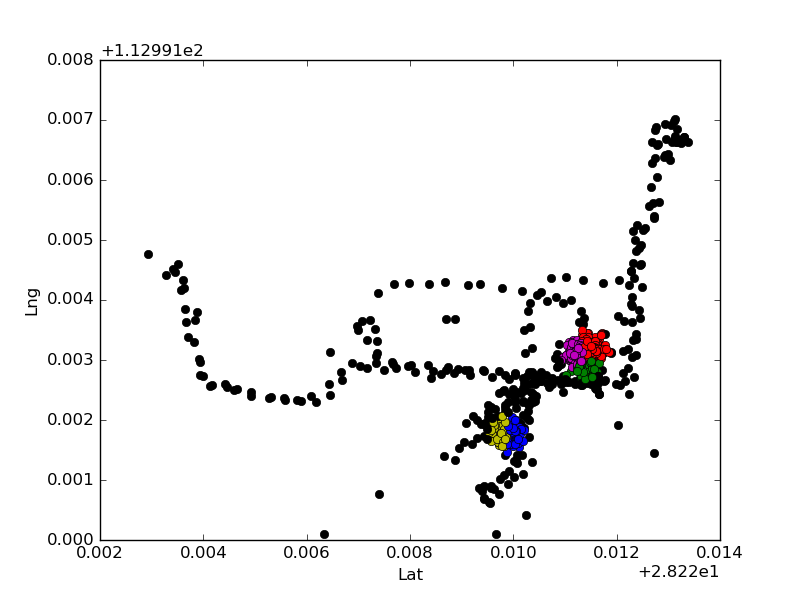
\includegraphics[height=5cm]{figure4_tra2_kmeans_5}}
  \caption{基于K-means的轨迹聚类实验结果2}
  \label{fig:3_8_2}
\end{figure}
\begin{figure}[htb]
  \centering%
  \subfloat[原始轨迹数据]{%
    \label{fig:3_9_2_1}
    \includegraphics[height=6cm]{figure4_tra2_map}}%\hspace{4em}
  \subfloat[参数k=3]{%
    \label{fig:3_9_2_2}
    \includegraphics[height=6cm]{figure4_tra2_map_k3}}
  \subfloat[参数k=4]{%
    \label{fig:3_9_2_3}
    \includegraphics[height=6cm]{figure4_tra2_map_k4}}
  \subfloat[参数k=5]{%
    \label{fig:3_9_2_4}
    \includegraphics[height=6cm]{figure4_tra2_map_k5}}
  \caption{基于K-means的轨迹聚类实验结果地图展示2}
  \label{fig:3_9_2}
\end{figure}
\par 通过对轨迹数据的聚类分析我们可以得知,如果在聚类前我们能够确切的知道用户的轨迹数据应该划分的簇的个数,那么K-means聚类算法将会得出非常合理的结果,我们在观察图\ref{fig:3_9_1}、\ref{fig:3_9_2}时发现,当簇的个数越接近符合用户访问位置个数的时候,那么聚类点将更能够反映出真实的情况,在图\ref{fig:3_11_1}中,(a)所对应的聚类得到的簇包含了实际上没有正确的将用户访问过的位置区分开,因为这两个访问的位置距离相隔太近,导致K-means算法将这两个簇合并为一个簇,但是如果我们将聚类个数设置为5就能够成功的识别出这两个位置。在另一实验结果图\ref{fig:3_11_2}中也出现了类似的情况。但是根据图中实验情况分析发现对于一部分在路上的点被划分到了聚类簇中,同时有些应该被单独聚类成一个独立的簇的点被划分到了在路上的点中,这些都是因为我们无法正确的给出符合当前轨迹访问点个数的聚类个数所造成的。
\par 接下来将会基于DJ-Cluster 算法来对轨迹数据进行聚类并对结果进行分析。DJ-Cluster算法是基于密度聚类算法DBSCAN而改进的一种密度聚类算法,通过利用密度相连的原理可以发现任意形状的簇,但是算法存在有一个局限性:算法的性能和准确性依赖于参数$Eps$(邻域半径)和$MinPts$(最少点数量),如果邻域半径的取值过大那么所有的点将会划分为同一个簇,因此在实际的使用过程中,需要不断地对参数进行调整才能得到比较理想的结果,如图\ref{fig:3_10_1}、\ref{fig:3_10_2}结果所示,实际地图中结果展示如图\ref{fig:3_11_1}、\ref{fig:3_11_2}所示。
\begin{figure}[htb]
  \centering%
  \subfloat[原始轨迹数据]{%
    \label{fig:3_10_1_1}
    \includegraphics[height=4cm]{figure4_tra_for_dj_1}}\hspace{4em}%
  \subfloat[DJ-Cluster聚类结果]{%
    \label{fig:3_10_1_2}
    \includegraphics[height=4cm]{figure4_tra_result_dj_1}}
  \caption{基于DJ-Cluster的轨迹聚类实验结果1}
  \label{fig:3_10_1}
\end{figure}
\begin{figure}[htb]
  \centering%
  \subfloat[原始轨迹数据]{%
    \label{fig:3_11_1_1}
    \includegraphics[height=6cm]{figure4_tra_map_dj1}}\hspace{4em}%
  \subfloat[DJ-Cluster聚类结果]{%
    \label{fig:3_11_1_2}
    \includegraphics[height=6cm]{figure4_tra_map_result_dj_1}}
  \caption{基于DJ-Cluster的轨迹聚类实验结果地图展示1}
  \label{fig:3_11_1}
\end{figure}
\begin{figure}[htb]
  \centering%
  \subfloat[原始轨迹数据]{%
    \label{fig:3_10_2_1}
    \includegraphics[height=4cm]{figure4_tra_for_dj_2}}\hspace{4em}%
  \subfloat[DJ-Cluster聚类结果]{%
    \label{fig:3_10_2_2}
    \includegraphics[height=4cm]{figure4_tra_result_dj_2}}
  \caption{基于DJ-Cluster的轨迹聚类实验结果2}
  \label{fig:3_10_2}
\end{figure}
\begin{figure}[htb]
  \centering%
  \subfloat[原始轨迹数据]{%
    \label{fig:3_11_2_1}
    \includegraphics[height=6cm]{figure4_tra_map_dj2}}\hspace{4em}%
  \subfloat[DJ-Cluster聚类结果]{%
    \label{fig:3_11_2_2}
    \includegraphics[height=6cm]{figure4_tra_map_result_dj_2}}
  \caption{基于DJ-Cluster的轨迹聚类实验结果地图展示2}
  \label{fig:3_11_2}
\end{figure}
\par 通过观察结果地图展示和原始数据对比能够发现,相比于K-means算法DJ-Cluster能够得到比较正确的结果,但是结果依赖于对前面所描述的参数的不断调整。从图\ref{fig:3_11_1}中(a)中描绘的用户位置点集合(b)中得到的聚类结果进行分析,右上角是宿舍区域,因为当前点比较少,未能够正确的将这个区域聚类成一个单独的簇进行标记。但是从图\ref{fig:3_11_2}中发现DJ-Cluster基本得到了非常好的聚类结果。受限于DJ-Cluster算法对参数的敏感性,接下来将介绍一种新的聚类算法,该算法将大大降低对参数和数据的依赖性。
\par 接下来进一步展示在Science上发表的聚类算法,该算法通过结合现实理论,假设聚类的中心实质上是有局部密度低的点所环绕的,并且这点和另外密度高的点距离都比较大。这样通过计算得到每个点的当前密度值后根据划分的边界阈值进行密度点的划分,找出每个块中密度最大的点并将其周围密度小于该点密度的点加入到当前簇中得到最终的聚类结果。该算法因为考虑当将点密度排序后进行处理,保持了点密度顺序的相对稳定的同时减小了半径阈值带来的影响。聚类算法的具体的实验结果见图\ref{fig:3_12_1}、\ref{fig:3_12_2},将聚类结果通过地图展示如图\ref{fig:3_13_1}、\ref{fig:3_13_2}所示,从图\ref{fig:3_12_1}中可以观察到聚类结果是比较
\begin{figure}[htb]
  \centering%
  \subfloat[原始轨迹数据]{%
    \label{fig:3_12_1_1}
    \includegraphics[height=4cm]{figure4_tra_for_science1}}\hspace{4em}%
  \subfloat[聚类结果]{%
    \label{fig:3_12_1_2}
    \includegraphics[height=4cm]{figure4_science_1_cluster}}
  \caption{轨迹聚类实验结果展示1}
  \label{fig:3_12_1}
\end{figure}
\begin{figure}[htb]
  \centering%
  \subfloat[原始轨迹数据]{%
    \label{fig:3_13_1_1}
    \includegraphics[height=6cm]{figure4_tra_map_science1}}\hspace{4em}%
  \subfloat[聚类结果]{%
    \label{fig:3_13_1_2}
    \includegraphics[height=6cm]{figure4_tra_map_result_science1}}
  \caption{轨迹聚类实验结果地图表示1}
  \label{fig:3_13_1}
\end{figure}
\begin{figure}[htb]
  \centering%
  \subfloat[原始轨迹数据]{%
    \label{fig:3_12_2_1}
    \includegraphics[height=4cm]{figure4_tra_for_science2}}\hspace{4em}%
  \subfloat[聚类结果]{%
    \label{fig:3_12_2_2}
    \includegraphics[height=4cm]{figure4_science_2_cluster}}
  \caption{轨迹聚类实验结果展示2}
  \label{fig:3_12_2}
\end{figure}
\begin{figure}[htb]
  \centering%
  \subfloat[原始轨迹数据]{%
    \label{fig:3_13_2_1}
    \includegraphics[height=6cm]{figure4_tra_map_science2}}\hspace{4em}%
  \subfloat[聚类结果]{%
    \label{fig:3_13_2_2}
    \includegraphics[height=6cm]{figure4_tra_map_result_science2}}
  \caption{轨迹聚类实验结果地图表示2}
  \label{fig:3_13_2}
\end{figure}
\par 通过分析图\ref{fig:3_12_1}和图\ref{fig:3_12_1}中的聚类结果发现该聚类算法能够比较正确的将用户的轨迹数据进行聚类同时也不依赖于太敏感的参数输入。在图\ref{fig:3_12_1}中用户正确访问的地方应该是五个,虽然(b)中的聚类结果也得出了五个簇中心位置,但是未能将寝室这一簇识别出来而是将在体育馆周围的点标注为聚类簇。虽然在最终的结果上有的会出现一点误差,但是能够去除对数据和参数的敏感性减少对实验的干预,在本研究中显得更加难能可贵和适用。
%\par 通过以上的实验方法,我们在得到用户的停留点和聚类轨迹之后,将会采用语义标签数据库和反地理编码查询相结合的手段进行轨迹语义化处理,假设得到了用户一天的轨迹数据并且进行了停留点切分和聚类得到了100个位置,而我们的语义标签数据库中只能够查询到其中的70个位置的语义标签,因此剩下的30个位置我们将采用反地理编码进行语义化,并将相对于的语义标签存入到语义数据库中避免二次调用反地理编码接口。
\par 本小节主要讨论了前面一章节中介绍的聚类算法在本研究中对用户轨迹聚类的效果以及每种聚类算法对参数的依赖以及影响,然后分析每一种聚类算法各自的优缺点,K-means聚类结果虽然比较好但是需要预先设定聚类个数,最明显的问题是我们收集的用户轨迹数据中无法预先知晓用户轨迹所应该聚类的个数,导致结果出现偏差;DJ-Cluster聚类算法同样存在类似的问题。本课题采用针对小数据进行聚类,一方面是因为数据量小比较容易发现较小的聚类簇,能够识别用户更加细粒度的访问位置,如果将用户多天的轨迹数据进行聚类,有可能将会导致较大数量的簇无法识别。另外采用小数据量时间切片进行分析聚类能够保证当前用户的某个聚类没有识别而下一段数据分析识别出来,形成效果叠加也能够保证最终结果的相对稳定,下一节将简要讨论如何对用户的轨迹点进行语义化。
\subsection{对用户轨迹的语义位置添加语义标签}
\label{sec:section3-3}
\par 在上面的小节中主要讲述了针对用户原始GPS轨迹数据进行滤波处理、轨迹停留点挖掘以及针对用户轨迹进行聚类。但是仅仅得到用户的空间轨迹信息是不够的,为此我们需要将用户轨迹中有意义的点添加上语义标签如图\ref{fig:tra_senantic}所示,为用户轨迹中的停留点加上语义标签,得能有助于我们了解用户去了什么地方,这些地方属于什么类型等。语义轨迹有助于我们进一步分析用户之间的相似性,因此本小节将介绍如何添加语义轨迹。
\par 现有的大多数工作是基于反地理编码技术来将空间轨迹语义化,将用户的位置转换为具体的道路门牌号等(如德雅路138号),然而有时候道路地址无法有效地表示用户位置的现实意义;另外的方法采用了机器学习的方法,首选从用户的轨迹中提取用户的位置点以及位置点的类型,采用关系马尔科夫网模型,利用网中的节点表示用户的访问点,基于条件随机场对用户的访问点进行推测得到用户的访问点的语义标签,但是采用机器学习效率较低,同时最终结果还受限于数据训练集,不适合普适计算的要求。因此我们采用了以语义标签数据库为主,反地理编码为辅的语义化方法。语义标签数据库中覆盖了本研究对象校园内部及其周边大部分语义位置点,假设得到了用户一天的轨迹数据并且进行了停留点切分和聚类得到了100个位置,而我们的语义标签数据库中只能够查询到其中的70个位置的语义标签,因此剩下的30个位置我们将采用反地理编码进行语义化,并将相对于的语义标签存入到语义数据库中避免二次调用反地理编码接口。如图\ref{fig:tra_senantic}所示,我们采用了三层了轨迹语义化处理模型,在最底层为用户的原始轨迹数据,中间层为上一小节中我们识别出的用户停留点或者聚类簇,最上层为用户的访问地点语义标签。
\begin{figure}[htp]
\centering
\includegraphics[width=0.8\textwidth]{figure_4_stay-point_semantic}
\caption{位置语义标签示意图}
\label{fig:tra_senantic}
\end{figure}
\par 在语义化的过程中,我们首先构建了一个符合当前范围内的语义标签数据库,里面包含了学校内部各个位置语义点以及学校周边大部分的位置语义信息,在为用户轨迹添加语义标签时,首先查找语义标签数据库内是否有相匹配的位置点。具体的匹配过程如图\ref{fig:matchlabel}所示,图中首先我们需要人为设定一个距离阈值,用来衡量当前位置点与语义标签位置点之间的关系。图\ref{fig:matchlabel}中a所示:当停留点或簇中心点距离语义标签库中有且仅有一个位置点的距离小于设定的阈值,则把当前语义标签赋予给当前位置;若如图\ref{fig:matchlabel}中b所示,当半径阈值内不止一个符合要求的语义标签点时,我们选择和当前位置点距离最近的语义标签作为当前位置点的标签;当语义标签数据库中无法查询到与当前位置相匹配的标签点时,将会调用反地理编码,获取到当前位置的语义标签,结果示意图如图\ref{fig:map_label}所示,在图\ref{fig:map_label}(a)和(b)中,因为这两处地理位置的语义标签都已经存在于语义标签数据库中,所以查询时就返回数据库中的标签,而(c)中的位置因为暂时没有保存在标签数据库中,因此调用百度地图API将得到的中心点坐标转换为百度地图数据库中的标注地址并将结果返回和保存。
\begin{figure}[htp]
\centering
\includegraphics[width=0.8\textwidth]{figure4_matchlabel}
\caption{语义标签识别示意图}
\label{fig:matchlabel}
\end{figure}

\begin{figure}[htb]
  \centering%
  \subfloat[语义标签数据库标签示意图1]{%
    \label{fig:label1}
    \includegraphics[height=6cm]{figure4_map_label1}}\hspace{4em}%
  \subfloat[语义标签数据库标签示意图2]{%
    \label{fig:label2}
    \includegraphics[height=6cm]{figure4_map_label2}}\hspace{4em}%
  \subfloat[反地理编码标签示意图]{%
    \label{fig:label3}
    \includegraphics[height=6cm]{figure4_map_label3}}
  \caption{语义标签结果示意图}
  \label{fig:map_label}

\end{figure}
\par 在用户轨迹语义化的过程中还存在以下这样的问题:第一不同用户或者同一个用户访问同一个语义位置(如食堂、学生宿舍)等的时候,由于手机设备不同和GPS数据采样的误差,导致用户当前停留位置的聚类中心并不一定和数据库中记载的完全相同,因此我们在查询语义数据库的时候,需要设定一个中心点距离阈值比如说15米,如果当前中心点位置和其中某一个标签的位置距离小于15米,就将该语义标签赋予当前中心点;如果同时落入了多个语义点的半径范围内,则将距离最近的语义中心点的标签赋予给当前中心点。
\par 另外一个问题是由第一个问题引申而来即半径阈值的取值为多少才能给既准确的识别中心点语义标签又能给使得临近语义点的距离足够大,这样才能有效的对轨迹停留点进行语义标注,在实验过程中发现基于小样本数据在小范围内(如整个校园内及其周围)的语义标签化得到的数据相对于可靠,可能是由于在小范围内的GIS语义标签数据库比较完备,能够有效地识别出用户大部分的停留点。但是如果将数据进一步增加,将活动范围扩大,那么这种方法的可靠性和得到的语义标签的准确性也将受到影响。如果能够得到一个大区域内的GIS信息库或者是人工标注好这样的语义标签库,那么就能够应对这样的问题,但是这样显得缺乏可行性,如何针对在大区域内的语义轨迹化也是我们未来工作的研究之一。
\section{用户GPS轨迹数据结构化表示}
\label{sec:section3-4}
通过前面章节的停留点检测算法以及实践,能够得到用户轨迹中存在的停留点,接下来我们要构建一个用户表示用户轨迹的模型,针对每个用户利用轨迹表示模型来描述和存储该用户所有时间内的轨迹信息。为了便于在下面章节中对基于空间轨迹的用户关系强度度量,我们采用了一种基于三维的层次化的GPS轨迹表示模型来描述用户在纵向时间维度内以及横向空间维度中的活动。如图\ref{fig:tramodel}所示,在此抽象表示结构中,其中第一维表示用户维度,第二维的每一行表示用户在当前日期内所有的轨迹集合,第三维中的每一列表示用户在当前日期内,按照时间分割后的时间片中所有的停留点集合,最后得到的结果中$Gtra_{i}$表示用户$U_{i}$所有的轨迹集合。
\par 根据前面章节中获取的用户位置信息多为一个经纬度点的集合或一个几何形状,没有包含任何可以直接识别的信息。通过轨迹语义化,我们基于用户的GPS轨迹得到了用户的语义位置轨迹。不同于用户地理轨迹的抽象表示方法,用户的语义轨迹表示更加具有难度和挑战性,根据前面的描述得知:现实生活中同一个用户多次访问同一语义位置所产生的空间位置停留点可能不相同(GPS定位存在偏移),直接对停留点进行语义化并不可行,因此我们在节\ref{traclustar}中针对部分停留点进行聚类得到用户的轨迹中停留点的聚类簇,然后用当前的结果替换原有轨迹中对应的停留点。如图\ref{fig:semantic_model}所示,我们首先从用户GPS轨迹数据中抽象出表示用户空间地理位置的空间轨迹数据结构;然后将聚类后得到的停留点簇按照节\ref{sec:section3-3}对停留点添加语义标签得到用户的语义轨迹。现实生活中,人们日常轨迹中的位置移动常常表现为从一个位置移动到另一个位置(如早上从寝室步行到食堂再去图书馆等),在图\ref{fig:semantic_model}中我们借鉴这样的想法将用户每天的GPS运动轨迹向量序列化后的结果赋值为用户的轨迹向量,再根据时间戳信息结合语义标签构建用户的语义轨迹时间向量,得到用户在一段时间片内的语义轨迹向量,最后将每天的轨迹向量合并得到用户的语义轨迹序列描述,通过对这种语义轨迹的结构化表示,可以有效地将空间轨迹转换为用户的日常语义轨迹,便于下一步计算用户之间的关系强度。
\begin{figure}[htp]
\centering
\includegraphics[width=0.8\textwidth]{figure4_tra_model}
\caption{用户轨迹的抽象表示}
\label{fig:tramodel}
\end{figure}
\begin{figure}[htp]
\centering
\includegraphics[height=7.5cm,width=0.7\textwidth]{figure4_semantic_model}
\caption{用户语义轨迹描述模型}
\label{fig:semantic_model}
\end{figure}
\par 在获得用户的语义轨迹之后我们将用户的语义轨迹序列按照时间片进行划分,得到形如$\left \{Sloc_{1},Sloc_{2},\cdots ,Sloc_{n} \right \}$ 结构的用户语义轨迹序列集合,最终得到的语义轨迹结构如图\ref{fig:tra_semantic_model}中的示例描述。
\begin{figure}[htp]
\centering
\includegraphics[width=0.8\textwidth]{figure4_tra_semantic_model}
\caption{语义轨迹示意图}
\label{fig:tra_semantic_model}
\end{figure}
\par 从用户的历史轨迹数据中所挖掘出的频繁模式和序列模式能够反映出用户的日常轨迹运动习惯和行为规律,运动模式在现实生活中表现为用户经常行走的路径序列,是用户轨迹数据规律的抽象表示。用户的日常运动模式在一定程度上代表了用户的个人喜好、意图以及活动模式,例如用户A经常下午去操场跑步,B周末经常去市区逛街等,当从一个更细的粒度甚至能够根据用户的用餐地点推测出用户的口味喜好等。本文首先采用频繁模式和序列模式挖掘算法来探寻用户的日常轨迹运动模式,最后得到用户的运动模式矩阵,矩阵中的行$$TraFP_{i,j,k}=\left \{  (Sloc_{1}),(Sloc_{2}, \cdots ,Sloc_{m})\cdots   \right \}$$ 表示用户$u_{i}$在时间周期$k$内的日常语义轨迹中所挖掘出的频繁模式的第$j$项纪录;而$$TraSQ_{i,j,k}=\left \{  <Sloc_{1}>,<Sloc_{2}, \cdots ,Sloc_{n}>\cdots   \right \} $$表示用户$u_{i}$在时间周期$k$内的日常语义轨迹中所挖掘出的系列模式的第$j$项纪录,这些都将会在下一章中进行详细的描写如何利用用户轨迹运动模式来计算用户之间的关系强度。
\section{WiFi感知数据处理计算技术}
\label{wifi_pro_tec}
在日常生活中WiFi的感知距离因为受到发射器功率以及周围环境的影响,导致正常WiFi的覆盖范围大约在20米左右。当用户处在不用的上下文环境中时其周围能够被StarLog所感知到的WiFi环境也是不同的,不仅如此,对于一个很小的范围内(如教室、图书馆、办公室等)的WiFi上下文环境基本是极度相似的甚至相同的,也就是说能够探明检测到的WiFi列表应该是相同的,因此我们根据WiFi感知数据的这一特性来计算用户之间的关系强度。根据图\ref{fig:7_1_wifi}中的处理流程描述,首选我们将原始WiFi感知数据进行处理,从中提取出有用的数据信息(如WiFi接入名称、WiFi强度、WiFi接入点的MAC地址、扫描时间等);其次在提取出的数据的基础之上,我们根据探测的时间戳信息,将WiFi数据序列化。如图\ref{fig:wifimodel_process}所示,我们采用矩阵的方式来表示所有用户在整个数据收集期间的WiFi序列集合,其中每一行表示实验数据收集的时间维度从第一天到第N天;每一列代表一个独立的用户,其中$[i,j]$表示用户$u_{j}$在第$i$天的的WiFi向量数据。每一条WiFi向量数据都是由许多切片时间内的WiFi 上下文(WiFi context)所构成的。
\begin{figure}[htp]
\centering
\includegraphics[width=0.8\textwidth]{figure4_wifimodel}
\caption{WiFi数据结构化表示示意图}
\label{fig:wifimodel_process}
\end{figure}
\par 每一次所感知的WiFi上下文环境信息是不仅包含了WiFi连接名,还包含了接入点MAC地址、信号强度、设备类型等复杂的信息,如图\ref{fig:wifi_context}所示,WiFi-context更形象的描述是当前WiFi数据收集时刻时,设备周围的感知信息和环境信息,本课题转换视角将WiFi感知序列拟物化,看做我们现实中生活的环境,考虑到当用户1当前时刻所处的环境和用户2所处的环境极度相似或者相同的时候,那么我们就认为二者在同一个环境中也就是产生了现实交互比没有在同一环境中的用户具有更强的关系强度。因此我们将当前时刻的环境用无向带权图来表示,即假设每一个能够探知的WiFi源都与设备存在一条边,然后用户在一段时间内的数据就成了一张图如图\ref{fig:wifi_context_graph},最后比较两个用户的在每一个时间切片下的图的相似性推断出用户的关系强度。
\begin{figure}[htp]
\centering
\includegraphics[width=0.7\textwidth]{figure4_wifi_context}
\caption{WiFi上下文抽象化表示示意图}
\label{fig:wifi_context}
\end{figure}

\begin{figure}[htp]
\centering
\includegraphics[width=0.7\textwidth]{figure4_wifi_context_graph}
\caption{WiFi图结构抽象化表示}
\label{fig:wifi_context_graph}
\end{figure}
\section{蓝牙感知数据处理计算技术}
相比于WiFi设备的感知距离,蓝牙设备的感知距离进一步受限缩减为5到10米左右,在这样短距离的情况下,则可以考虑二者有现实生活中的交互,然而这种方法是有局限的即如果在某一时刻内设备能够搜索到多个蓝牙设备而有未和其中任何一个设备进行连接,那么计算用户之间的相似度就不能采用上述的方法。因此我们采用节\ref{wifi_pro_tec}中相似的数据抽象化方法,将收集到的用户蓝牙感知数据进行按照图\ref{fig:7_1_wifi}中的流程将蓝牙数据进行结构化清洗并结构化存储如图\ref{fig:Bluetoothmodel}所示,得到蓝牙的上下文感知信息表示如图\ref{fig:bluetooth_context},最后我们同样采用图的数据结构对蓝牙上下文信息进行存储,如图\ref{fig:bluetooth_context_graph}
\begin{figure}[htp]
\centering
\includegraphics[width=0.7\textwidth]{figure4_Bluetoothmodel}
\caption{蓝牙数据结构化表示示意图}
\label{fig:Bluetoothmodel}
\end{figure}

\begin{figure}[htp]
\centering
\includegraphics[width=0.7\textwidth]{figure4_Bluetooth_contex}
\caption{蓝牙数据上下文抽象化表示示意图}
\label{fig:bluetooth_context}
\end{figure}

\begin{figure}[htb]
\centering
\includegraphics[width=0.7\textwidth]{figure4_Bluetooth_contex_graph}
\caption{蓝牙数据图结构抽象化表示}
\label{fig:bluetooth_context_graph}
\end{figure}
\newpage
\section{小结}
\label{sec:section3-5}
本章主要描述了RSMHD计算框架中的三个重要组成部分即基于GPS轨迹数据的处理和计算、基于WiFi感知数据的处理和计算和基于蓝牙感知数据的处理和计算。在本章中首先对GPS轨迹数据预处理方法展开了详细的分析,分别对常用的滤波:中值滤波、均值滤波、卡尔曼滤波进行了GPS轨迹滤波和噪音点剔除,在经过对实验结果的对比之后发现采用时间片切分的GPS轨迹卡尔曼滤波能够得到比较好的效果;然后描述了用户GPS轨迹中停留点的检测,通过停留点检测算法识别出用户轨迹中的停留点并未后续工作做好数据准备;接下来介绍了几种常用的聚类算法:K-means聚类算法、DJ-Cluster密度聚类算法以及Science改进的密度聚类算法对用户GPS轨迹数据中的停留点进行聚类分析,得到用户轨迹的聚类簇,并针对每种聚类算法和实验的结果来分析每一种聚类算法在轨迹点聚类问题上的优势和不足之处;在获取到用户轨迹停留点和停留点聚类簇的基础上阐述了停留点的语义化过程,并进行了相对应的结果展示;在本章的最后三章节中,分别描述了本研究中对用户GPS轨迹数据的结构化表示存储、WiFi感知数据的处理和抽象结构化表示方法和蓝牙感知数据的处理和抽象结构化表示方法,并详细的用流程图和模型图进行了更加详细的过程描述。下一章将会详细描述基于本章中划分的模型进行用户关系强度度量的计算方法。
\chapter{RSMHD用户关系强度计算方法概述}
\label{chap:chapter04}
在第四章中从RSMHD用户关系强度计算框架的三个重要组成模块出发来对基于不同的智能手机感知数据源的数据处理、数据结构模型构建和表示等进行了详细的描述介绍,在这一章中将重点介绍基于RSMHD模型中每一种非社交感知数据的用户关系强度计算方法以及最后采用集成学习思路来进行结果的融合。
\section{用户关系强度计算方法概述}
\label{sec:section4-1}
如图\ref{fig:7_1}中所示,RSMHD多维数据源多层次的用户关系度量框架主要从三种不同的感知数据源出发,第一层是用户上下午呢感知数据收集阶段,这是整个实验研究中数据的来源和信息反馈展示的终端平台。
\par 第二层是基于用户的日常轨迹计算用户之间的关系强度模型,在本模块中,详细的模块框架结构如图\ref{fig:7_1_tra}所示,在基于用户轨迹数据的计算过程中,我们进一步从用户轨迹数据的三个维度出发:用户的空间轨迹轨迹推导用户之间的关系强度、用户的语义轨迹关系推导用户之间的关系强度、用户日常轨迹中挖掘出的运动模式来推导用户之间的关系强度。
\par 第三层度量是基于用户手机的WiFi感知数据源,通过对WiFi感知数据的处理和结构化建模表示,本研究创新性的采用图结构来还原模拟出符合现实环境中某一时刻设备感知WiFi数据的周围的环境信息。因此在计算用户之间WiFi数据序列的相似度时,就将问题转换为计算每一个对应时刻内的WiFi感知上下文环境信息的相似度,进而来度量用户之间的社交关系强度。
\par 在第四层中用户关系度量是基于用户手机的蓝牙感知数据源,通过对蓝牙感知数据的处理和结构化建模表示,同样采用图结构来还原模拟出符合现实环境中某一时刻设备感知的蓝牙数据的周围的环境信息,在计算用户之间蓝牙数据序列的相似度时,就将问题转换为计算每一个对应时刻内的蓝牙感知上下文环境信息的相似度,进而来度量用户之间的社交关系度。
\par RSMHD模型从三种不同的数据源即用户日常轨迹、用户手机WiFi感知数据、用户手机蓝牙感知数据抽象出三种不同的层次度量模型,在基于用户轨迹度量层次中,又分解出三种度量维度,三种维度由低到高,由细粒度到粗粒度的度量使这一层次的计算结果更加有效和具有说服力,并最终根据这三层数据源的度量结果,借鉴集成学习的方法进行多层结果的融合。因此RSMHD以摒弃了单一的感知数据源采用多层数据源的用户关系计算并且最终对每层结果进行融合,能够更加有效全面的推理出现实生活中用户之间的社交关系强度。
\section{RSMHD框架模型的数据输入}
\label{sec:section4-2}
在前面的章节中我们详细讲述了每种数据源的数据结构表示以及基于不同数据源的用户关系强度计算,如果将RSMHD看作是一个计算用户关系强度的函数的话,那么用户日常轨迹数据、用户手机WiFi感知数据、用户手机的蓝牙感知数据就是需要输入的未知变量,最终经过函数计算输出用户之间的社交关系强度结果。因此接下来我们将用部分篇幅来介绍每种数据源的具体清洗提取以及输入样式。
\subsection{轨迹数据的预处理}
随着各种定位技术(如全球定位系统GPS和WLAN 和移动网络)的发展和内嵌的定位模块,通过智能手机可以准确的获取用户的位置信息,但是在用户的轨迹信息的采集过程中,因受到地形、气候、GPS 传感器和SA干扰误差的影响,会导致得到的用户位置与真实位置之间产生误差,GPS的位置误差使得用户的轨迹数据中存在大量的噪音数据,影响后续对数据的处理和分析工作。因此,为了保证后续计算的顺利开展和结果的准确性,我们首先要对收集到的用户轨迹数据进行噪音点的剔除处理,然后才能开展下一步工作。
\par 首先假设我们收集的感知数据的用户集合用$U$表示,可以得知集合$U$的表达式为$U=\{u_{1},u_{2},...,u_{n}\}$,其中下标$i$表示第$i$个用户。同时,因为有的志愿者用户可能因为某些原因没有能够在某一天采集数据,我们需要建立一个表$Date$来表示采集当前用户感知数据的时间,$Date_{i}$代表用户$u_{i}$在整个数据采集周期内的具体日期,表示为$Date_{i}=\{d_{1},d_{2},...,d_{m}\}$,$Tra$表示用户的所收集的GPS轨迹数据集,表示为$Tra=\{Tra_{1},Tra_{2},...,Tra_{n}\}$,在集合中$Tra_{i}$表示用户$u_{i}$在所有天中所收集的GPS轨迹数据的集合,$Tra_{i,k}$则表示用户$u_{i}$ 在$d_{k}$这一天所收集到的GPS轨迹数据集合( 其中$ d_{k} \in Date_{i}$ ),我们将在接下来的小节中,针对轨迹计算的三种维度不同粒度下的轨迹数据输入进行描述。
\subsection{用户空间GPS轨迹数据处理和输入}
根据前面章节的需求描述,我们需要对用户采集的每天的GPS轨迹数据$Tra_{i,k}$进行异常点的剔除,降低因为GPS误差所带来的影响。针对用户$u_{i}$每天收集的数据$Tra_{i,k}$,我们将原始轨迹数据按照时间片进行划分(这里我们取时间片为一小时),因此我们得到了$Tra_{i,k}$按照时间片分割的每天24份的轨迹数据,用$Sli\_Tra$表示,$Sli\_Tra_{i,k}=\{Sli\_Tra_{i,k,1},...,Sli\_Tra_{i,k,24}\}$,由数据的来源可知$Sli\_Tra_{i,k,m} \in Tra_{i,k}$,接下来根据时间片划分的数据将每段数据采用卡尔曼滤波,识别空间轨迹中的噪音点,减少GPS轨迹中异常点带来的影响,得到了滤波后的用户分片轨迹$Ntra_{i,k,s}$,将众切分的轨迹组合起来得到用户当天GPS轨迹滤波后的结果$Ntra_{i,k}$,可知$Ntra_{i,k}=\{ Ntra_{i,k,1},Ntra_{i,k,1}, \cdots,Ntra_{i,k,24}\}$,至此我们得到了在基于用户轨迹计算用户社交关系强度这一层的第一维数据的输入。
\subsection{用户语义轨迹数据的处理和输入}
当我们得到用户滤波后的GPS轨迹$Ntra_{i,k}$后,通过停留点检测算法\ref{alg2_1staypoint}我们对原始轨迹进行停留点检测,得到了$Ntra_{i,k}$的停留点集合$SP\_tra_{i,k}$,表示为$SP\_tra_{i,k}=\{ sp_{i,k,1},sp_{i,k,2},\cdots , sp_{i,k,n} \}$,然后在针对每天的轨迹停留点进行聚类得到轨迹的聚类簇,连同$SP\_tra_{i,k}$计算得到用户$u_{i}$每天的语义轨迹序列$Ltra_{i,k}$,表示为$ Ltra_{i,k}=\{Loc_{1},Loc_{2},...,Loc_{m}\}$,其中$Loc_{i}$和$Loc_{j}$可能相同也可能不同。按照前面小节中的处理方法,我们同样对用户每天的语义轨迹序列按照时间片进行划分,将$ Ltra_{i,k}$按照每天的时间划分为24段(本研究中采用每小时作为时间片切分刻度,是考虑到本研究的对象中学生的分布情况以及不同学生年级分布中每天课程影响等因素,如果将时间刻度缩小至半小时有可能导致重复切分或者将完整的语义轨迹肢解破坏语义轨迹的上下文推理性)得到每段时间内的用户语义轨迹$sli\_Ltra_{i,k,m}$,用户每天语义轨迹的分段集合表示为$Sli\_Ltra_{i,k}=\{sli\_Ltra_{i,k,1},sli\_Ltra_{i,k,2},\cdots,Sep\_ltrace_{i,k,24}\}$,在采用快速语义Hash算法计算用户语义轨迹之间的相似度的时候,我们在准备用户$u_{i}$和用户$u_{j}$的语义轨迹输入时首先需要按照对应的轨迹数据收集日期进行输入,将相同时期$d_{t}$下的数据$Sli\_Tra_{i,t}$和$Sli\_Tra_{j,t}$作为当前计算的输入;然后根据语义轨迹的时间片刻度对相应的$Sli\_Tra_{i,t,s}$和$Sli\_Tra_{j,t,s}$继续建模变换得到当前时间片下的语义轨迹向量$SliVec\_Tra_{i,t,s}$和$SliVec\_Tra_{j,t,s}$,其中$SliVec\_Tra_{i,t}=\bigcup_{s=1}^{24}SliVec\_Tra_{i,t,s}$,然后将$SliVec\_Tra_{i,t}$作为当前语义轨迹相似度计算的输入,通过时间刻度内语义轨迹向量的计算的到最终的语义轨迹相似度,计算出用户之间的关系强度。
\subsection{用户运动模式的处理和输入}
现用户在日常生活中常有规律的访问相似的路径,说明用户的轨迹运动模式能反映出用户之间的相似性。从用户的历史轨迹数据中所挖掘出的频繁模式和序列模式能够反映出用户的日常轨迹运动习惯和行为规律,运动模式在现实生活中表现为用户经常行走的路径序列,是用户轨迹数据规律的抽象表示。根据上文得到的用户$u_{i}$每天的语义轨迹$Ltra_{i,k}$,我们同样按照时间刻度单位对用户每天的语义轨迹集合进行频繁模式挖掘和系列模式挖掘,得到用户$u_{i}$的关于第$k$天语义轨迹的频繁模式序列$TraPF_{i,k}$,其中$TraPF_{i,k}=\{ TraPF_{i,k,1},TraPF_{i,k,2},...,TraPF_{i,k,n} \}$,项$TraPF_{i,k,m}$表示当前计算出的轨迹频繁模型的第$m$项频繁表达式记为$TraPF_{i,k,m}=\{  (Loc_{1}),(Loc_{1},...,(Loc_{m}),...)  \}$;用户$u_{i}$的关于第$k$天语义轨迹的序列模式结果表示为$TraSQ_{i,k}$,其中$TraSQ_{i,k}=\{ TraSQ_{i,k,1},TraSQ_{i,k,2},...,TraSQ_{i,k,n} \}$,项$TraSQ_{i,k,m}$表示当前计算出的轨迹频繁模型的第$m$项频繁表达式记为$TraSQ_{i,k,m}=\{  <Loc_{1}>,< Loc_{1},...,Loc_{m}>,...\}$,然后将$TraFP_{i}$和$TraSQ_{i}$作为当前维度计算的数据输入,计算用户基于轨迹运动模式的相似度,将其作为用户基于GPS轨迹关系强度计算结果之一输出。
\subsection{用户WiFi感知数据的处理和输入}
\label{sec:wifi_input}
WiFi和蓝牙作为一种主动对外界感知和探索所得到的感知信息,已经证实能够被用来分析用户之间的社交关系。在日常生活中WiFi的感知距离因为受到发射器功率以及周围环境的影响,导致正常WiFi的覆盖范围大约在20米左右。当用户处在不用的上下文环境中时其周围能够被StarLog所感知到的WiFi环境也是不同的。我们首先针对用户每天所收集的WiFi感知数据进行处理,假设搜集的所有WiFi感知上下文数据为$WiFi\_D$,进一步表示为$WiFi\_D=\{  WiFi\_D_{1},WiFi\_D_{2},...WiFi\_D_{n}  \}$,$WiFi\_D_{i}$表示用户$u_{i}$在所有时间$Date_{i}$内所采集的WiFi上下文感知数据。用户$u_{i}$每天采集的数据我们用$WiFi\_D_{i,k}$表示其在日期为$k$天时采集的WiFi感知数据,对于用户在第$k$天的数据,我们将会按照时间片进行切分(这里将会采用更加细粒度的时间,以为了计算的可信性保证)将用户每天的WiFi感知数据按照15分钟的时间刻度划分为96份,用$Sli\_WiFi$表示,$Sli\_WiFi_{i,k}=\{Sli\_WiFi_{i,k,1},Sli\_WiFi_{i,k,2},...,Sli\_WiFi_{i,k,96}\}$,由数据的定义可知$Sli\_WiFi_{i,k,m} \in WiFi\_D_{i,k}$。对于每一个感知时刻$t$得到的WiFi上下文数据$Sli\_WiFi_{i,k,t}$,我们采用采用图\ref{fig:wifi_context_graph}中的图形数据结构进行处理,将$Sli\_WiFi$作为基于WiFi感知数据计算用户之间社交关系的数据输入。
\subsection{用户蓝牙感知数据的处理和输入}
\label{sec:bl_input}
相比于WiFi设备的感知距离,蓝牙设备的感知距离进一步受限缩减为5到10米左右,在这样短距离的情况下,则可以考虑二者有现实生活中的交互。当用户处在不用的上下文环境中时其周围能够被StarLog所感知到的蓝牙环境也是不同的。我们首先针对用户每天所收集的蓝牙感知数据进行处理,假设搜集的所有蓝牙感知上下文数据为$Bth\_D$,进一步表示为$Bth\_D=\{Bth\_D_{1},Bth\_D_{2},...Bth\_D_{n} \}$,$Bth\_D_{i}$表示用户$u_{i}$在所有时间$Date_{i}$内所采集的蓝牙上下文感知数据。用户$u_{i}$每天采集的数据我们用$Bth\_D_{i,k}$表示其在日期为$k$天时采集的蓝牙感知数据,对于用户在第$k$天的数据,我们将会按照时间片进行切分(这里将会采用更加细粒度的时间,以为了计算的可信性保证)将用户每天的蓝牙感知数据按照15分钟的时间刻度划分为96份,用$Sli\_Bth$表示,$Sli\_Bth_{i,k}=\{Sli\_Bth_{i,k,1},Sli\_Bth_{i,k,2},...,Sli\_Bth_{i,k,96}\}$,由数据的定义可知$Sli\_Bth_{i,k,m} \in Bth\_D_{i,k}$。对于每一个感知时刻$t$得到的蓝牙上下文数据$Sli\_Bth_{i,k,t}$,我们采用采用图\ref{fig:bluetooth_context_graph} 中的图形数据结构进行处理,将$Sli\_Bth$作为基于蓝牙感知数据计算用户之间社交关系的数据输入。
\par 在准备好了RSMHD模型中各个计算模块的输入数据之后,接下来我们将根据每个模块中的输入数据详细介绍如何经过RSMHD的处理计算输出之间的社交关系强度。
\section{RSMHD计算用户支之间的关系强度}
\label{sec:section4-3}
在前面的节\ref{sec:section4-2}中,我们针对RSMHD框架中的三种计算模型的感知数据输入进行了详细的定义描述,在本小节中,将针对每一种感知源数据的用户关系强度计算方法进行描述。
\subsection{基于用户轨迹数据的关系强度计算}
\label{sec:tra_relation}
在这里我们需要计算用户集$U$中的用户$u_{i}$与用户$u_{j}$之间基于位置轨迹感知数据而得到的关系强度($u_{j} \in U,u_{j} \neq u_{i}$)。根据图\ref{figure7_1_tra}以及图\ref{figure4_2}中的计算模块的详细流程描述,我们需要分别从三个维度,三种数据粒度来计算轨迹数据之间的相似性并得出用户之间的关系强度结果。
\subsubsection{基于用户GPS轨迹数据的关系强度计算}
针对采集到的用户GPS轨迹数据$Tra$,经过滤波、时间片切分后我们得到了每位用户经过处理后的位置轨迹数据集合$Ntra_{i}$,我们采用加权的DTW算法来计算基于$Ntra$的用户间的关系强度。对于需要计算的对象用户$u_{i}$与用户$u_{j}$,我们分从轨迹数据集$Tra$中找出各自所对应的轨迹数据,并处理得到$Ntra_{i}$和$Ntra_{j}$,然后以自然日为比较单位,计算$Ntra_{i,x}$和$Ntra_{j,y}$之间的相似度,其中$x 、 Date_{i}$,$y 、 Date_{j}$,分别表示用户$u_{i}$与$u_{j}$在时间日期为$x$和$y$当天收集的位置轨迹数据。为了便于识别用户轨迹数据是否是相同日期,我们令$W_{x,y}=1$如果当前$x=y$,否则$W_{x,y}=0$,调用函数$DTW(Ntra_{i,x},Ntra_{j,y})$计算返回用户$u_{i}$在日期为$x$和用户$u_{j}$在日期为$y$这天的空间轨迹相似度,具体计算用户之间基于空间轨迹的关系强度的数学公式描述如公式\ref{equ:chap4:dtw},最后根据轨迹序列长度对结算结果进行加权处理。
\begin{equation}
\label{equ:chap4:dtw}
RS_{dtw}(u_{i},u_{j})=\sum_{x ,y }^{ Date_{i}, Date_{j}}W_{x,y}\sum_{s=1}^{24} \frac{DTW(Ntra_{i,x,s},Ntra_{j,y,s})}{Max(\left | Ntra_{i,x,s},Ntra_{j,y,s}  \right |)}
\end{equation}
\subsubsection{基于用户日常语义轨迹的关系强度计算}
基于空间轨迹的度量能够反映出用户在地理空间上的相遇或者相邻,基于语义轨迹的度量能够进一步得出用户之间的关系强度。通过将用户的空间轨迹语义化得到语义化轨迹序列$Ltra$,$Ltra_{i}$代表前小节中得到的用户$u_{i}$的语义轨迹序列集合。$W_{i,j,x,y,s,t}$表示用户$u_{i}$在日期为$x$这天的第$s$个时间片下的语义轨迹序列和用户$u_{j}$在日期为$y$这天的第$t$个时间片下的语义轨迹序列,由已有知识可知,当且仅当$x=y$且时间片$s$和$t$下均有数据时,$W_{i,j,x,y,s,t}=1$,否则$W_{i,j,x,y,s,t}=0$。我们将用户每段时间内的语义轨迹看做是一条语句,每一个语义位置标签$Loc_{m}$当做句子分词后的词语,同时将每个语义标签的出现次数作为此语义标签的权值;接下来通过hash函数计算每一个词语$Loc_{m}$的n-bit签名(n的值需要参考整篇文档中的词语数量);然后采用$w=\text{词语}hash*\text{词语权值}*(-1)^{bit}$对每个词语的签名进行加权处理,$(-1)^{bit}$的作用是当hash中bit位为0时结果乘以-1,当bit为1时结果乘以1;接下来就将当前时间段内的语义标签进行合并,将标签hash进行相加得到并对相加结果进行逐位扫描(如果位大于0就令当前位为1,否则为0)最后计算它们的余弦相似度得到结果,变换流程如图\ref{fig:quick_hash}所示,相似度计算公式如\ref{equ:chap4:simhash}所示。
\begin{equation}
\label{equ:chap4:simhash}
RS_{Ltra}(u_{i},u_{j})=\sum_{x ,y }^{ Date_{i}, Date_{j}}W_{i,j,x,y,s,t}\sum_{s,t=1}^{24} cos(quick\_hash(Ntra_{i,x,s},Ntra_{j,y,t}))
\end{equation}
\begin{figure}[htb]
\centering
\includegraphics[width=0.8\textwidth]{figure5_quick_hash}
\caption{用户语义轨迹快速hash变换计算示意图}
\label{fig:quick_hash}
\end{figure}
\subsubsection{基于用户轨迹运动模式的关系强度计算}
人们的日常活动具有很强的时间和空间的规律性,因此用户的轨迹运动模式能反映出用户之间的相似性。我们根据前面小节中得到的用户$u_{i}$语义轨迹的频繁模式$TraFP_{i}$和序列模式$TraSQ_{i}$,为确保计算结果的准确性,假设$W_{i,j,x,y}$表示用户$u_{i}$与$u_{j}$在时间日期为$x$和$y$计算得到的语义轨迹频繁模式或序列模式的存在性权值,当且仅当$x=y$且当天得到的轨迹运动模式不为空时取$W_{i,j,x,y}=1$否则取$W_{i,j,x,y}=0$。在计算过程中,分别将用户$u_{i}$、$u_{j}$的轨迹运动模式结果$TraFP_{i}$和$TraFP_{j}$、$TraSQ_{i}$和$TraSQ_{j}$做比较,通过比较在同一日期所得到的轨迹运动模型相似度来推测计算用户之间的关系强度,用户在日常活动轨迹中访问某个位置的次数以及持续时间导致了在最终计算过程中每段位置的贡献度不同,因此本文采用语义位置的持续时间以及频率对结果进行加权,得到最终的加权后的轨迹运动模式,$TraFP$加权计算算法如算法\ref{weightfrequency}所示。
\begin{algorithm}[H]
    \caption{用户轨迹运动模式加权算法}
    \label{weightfrequency}
    \begin{algorithmic}[1] %每行显示行号
    \REQUIRE 用户的语义轨迹$Ltra_{i,k}$
    \ENSURE 加权后的用户轨迹运动模式$TraFP_{i,k}$
    \STATE $L_{1}= get_{1}FP(Ltra_{i,k})$
    \STATE $k=2$
    \WHILE {$L_{k}\neq \emptyset $}
    \STATE $C_{k}=apriori(L_{k})$
    \FOR {$each \ set \ in \ SP\_tra_{i,k}$}
    \STATE $C_{temp}=C_{k}\cap set$
    \FOR {each item in $C_{temp}$}
    \STATE $c.num+=w_{temp}$
    \ENDFOR
    \ENDFOR	
    \STATE \mbox{{$L_{k} = \left \{   c\in C_{k}  |  c.num /\sum_{i=1}^{n}w_{n} \geq MinSup  \right \}$ }}
    \ENDWHILE
    \STATE {$TraFP_{i,k}=TraFP_{i,k}\cup L_{k}$}
    \RETURN{$TraFP_{i,k}$}			
\end{algorithmic}
\end{algorithm}
\par 其中$C_{temp}$代表频繁项集的候选项,$w_{temp}$则表示语义轨迹$Ltra_{i,k,temp}$的权值,即最长语义标签时间除以时间窗口值与记录中不同语义标签数量的倒数乘积,用户关系强度计算公式如\ref{equ:chap4:rs_trafp} 。
\begin{equation}
\label{equ:chap4:rs_trafp}
RS_{TraFP}(u_{i},u_{j})=\sum_{x ,y }^{ Date_{i}, Date_{j}} p_{x,y} W_{i,j,x,y} \left |TraFP_{i,x} \cap TraFP_{j,y}   \right |
\end{equation}
\par 公式\ref{equ:chap4:rs_trafp}中$p_{x,y}$是对计算过程进行加权的权值,$p_{x,y}=1-{p}'\log_{2}^{{p}'}$,${p}'$是由公式\ref{equ:chap4:p}计算得到的。
\begin{equation}
\label{equ:chap4:p}
{p}'=\frac{\left |TraFP_{i,x} \cap TraFP_{j,y}   \right |}{\left |TraFP_{i,x} + TraFP_{j,y}   \right |}
\end{equation}
\par 最后我们将每个维度所计算的结果进行合并得到用户$u_{i}$和$u_{j}$基于GPS轨迹数据的关系强度计算结果如公式\ref{equ:chap4:rs_tra},其中$ \sum_{i=1}^{n}\frac{1}{w_{i}}=1$,为了便于计算我们可以取$\frac{1}{w_{i}}=\frac{1}{n}$。
\begin{equation}
\label{equ:chap4:rs_tra}
RS_{Tra}=\frac{1}{w_{1}} RS_{dtw}(u_{i},u_{j})+\frac{1}{w_{2}}RS_{Ltra}(u_{i},u_{j})+\frac{1}{w_{3}}RS_{TraFP}(u_{i},u_{j})
\end{equation}
\subsection{基于用户WiFi感知数据的关系强度计算}
\label{wifi_caclulate}
根据节\ref{sec:wifi_input}中的WiFi输入数据$WiFi\_D$,我们对用户$u_{i}$和$u_{j}$分别基于WiFi感知数据$WiFi\_D_{i,x}$和$WiFi\_D_{i,y}$进行关系强度计算,$W_{i,j,x,y,s,t}$表示用户$u_{i}$在日期为$x$这天的第$s$个时间片下的WiFi感知上下文数据和用户$u_{j}$在日期为$y$这天的第$t$个时间片下的WiFi感知上下文数据,由已有知识可知,当且仅当$x=y$且时间片$s$和$t$下均有数据时,$W_{i,j,x,y,s,t}=1$,否则$W_{i,j,x,y,s,t}=0$。根据图\ref{fig:wifi_context_graph}中所展示的WiFi数据的图结构表示,我们可以得到基于WiFi感知数据的用户关系强度计算方法如公式\ref{equ:chap4:rs_wifi}所示。
\begin{equation}
\label{equ:chap4:rs_wifi}
RS_{WiFi}(u_{i},u_{j})=\sum_{x ,y }^{ Date_{i}, Date_{j}}W_{i,j,x,y,s,t}\sum_{s,t=1}^{96} \frac{C}{ \left |\Gamma (a_{i})  \right |\left |\Gamma (b_{j})  \right | } \sum_{m}^{\left |\Gamma (a_{i})  \right |}  \sum_{n}^{\left |\Gamma (b_{j})  \right |}s(\Gamma_{m} (a_{i}),\Gamma_{n} (b_{j}))
\end{equation}
%\begin{equation}
%\label{equ:chap4:rs_wifimuti}
%RS_{dtw}(u_{i},u_{j})=
%\begin{cases}
%0 &  \centerline {{\Gamma (a_{i})= \varnothing  or \Gamma (b_{j})=\varnothing }}\\
%1 & \centerline{{\Gamma (a_{i})=\Gamma (b_{j})}}\\
%\sum_{x ,y }^{ Date_{i}, Date_{j}}W_{i,j,x,y,s,t}\sum_{s,t=1}^{96} \frac{C}{ \left |\Gamma (a_{i})  \right |\left |\Gamma (b_{j})  \right | } \sum_{m}^{\left |\Gamma (a_{i})  \right |}  \sum_{n}^{\left |\Gamma (b_{j})  \right |}s(\Gamma_{m} (a_{i}),\Gamma_{n} (b_{j}))
%\end{cases}
%\end{equation}
\par 公式\ref{equ:chap4:rs_wifi}中  $0< C<1$是一个阻尼系数, $\Gamma (a_{i}) $表示图中所有指向用户$u_{i}$设备的WiFi节点的集合,$\Gamma (b_{j}) $表示图中所有指向用户$u_{j}$设备的WiFi节点的集合。$s(\Gamma_{m} (a_{i}),\Gamma_{n} (b_{j}))$表示两个用户设备当前WiFi上下文环境的相似,当$\Gamma (a_{i})= \O$或者$\Gamma (b_{j})=\O$时候,$s(\Gamma_{m} (a_{i}),\Gamma_{n} (b_{j}))=0$,当且仅当$\Gamma (a_{i})=\Gamma (b_{j})$时,$s(\Gamma_{m} (a_{i}),\Gamma_{n} (b_{j}))=1$。
\subsection{基于用户蓝牙感知数据的关系强度计算}
\label{bth_caclulate}
在前面章节中我们详细描述了将用户蓝牙感知数据参照WiFi感知数据计算关系强度的方法来计算用户之间的关系强度,根据节\ref{sec:bl_input}中的用户蓝牙数据$Bth\_D$,我们对用户$u_{i}$和$u_{j}$分别基于WiFi感知数据$Bth\_D_{i,x}$和$Bth\_D_{i,y}$进行关系强度计算。设$W_{i,j,x,y,s,t}$表示用户$u_{i}$在日期为$x$这天的第$s$个时间片下的蓝牙感知上下文数据和用户$u_{j}$在日期为$y$这天的第$t$个时间片下的蓝牙感知上下文数据,由已有知识可知,当且仅当$x=y$且时间片$s$和$t$下均有数据时,$W_{i,j,x,y,s,t}=1$,否则$W_{i,j,x,y,s,t}=0$,详细的计算方法同\ref{equ:chap4:rs_wifi}中描述大同小异,这里为了节约篇幅便不再赘述。
\subsection{关系强度计算结果融合}
当得到用户$u_{i}$与$u_{j}$的GPS轨迹数据,WiFi上下文知数据和蓝牙感知数据后,调用函数$RS_{Tra}(u_{i},u_{j})$计算得出用户$u_{i}$与$u_{j}$基于GPS轨迹数据的用户之间关系强度$rs_{1}$;通过函数$RS_{WiFi}(u_{i},u_{j})$对用户$u_{i}$与$u_{j}$的收集的智能手机的WiFi上下文感知数据进行处理计算得出用户之间基于WiFi感知数据的强度$rs_{2}$;最后根据用户采集的蓝牙感知数据通过处理得到$Bth\_D_{i}$、$Bth\_D_{j}$作为函数$RS_{Bth}(u_{i},u_{j})$的输入,计算得到用户之间基于蓝牙感知上下文环境数据的关系强度$rs_{3}$。采用集成学习的思想,对每个层次计算得出的用户关系强度结果进行融合,得到最终用户$u_{i}$与$u_{j}$之间的关系强度$rs(u_{i},u_{j})=\sum_{i=1}^{3}rs_{i}$。
\clearpage
\section{小结}
\label{sec:section4-4}
本章就RSMHD各层中基于不同移动感知数据源的用户关系强度计算模块进行了细致的分析和讨论,首先对本课题研究提出的RSMHD用户关系强度计算框架的计算方法进行了简单概述,通过输入用户的GPS位置感知数据、WiFi和蓝牙上下文感知数据来计算用户之间的关系强度;其次,我们分别针对RSMHD模型中的不同层的源数据处理以及输入进行了完备的描述,为接下来计算做好数据准备;然后我们分别就如何基于用户GPS轨迹数据、用户WiFi上下文感知数据、用户蓝牙上下文感知数据计算用户之间的关系强度的方法进行阐述;最后我们采用集成学习的思想对每层的计算结果进行融合得到用户之间最终的关系强度结果。在下一章中我们将主要介绍本研究实验所采用的数据集,以及RSMHD用户关系计算模型所得出的结果等。

\chapter{实验数据集与实验结果分析}
\label{chap:chapter03}
上一章我们首先概括描述了URSHV层级模型;然后描述了如何准备数据作为模型的输入;最后从基于原始轨迹数据的用户关系强度计算、基于主题模型的用户关系强度计算以及结果投票三方面重点描述了基于轨迹数据的用户关系强度度量模型。本章我们将描述如何在真实数据集上对第四章提出的模型进行验证以及对实验结果进行分析。

\section{实验数据集介绍}
\label{sec:section5-1}
在实验的过程中,我们使用的是由自己基于文献\cite{rawassizadeh2013ubiqlog}中的收集框架改进的一款高效、能耗低、更精确的用于收集手机上下文数据感知收集的框架StarLog\upcite{xiaoyunsensor}。在文章开始我们将研究范围缩小至一个较小范围内进行,在此我们将校园及其周围作为研究的空间范围大小,校园的学生作为研究对象进行了手机上下文信息的采集工作,参与数据采集的学生分布情况以及其它信息如图\ref{fig:stu_info1}、\ref{fig:stu_info2}所示。每位学生使用搭载Android 操作系统的智能手机运行StarLog 程序采集数据,采集的数据主要有:用户手机设备信息、用户的GPS位置轨迹信息、WiFi蓝牙设备使用信息、通话记录信息、社交软件使用信息、手机使用情况信息等。表\ref{tablesource}详细描述了收集的上下文数据的种类和类型。为了保护用户的隐私,我们对部分敏感信息进行了脱敏处理,并且用户在StarLog上可以自主的选择所需要收集的传感器数据。
\begin{figure}[htb]
  \centering%
  \subfloat[性别分布]{%
    \label{fig:sex}
    \includegraphics[width=0.4\textwidth]{figure5_sex}}\hspace{4em}%
  \subfloat[院系分布]{%
    \label{fig:academy}
    \includegraphics[width=0.4\textwidth]{figure5_academy}}
  \caption{学生志愿者信息1}
  \label{fig:stu_info1}
\end{figure}

\begin{figure}[htb]
  \centering%
  \subfloat[年级分布]{%
    \label{fig:sex}
    \includegraphics[width=0.4\textwidth]{figure5_class}}\hspace{4em}%
  \subfloat[实验室分布]{%
    \label{fig:academy}
    \includegraphics[width=0.4\textwidth]{figure5_lab}}
  \caption{学生志愿者信息2}
  \label{fig:stu_info2}
\end{figure}


\begin{center}
\begin{table}[H]
	\renewcommand{\arraystretch}{1.3}
	% if using array.sty, it might be a good idea to tweak the value of
	% \extrarowheight as needed to properly center the text within the cells
	\caption{StarLog收集的上下文数据种类和类型}
	\vspace{0.01cm}
	\label{tablesource}
	\centering
	%% Some packages, such as MDW tools, offer better commands for making tables
	%% than the plain LaTeX2e tabular which is used here.
	\begin{tabular}{p{4cm} p{4cm} p{4cm}}
		\toprule[1.5pt]
		\textbf{数据种类} & \textbf{上下文源} & \textbf{数据类型} \\
		\hline
		& GPS 位置 & 数值型\\
		\cline{2-3}
		位置 & WiFi & 文本型\\
		\cline{2-3}
		& 蓝牙 & 文本型 \\
		\hline
		& 加速度 & 数值型\\
		\cline{2-3}
		活动 & 陀螺仪 & 数值型\\
		\cline{2-3}
		& 磁力计 & 数值型 \\
		\cline{2-3}
		& 手机距离 & 数值型 \\
		\hline
		& 应用使用 & 文本型\\
		\cline{2-3}
		用户交互 & 屏幕唤醒 & 文本型\\
		\cline{2-3}
		& 拍照 & 文本型 \\
		\hline
		& 通话记录 & 文本型, 音频\\
		\cline{2-3}
		社交活动 & 短信记录 & 文本型\\
		\cline{2-3}
		& 微信, QQ & 文本型 \\
		\hline
		& 充电状态 & 布尔型\\
		\cline{2-3}
		设备状态 & 网络接入状态 & 文本型\\
		%\cline{2-3}
		%& Ringer mode & 布尔型 \\
		\cline{2-3}
		& 设备模式 & 文本型 \\
		\bottomrule[1.5pt]
	\end{tabular}
\end{table}
\end{center}

\par 我们通过对28位用户采集的数据的分析发现,在为期接近4周的数据采集过程中一共产生了35天的基于用户智能手机的上下文感知数据,图\ref{fig:userNum}中详细展示了志愿者在整个感知数据采集周期的数据采集贡献度。
\begin{figure}[htb]
\centering
\includegraphics[width=0.7\textwidth]{figure5_userNum}
\caption{学生志愿者数据采集说明}
\label{fig:userNum}
\end{figure}
\par 从采集的学生志愿者的数据信息分析中,我们发现还存在一些不足:首先,从图\ref{fig:userNum}中我们可以看出并不是所有的志愿者都积极的参与到本次研究课题的数据收集环节,存在少部分志愿者没有能够坚持每天使用StarLog来收集自己每天的手机感知数据,这将会对用户之间的关系强度计算产生一定的影响;其次,某个用户A主观认为和另一个用户B是好朋友,而用户B不是和用户A是好朋友,因此我们提出社交关系满足对称性和反自反性的假设,即在数据集中学生A认为和学生B是好朋友,那么用学生A也是学生B的好朋友,即$rs(u_{A},u_{B})=rs(u_{B},u_{A})$是学生A和自身不参与关系强度计算。

\section{实验结果验证方法}
\label{sec:section5-2}
在上面的章节中我们主要描述了本研究实验所用到的智能手机上下文感知数据集,鉴于StarLog在采集用户手机感知数据时并没有能够直接给出用户之间的关系强度值或者顺序,因此在此之前我们需要得到一个比较符合志愿者真实情况的社会关系强度结果,并用我们提出的顺序比较法来对RSMHD模型的结果进行评价。
\subsection{获取用户关系强度结果}
根据绪论中所提及到的心理学相关的理论知识,从中证实得到在现实生活中关系亲密的两个用户会更加倾向于一起进行面对面的交流、共同进行社交活动导致人们更加倾向于喜欢在态度、兴趣、价值观、背景和人格上和其相似的人。由此得知,在日常生活当中兴趣相投的人更容易成为朋友成为朋友。在现实生活中的推理方法通常是借助问卷调查的形式,通过被调查者填写问卷的相似性来作为用户之间的关系强度,但是这样的方法具有一定局限性和不确定性。首先,心理学中根据问卷来判断被调查者的相似性需要大量的符合心理学逻辑的调查题目,而普通问卷的内容受限且缺乏心理学逻辑;其次是志愿者在填写问卷时受到多种因素干扰无法选定最符合自己的选项。综上所述,我们为了简便可靠,在志愿者参加移动数据采集前按照意识将志愿者名单基于关系强度排序(当某志愿者并没有对剩余志愿者进行完全排序时候,我们即采用他已排序的结果作为验证结果),同时在数据采集结束后再将志愿者名单根据关系强度进行排序,得到两张用户关系强度表\ref{tab:truthresult}。
\par 从表中我们可以得出发现志愿者并没有对剩余全部人员给出关系强度排序,往往是对少部分参与者进行排序;同时,有的志愿者可能因为无法对剩余志愿者进行排序而缺少该数据,我们在实验结果验证的时候首先剔除没有给出关系强度排序的志愿者,然后对于每位志愿者我们输出与他们填写的排序长度相同的结果进行比较。
\begin{table}[htb]
  \centering
  \begin{minipage}[t]{0.8\linewidth} % 如果想在表格中使用脚注,minipage是个不错的办法
  \caption[真实结果]{志愿者之间的关系强度问卷表}
  \label{tab:truthresult}
    \begin{tabular*}{\linewidth}{cp{10cm}}
      \toprule[1.5pt]
      {志愿者\mbox{$u_{i}$}} & {问卷关系排序\mbox{$<u_{j}>$}(数据采集前)}  \\
      \midrule[1pt]
      \mbox{$u_{1}$} & \mbox{$<u_{8},u_{10}>$}  \\
      \mbox{$u_{2}$} & \mbox{$<u_{10},u_{17}>$}  \\
      \mbox{$u_{3} $}&\mbox{$ <u_{20},u_{19},u_{13},u_{17},u_{10},u_{12},u_{11},u_{16},u_{21}>$}\\
      \mbox{$u_{4}$} & \mbox{$<u_{11},u_{19}>$}\\
      \mbox{$u_{5} $}& \mbox{$<u_{12},u_{6},u_{21},u_{11}>$}\\
      \mbox{$u_{6}$} & \mbox{$<u_{12},u_{5},u_{21},u_{11}>$}\\
      \mbox{$u_{7}$} & \mbox{$<u_{10},u_{17}>$}\\
      \mbox{$u_{8}$} &\mbox{$ <u_{10},u_{14},u_{1}>$}\\
      \mbox{$u_{9} $}& \mbox{$<u_{22}>$}\\
      \mbox{$u_{10} $}& \mbox{$<u_{17},u_{7},u_{20},u_{19},u_{13},u_{15},u_{8},u_{12},u_{11},u_{16},u_{21}>$}\\
      \mbox{$u_{11} $}&  \mbox{$<u_{12},u_{5},u_{21},u_{16}$}\\
      \mbox{$u_{12} $}& \mbox{$ <u_{5},u_{21},u_{16},u_{6},u_{19}>$}\\
      \mbox{$u_{13}$} &\mbox{$ <u_{20},u_{19},u_{3},u_{17},u_{10},u_{16},u_{11},u_{12},u_{21}>$}\\
      \mbox{$u_{14}$} &\mbox{$ <u_{10},u_{17} >$}\\
      \mbox{$u_{15}$} & \mbox{$<u_{10},u_{17}>$}\\
      \mbox{$u_{16}$} &\mbox{$ <u_{12},u_{5},u_{21},u_{17}>$}\\
      \mbox{$u_{17} $}& \mbox{$< u_{12},u_{5},u_{21},u_{20},u_{19},u_{13}   >$}\\
      \mbox{$u_{18} $}&\mbox{$ -$}\\
      \mbox{$u_{19} $}&\mbox{$ <u_{3},u_{20},u_{13}>$}\\
      \mbox{$u_{20}$} & \mbox{$<u_{3},u_{19},u_{13}>$}\\
      \mbox{$u_{21}$} & \mbox{$ <u_{12},u_{5},u_{21},u_{11}>$}\\
      \mbox{$u_{22} $}& \mbox{$ <u_{13},u_{8},u_{22},u_{23}>$}\\
      \mbox{$u_{23}$} & \mbox{$ <u_{22},u_{13},u_{23}>$}\\
      \mbox{$u_{24}$} &\mbox{$ <u_{23},u_{18},u_{22},u_{13}>$}\\
      \mbox{$u_{25} $}&\mbox{$ <u_{26},u_{28}>$}\\
      \mbox{$u_{26} $}&\mbox{$ <u_{25},u_{28}>$}\\
      \mbox{$u_{27} $}&\mbox{$ -$}\\
      \mbox{$u_{28}$} &\mbox{$ <u_{26},u_{25}>$}\\
      \bottomrule[1.5pt]
    \end{tabular*}
  \end{minipage}
\end{table}

\subsection{实验结果评价方法}
在前面的章节介绍中我们通过志愿者根据主观意愿填写的用户关系排序表可以得到志愿者自身和其他志愿者之间的一个关系强度序列$rsq_{t}$,同时基于RSMHD计算模型我们能够得到用户之间关系强度值经过排序后输出一个关系强度序列$rsq_{m}$。因此,我们对实验结果的评价的关键问题在于如何通过比较$rsq_{t}$和$rsq_{m}$的序列相似性来评价RSMHD模型计算结果。
\par 传统的最长公共子串的序列相似计算方法在本研究中因受限于用户问卷关系序列的长度影响,导致计算结果依赖于用户的初始化关系强度序列长度。我们采用基于序列熵的计算序列$rsq_{t}$和序列$rsq_{m}$的全局一致性度量方法。首先我们求出$rsq_{t}$和$rsq_{m}$的最长公共子串$LCS(rsq_{t},rsq_{m})=s_{1}s_{2}\cdots s_{n}$,假设$s_{r}(1\leqslant r \leqslant n)$与$rsq_{t}$和$rsq_{m}$中对应的用户标识是$rsq_{tr}$和$rsq_{mr}$,则评价函数$F(rsq_{t},rsq_{m})$的计算如公式\ref{equ:chap5:Score}所示。
\begin{equation}
\label{equ:chap5:Score}
F(rsq_{t},rsq_{m})=1-\frac{1}{Min(  \left |rsq_{t}  \right |, \left |rsq_{m}  \right | ) }\sum_{r=1}^{n}\left | H(rsq_{tr})-H(rsq_{mr}) \right |
\end{equation}

\section{实验结果与分析}
\label{sec:section5-3}
实验环境采用了Ubuntu 14.04 x64,10GB 内存,Intel core i5 3.2GHz 4 核处理器,使用Python编码实现整个计算流程。
\subsection{基于GPS轨迹相似性计算用户之间的关系强度}
通过利用StarLog收集的用户轨迹数据集,我们处理得到的用户GPS轨迹数据$Ntra$、用户日常语义轨迹数据$Ltra$、用户轨迹运动模式数据$TraPF$和$TraSQ$。我们根据\ref{sec:tra_relation}中描述的方法计算用户$u_{i}$同其它志愿者$u_{j}(j \in volunteers, j \neq i)$之间的关系强度,即通过加权DTW算法计算用户基于日常语义轨迹数据$Ltra$的关系强度结果,通过快速hash语义变换计算用户基于日常语义轨迹数据$Ltra$的关系强度,通过$TraPF$和$TraSQ$计算用户基于轨迹运动模式的关系强度,最后对三维数据结果进行融合,得到用户之间基于日常轨迹数据的关系强度结果如表\ref{tab:result_tra}所示。
\begin{table}[htbp]
  \centering
%  \begin{minipage}[t]{0.8\linewidth} % 如果想在表格中使用脚注,minipage是个不错的办法
  \caption[优化DTW方法得到好友列表]{基于GPS轨迹计算用户之间关系强度}
  \label{tab:result_tra}
    \begin{tabular}{cll}%{0.8\linewidth}%{lp{10cm}}
      \toprule[1.5pt]
      {志愿者\mbox{$u_{i}$}} & {问卷关系排序\mbox{$<u_{j}>$}} & {基于GPS轨迹计算用户之间的关系强度} \\
      \midrule[1pt]
      \mbox{$u_{1}$} & \mbox{$<u_{8},u_{10}>$} & \mbox{$<u_{10},u_{8}>$}  \\
      \mbox{$u_{2}$} & \mbox{$<u_{10},u_{17}>$} & \mbox{$<u_{10},u_{17}>$}  \\
      \mbox{$u_{3} $}&\mbox{$ <u_{20},u_{19},u_{13},u_{17},u_{10},u_{12},u_{11},u_{16},u_{21}>$} &\mbox{$ <u_{20},u_{17},u_{19},u_{13},u_{10},u_{16},u_{11},u_{12},u_{21}>$}\\
      \mbox{$u_{4}$} & \mbox{$<u_{11},u_{19}>$} & \mbox{$<u_{11},u_{19}>$} \\
      \mbox{$u_{5} $}& \mbox{$<u_{12},u_{6},u_{21},u_{11}>$} & \mbox{$<u_{12},u_{6},u_{21},u_{17}>$} \\
      \mbox{$u_{6}$} & \mbox{$<u_{12},u_{5},u_{21},u_{11}>$} & \mbox{$<u_{12},u_{5},u_{27},u_{11}>$}\\
      \mbox{$u_{7}$} & \mbox{$<u_{10},u_{17}>$} & \mbox{$<u_{10},u_{17}>$} \\
      \mbox{$u_{8}$} &\mbox{$ <u_{10},u_{14},u_{1}>$} &\mbox{$ <u_{10},u_{14},u_{1}>$} \\
      \mbox{$u_{10} $}& \mbox{$<u_{17},u_{7},u_{20},u_{19},u_{13},u_{15},u_{8},u_{12},u_{11},u_{16},u_{21}>$} & \mbox{$<u_{17},u_{7},u_{20},u_{19},u_{13},u_{14},u_{21},u_{12},u_{11},u_{16},u_{8}>$}\\
      \mbox{$u_{11} $}&  \mbox{$<u_{12},u_{5},u_{21},u_{16}$} &  \mbox{$<u_{5},u_{12},u_{21},u_{19}$}\\
      \mbox{$u_{12} $}& \mbox{$ <u_{5},u_{21},u_{16},u_{6},u_{19}>$} & \mbox{$ <u_{5},u_{16},u_{21},u_{6},u_{19}>$}\\
      \mbox{$u_{13}$} &\mbox{$ <u_{20},u_{19},u_{3},u_{17},u_{10},u_{16},u_{11},u_{12},u_{21}>$} &\mbox{$ <u_{20},u_{19},u_{3},u_{22},u_{24},u_{23},u_{11},u_{12},u_{21}>$}\\
      \mbox{$u_{14}$} &\mbox{$ <u_{10},u_{17} >$} &\mbox{$ <u_{10},u_{17} >$}\\
      \mbox{$u_{15}$} & \mbox{$<u_{10},u_{17}>$} & \mbox{$<u_{10},u_{17}>$}\\
      \mbox{$u_{16}$} &\mbox{$ <u_{12},u_{5},u_{21},u_{17}>$} &\mbox{$ <u_{12},u_{5},u_{21},u_{17}>$} \\
      \mbox{$u_{17} $}& \mbox{$< u_{12},u_{5},u_{21},u_{20},u_{19},u_{13}   >$} & \mbox{$< u_{12},u_{6},u_{11},u_{5},u_{19},u_{13}   >$}\\
      \mbox{$u_{19} $}&\mbox{$ <u_{3},u_{20},u_{13}>$} &\mbox{$ <u_{3},u_{20},u_{13}>$}\\
      \mbox{$u_{20}$} & \mbox{$<u_{3},u_{19},u_{13}>$} & \mbox{$<u_{3},u_{19},u_{13}>$}\\
      \mbox{$u_{21}$} & \mbox{$ <u_{12},u_{5},u_{21},u_{11}>$} & \mbox{$ <u_{12},u_{5},u_{21},u_{11}>$}\\
      \mbox{$u_{22} $}& \mbox{$ <u_{13},u_{8},u_{22},u_{23}>$} & \mbox{$ <u_{13},u_{8},u_{22},u_{23}>$}\\
      \mbox{$u_{23}$} & \mbox{$ <u_{22},u_{13},u_{23}>$} & \mbox{$ <u_{24},u_{13},u_{23}>$}\\
      \mbox{$u_{24}$} &\mbox{$ <u_{23},u_{18},u_{22},u_{13}>$} &\mbox{$ <u_{23},u_{13},u_{18},u_{22}>$}\\
      \mbox{$u_{25} $}&\mbox{$ <u_{26},u_{28}>$} &\mbox{$ <u_{26},u_{28}>$}\\
      \mbox{$u_{26} $}&\mbox{$ <u_{25},u_{28}>$} &\mbox{$ <u_{25},u_{28}>$}\\
      \mbox{$u_{28}$} &\mbox{$ <u_{26},u_{25}>$} &\mbox{$ <u_{26},u_{25}>$}\\
      \bottomrule[1.5pt]
    \end{tabular}
%  \end{minipage}
\end{table}

\par 从表\ref{tab:result_tra}中选取部分志愿者之间的关系强度计算结果,得到如表\ref{tra_matrix}所示的用户关系强度矩阵。
\begin{table}[htbp]
\caption{示例用户关系强度矩阵}
\label{tra_matrix}
	\centering
    \begin{tabular}{|p{1.3cm}|p{1.3cm}|p{1.3cm}|p{1.3cm}|p{1.3cm}|p{1.3cm}|}
    \toprule[1.5pt]
    \hline
           ~ & $u_{3}$ & $u_{10}$ & $u_{12}$ & $u_{13}$ & $u_{17}$ \\
    \hline
     $u_{3}$ & $\infty $ & 0.0012 & 0.0013 & 0.0088 & 0.0093\\
     \hline
    $u_{10}$ & 0.0012& $\infty $  & 0.0022 & 0.0062 & 0.00773 \\
    \hline
    $u_{12}$ & 0.0013 & 0.0022 & $\infty $  & 0.0129 & 0.0134 \\
    \hline
    $u_{13}$ & 0.0088 & 0.0062 & 0.0129 & $\infty $  & 0.00117 \\
    \hline
    $u_{17}$ & 0.0093 & 0.00773 & 0.0134 & 0.00117 & $\infty $  \\
    \hline
    \end{tabular}
\end{table}

\par 在基于用户空间轨迹相似性、用户日常语义轨迹、用户轨迹运动模式计算用户关系强度时,我们对用户每天数据分片所采用的时间粒度均为小时,图\ref{fig:timeslice}详细展示了不同的时间粒度下评价函数$F(rsq_{10},rsq_{12})$的取值,可以从图中发现不同的时间粒度下得到的评价函数$F$值是不同的,当时间粒度等于100分钟左右的时候达到峰值主要原因可能$u_{10}$和$u_{12}$在数据采集期间选修的学校课程相同造成的。学校教学安排为45分钟每课时加上课间休息时间,若两个用户选修了相同的课程,那么基于轨迹数据计算得到的用户关系强度在时间粒度接近100分钟时将取得较好效果。
\begin{figure}[htb]
\centering
\includegraphics[width=0.7\textwidth]{figure5_Fscore}
\caption{基于不同时间粒度的实验结果}
\label{fig:timeslice}
\end{figure}

\subsection{基于WiFi感知数据计算用户之间的关系强度}
通过节\ref{sec:wifi_input}中输入的用户WiFi感知数据$WiFi\_D$,根据时间片划分割预处理后得到$Sli\_WiFi$。我们根据\ref{wifi_caclulate}中描述的方法,将用户当前时刻下的WiFi感知上下文数据通过图结构化后,结合公式\ref{equ:chap4:rs_wifi}计算当前时刻下的用户WiFi感知环境相似性计算用户$u_{i}$同其它志愿者$u_{j}(j \in volunteers, j \neq i)$之间的关系强度,得到用户之间基于智能手机WiFi感知数据的关系强度结果如表\ref{tab:result_wifi}所示,从表中结果可看出存在部分用户的关系强度结果为空,通过进一步分析得出是由于此部分用户没有上传WiFi感知数据造成的,对比和用户问卷填写关系强度排序发现,由于部分志愿者同学都属于八队学员,加之学生宿舍在同一栋楼,距离非常近,导致在部分时间段内同学们的WiFi上下文环境极度相似,计算得到的志愿者之间的关系强度也较强。
\begin{table}[htbp]
  \centering
%  \begin{minipage}[t]{0.8\linewidth} % 如果想在表格中使用脚注,minipage是个不错的办法
  \caption[优化DTW方法得到好友列表]{基于WiFi感知数据计算用户之间关系强度}
  \label{tab:result_wifi}
    \begin{tabular}{cll}%{0.8\linewidth}%{lp{10cm}}
      \toprule[1.5pt]
      {志愿者\mbox{$u_{i}$}} & {问卷关系排序\mbox{$<u_{j}>$}} & {基于WiFi感知数据计算用户之间的关系强度} \\
      \midrule[1pt]
      \mbox{$u_{1}$} & \mbox{$<u_{8},u_{10}>$} & \mbox{$<u_{8},u_{10}>$}  \\
      \mbox{$u_{2}$} & \mbox{$<u_{10},u_{17}>$} & -  \\
      \mbox{$u_{3} $}&\mbox{$ <u_{20},u_{19},u_{13},u_{17},u_{10},u_{12},u_{11},u_{16},u_{21}>$} &\mbox{$ <u_{10},u_{17},u_{14},u_{13},u_{12},u_{16},u_{7},u_{21},u_{19}>$}\\
      \mbox{$u_{4}$} & \mbox{$<u_{11},u_{19}>$} & - \\
      \mbox{$u_{5} $}& \mbox{$<u_{12},u_{6},u_{21},u_{11}>$} & \mbox{$<u_{12},u_{16},u_{21},u_{13}>$} \\
      \mbox{$u_{6}$} & \mbox{$<u_{12},u_{5},u_{21},u_{11}>$} & \mbox{$<u_{12},u_{5},u_{17},u_{10}>$}\\
      \mbox{$u_{7}$} & \mbox{$<u_{10},u_{17}>$} & \mbox{$<u_{10},u_{17}>$} \\
      \mbox{$u_{8}$} &\mbox{$ <u_{10},u_{14},u_{1}>$} &\mbox{$ <u_{10},u_{14},u_{1}>$} \\
      \mbox{$u_{10} $}& \mbox{$<u_{17},u_{7},u_{20},u_{19},u_{13},u_{15},u_{8},u_{12},u_{11},u_{16},u_{21}>$} & \mbox{$<u_{17},u_{7},u_{20},u_{19},u_{13},u_{14},u_{21},u_{12},u_{11},u_{16},u_{8}>$}\\
      \mbox{$u_{11} $}&  \mbox{$<u_{12},u_{5},u_{21},u_{16}$} &  \mbox{$<u_{5},u_{12},u_{19},u_{21}$}\\
      \mbox{$u_{12} $}& \mbox{$ <u_{5},u_{21},u_{16},u_{6},u_{19}>$} & \mbox{$ <u_{5},u_{16},u_{21},u_{6},u_{19}>$}\\
      \mbox{$u_{13}$} &\mbox{$ <u_{20},u_{19},u_{3},u_{17},u_{10},u_{16},u_{11},u_{12},u_{21}>$} &\mbox{$ <u_{20},u_{19},u_{3},u_{22},u_{24},u_{23},u_{16},u_{12},u_{21}>$}\\
      \mbox{$u_{14}$} &\mbox{$ <u_{10},u_{17} >$} &\mbox{$ <u_{2},u_{10} >$}\\
      \mbox{$u_{15}$} & \mbox{$<u_{10},u_{17}>$} & -\\
      \mbox{$u_{16}$} &\mbox{$ <u_{12},u_{5},u_{21},u_{17}>$} &\mbox{$ <u_{12},u_{5},u_{21},u_{17}>$} \\
      \mbox{$u_{17} $}& \mbox{$< u_{12},u_{5},u_{21},u_{20},u_{19},u_{13}   >$} & \mbox{$< u_{10},u_{7},u_{12},u_{5},u_{14},u_{13}   >$}\\
      \mbox{$u_{19} $}&\mbox{$ <u_{3},u_{20},u_{13}>$} &\mbox{$ <u_{3},u_{20},u_{13}>$}\\
      \mbox{$u_{20}$} & \mbox{$<u_{3},u_{19},u_{13}>$} & \mbox{$<u_{3},u_{19},u_{13}>$}\\
      \mbox{$u_{21}$} & \mbox{$ <u_{12},u_{5},u_{21},u_{11}>$} & \mbox{$ <u_{12},u_{5},u_{21},u_{11}>$}\\
      \mbox{$u_{22} $}& \mbox{$ <u_{13},u_{8},u_{22},u_{23}>$} & \mbox{$ <u_{13},u_{8},u_{22},u_{23}>$}\\
      \mbox{$u_{23}$} & \mbox{$ <u_{22},u_{13},u_{23}>$} & \mbox{$ <u_{24},u_{13},u_{23}>$}\\
      \mbox{$u_{24}$} &\mbox{$ <u_{23},u_{18},u_{22},u_{13}>$} &\mbox{$ <u_{23},u_{13},u_{18},u_{22}>$}\\
      \mbox{$u_{25} $}&\mbox{$ <u_{26},u_{28}>$} &\mbox{$ <u_{26},u_{28}>$}\\
      \mbox{$u_{26} $}&\mbox{$ <u_{25},u_{28}>$} &\mbox{$ <u_{25},u_{28}>$}\\
      \mbox{$u_{28}$} &\mbox{$ <u_{26},u_{25}>$} &\mbox{$ <u_{26},u_{25}>$}\\
      \bottomrule[1.5pt]
    \end{tabular}
%  \end{minipage}
\end{table}
\par 相对于已有基于WiFi感知数据计算用户关系强度方法,通过计算用户WiFi列表的余弦相似性推测出用户之间的关系强度,本研究中所提出的基于WiFi感知数据拓扑图计算用户之间的关系强度则更能够通过用户周围WiFi环境来描述出用户之间的关系强度。图\ref{fig:cosgraph}中展示了余弦相似度计算方法和WiFi拓扑图相似计算方法的F值情况,从图中我们可以看出,总体上基于WiFi拓扑图相似的用户关系强度计算方法能够得到较好的结果。
\begin{figure}[htb]
\centering
\includegraphics[width=0.7\textwidth]{figure5_cosgraph}
\caption{不同方法计算WiFi数据的实验结果}
\label{fig:cosgraph}
\end{figure}

\newpage
\subsection{基于蓝牙感知数据计算用户之间的关系强度}
通过节\ref{sec:bl_input}中输入的用户蓝牙感知数据$Bth\_D$,根据时间片划分割预处理后得到$Sli\_Bth$。我们根据\ref{bth_caclulate}中描述的方法计算用户$u_{i}$同其它志愿者$u_{j}(j \in volunteers, j \neq i)$之间的关系强度,得到用户之间基于蓝牙上下文感知数据的关系强度结果如表\ref{tab:result_bth}所示,从表中我们可以发现,由于一些志愿者学生同在一个实验室,这些学生通过基于蓝牙感知上下文数据计算出的关系强度具有较高的关系强度。
\begin{table}[htbp]
  \centering
%  \begin{minipage}[t]{0.8\linewidth} % 如果想在表格中使用脚注,minipage是个不错的办法
  \caption[优化DTW方法得到好友列表]{基于蓝牙感知数据计算用户之间关系强度}
  \label{tab:result_bth}
    \begin{tabular}{cll}%{0.8\linewidth}%{lp{10cm}}
      \toprule[1.5pt]
      {志愿者\mbox{$u_{i}$}} & {问卷关系排序\mbox{$<u_{j}>$}} & {基于蓝牙感知数据计算用户之间的关系强度} \\
      \midrule[1pt]
      \mbox{$u_{1}$} & \mbox{$<u_{8},u_{10}>$} & \mbox{$<u_{8},u_{10}>$}  \\
      \mbox{$u_{2}$} & \mbox{$<u_{10},u_{17}>$} & -  \\
      \mbox{$u_{3} $}&\mbox{$ <u_{20},u_{19},u_{13},u_{17},u_{10},u_{12},u_{11},u_{16},u_{21}>$} &\mbox{$ <u_{10},u_{17},u_{14},u_{13},u_{20},u_{16},u_{7},u_{21},u_{19}>$}\\
      \mbox{$u_{4}$} & \mbox{$<u_{11},u_{19}>$} & - \\
      \mbox{$u_{5} $}& \mbox{$<u_{12},u_{6},u_{21},u_{11}>$} & \mbox{$<u_{12},u_{16},u_{21},u_{13}>$} \\
      \mbox{$u_{6}$} & \mbox{$<u_{12},u_{5},u_{21},u_{11}>$} & \mbox{$<u_{12},u_{5},u_{17},u_{10}>$}\\
      \mbox{$u_{7}$} & \mbox{$<u_{10},u_{17}>$} & \mbox{$<u_{10},u_{17}>$} \\
      \mbox{$u_{8}$} &\mbox{$ <u_{10},u_{14},u_{1}>$} &\mbox{$ <u_{10},u_{14},u_{1}>$} \\
      \mbox{$u_{10} $}& \mbox{$<u_{17},u_{7},u_{20},u_{19},u_{13},u_{15},u_{8},u_{12},u_{11},u_{16},u_{21}>$} & \mbox{$<u_{17},u_{7},u_{20},u_{19},u_{13},u_{14},u_{21},u_{12},u_{11},u_{16},u_{8}>$}\\
      \mbox{$u_{11} $}&  \mbox{$<u_{12},u_{5},u_{21},u_{16}$} &  \mbox{$<u_{5},u_{12},u_{19},u_{21}$}\\
      \mbox{$u_{12} $}& \mbox{$ <u_{5},u_{21},u_{16},u_{6},u_{19}>$} & \mbox{$ <u_{5},u_{16},u_{21},u_{6},u_{19}>$}\\
      \mbox{$u_{13}$} &\mbox{$ <u_{20},u_{19},u_{3},u_{17},u_{10},u_{16},u_{11},u_{12},u_{21}>$} &\mbox{$ <u_{20},u_{19},u_{3},u_{22},u_{24},u_{23},u_{10},u_{12},u_{21}>$}\\
      \mbox{$u_{14}$} &\mbox{$ <u_{10},u_{17} >$} &\mbox{$ <u_{2},u_{10} >$}\\
      \mbox{$u_{15}$} & \mbox{$<u_{10},u_{17}>$} & -\\
      \mbox{$u_{16}$} &\mbox{$ <u_{12},u_{5},u_{21},u_{17}>$} &\mbox{$ <u_{12},u_{5},u_{21},u_{17}>$} \\
      \mbox{$u_{17} $}& \mbox{$< u_{12},u_{5},u_{21},u_{20},u_{19},u_{13}   >$} & \mbox{$< u_{10},u_{11},u_{12},u_{5},u_{19},u_{13}   >$}\\
      \mbox{$u_{19} $}&\mbox{$ <u_{3},u_{20},u_{13}>$} &\mbox{$ <u_{3},u_{20},u_{13}>$}\\
      \mbox{$u_{20}$} & \mbox{$<u_{3},u_{19},u_{13}>$} & \mbox{$<u_{3},u_{19},u_{13}>$}\\
      \mbox{$u_{21}$} & \mbox{$ <u_{12},u_{5},u_{21},u_{11}>$} & \mbox{$ <u_{12},u_{5},u_{21},u_{11}>$}\\
      \mbox{$u_{22} $}& \mbox{$ <u_{13},u_{8},u_{22},u_{23}>$} & \mbox{$ <u_{13},u_{8},u_{22},u_{23}>$}\\
      \mbox{$u_{23}$} & \mbox{$ <u_{22},u_{13},u_{23}>$} & \mbox{$ <u_{24},u_{13},u_{23}>$}\\
      \mbox{$u_{24}$} &\mbox{$ <u_{23},u_{18},u_{22},u_{13}>$} &\mbox{$ <u_{23},u_{18},u_{13},u_{22}>$}\\
      \mbox{$u_{25} $}&\mbox{$ <u_{26},u_{28}>$} &\mbox{$ <u_{26},u_{28}>$}\\
      \mbox{$u_{26} $}&\mbox{$ <u_{25},u_{28}>$} &\mbox{$ <u_{25},u_{28}>$}\\
      \mbox{$u_{28}$} &\mbox{$ <u_{26},u_{25}>$} &\mbox{$ <u_{26},u_{25}>$}\\
      \bottomrule[1.5pt]
    \end{tabular}
%  \end{minipage}
\end{table}
\subsection{基于RSMHD计算用户之间的关系强度}
通过上述章节计算得到用户$u_{i}$与$u_{j}$基于GPS轨迹数据,WiFi上下文知数据和蓝牙感知数据的关系强度后,采用集成学习的思想,对每个层次计算得出的用户关系强度结果进行融合,得到最终用户$u_{i}$与$u_{j}$之间的关系强度$rs(u_{i},u_{j})$,最终结果对比如表\ref{tab:result}所示。
\begin{table}[htbp]
  \centering
%  \begin{minipage}[t]{0.8\linewidth} % 如果想在表格中使用脚注,minipage是个不错的办法
  \caption[优化DTW方法得到好友列表]{结果融合后的用户之间关系强度}
  \label{tab:result}
    \begin{tabular}{cll}%{0.8\linewidth}%{lp{10cm}}
      \toprule[1.5pt]
      {志愿者\mbox{$u_{i}$}} & {问卷关系排序\mbox{$<u_{j}>$}} & {结果融合后的用户之间关系强度} \\
      \midrule[1pt]
      \mbox{$u_{1}$} & \mbox{$<u_{8},u_{10}>$} & \mbox{$<u_{8},u_{10}>$}  \\
      \mbox{$u_{2}$} & \mbox{$<u_{10},u_{17}>$} & \mbox{$<u_{10},u_{17}>$}  \\
      \mbox{$u_{3} $}&\mbox{$ <u_{20},u_{19},u_{13},u_{17},u_{10},u_{12},u_{11},u_{16},u_{21}>$} &\mbox{$ <u_{20},u_{19},u_{13},u_{10},u_{17},u_{12},u_{11},u_{16},u_{21}>$}\\
      \mbox{$u_{4}$} & \mbox{$<u_{11},u_{19}>$} & \mbox{$<u_{11},u_{19}>$} \\
      \mbox{$u_{5} $}& \mbox{$<u_{12},u_{6},u_{21},u_{11}>$} & \mbox{$<u_{12},u_{6},u_{21},u_{11}>$} \\
      \mbox{$u_{6}$} & \mbox{$<u_{12},u_{5},u_{21},u_{11}>$} & \mbox{$<u_{12},u_{21},u_{5},u_{11}>$}\\
      \mbox{$u_{7}$} & \mbox{$<u_{10},u_{17}>$} & \mbox{$<u_{10},u_{17}>$} \\
      \mbox{$u_{8}$} &\mbox{$ <u_{10},u_{14},u_{1}>$} &\mbox{$ <u_{10},u_{14},u_{1}>$} \\
      \mbox{$u_{10} $}& \mbox{$<u_{17},u_{7},u_{20},u_{19},u_{13},u_{15},u_{8},u_{12},u_{11},u_{16},u_{21}>$} & \mbox{$<u_{17},u_{7},u_{20},u_{13},u_{19},u_{14},u_{21},u_{12},u_{11},u_{16},u_{8}>$}\\
      \mbox{$u_{11} $}&  \mbox{$<u_{12},u_{5},u_{21},u_{16}$} &  \mbox{$<u_{5},u_{12},u_{21},u_{19}$}\\
      \mbox{$u_{12} $}& \mbox{$ <u_{5},u_{21},u_{16},u_{6},u_{19}>$} & \mbox{$ <u_{5},u_{16},u_{21},u_{6},u_{19}>$}\\
      \mbox{$u_{13}$} &\mbox{$ <u_{20},u_{19},u_{3},u_{17},u_{10},u_{16},u_{11},u_{12},u_{21}>$} &\mbox{$ <u_{19},u_{3},u_{20},u_{22},u_{24},u_{11},u_{23},u_{12},u_{21}>$}\\
      \mbox{$u_{14}$} &\mbox{$ <u_{10},u_{17} >$} &\mbox{$ <u_{10},u_{17} >$}\\
      \mbox{$u_{15}$} & \mbox{$<u_{10},u_{17}>$} & \mbox{$<u_{10},u_{17}>$}\\
      \mbox{$u_{16}$} &\mbox{$ <u_{12},u_{5},u_{21},u_{17}>$} &\mbox{$ <u_{12},u_{5},u_{21},u_{17}>$} \\
      \mbox{$u_{17} $}& \mbox{$< u_{12},u_{5},u_{21},u_{20},u_{19},u_{13}   >$} & \mbox{$< u_{12},u_{6},u_{11},u_{5},u_{19},u_{13}   >$}\\
      \mbox{$u_{19} $}&\mbox{$ <u_{3},u_{20},u_{13}>$} &\mbox{$ <u_{3},u_{20},u_{13}>$}\\
      \mbox{$u_{20}$} & \mbox{$<u_{3},u_{19},u_{13}>$} & \mbox{$<u_{3},u_{19},u_{13}>$}\\
      \mbox{$u_{21}$} & \mbox{$ <u_{12},u_{5},u_{21},u_{11}>$} & \mbox{$ <u_{12},u_{5},u_{21},u_{11}>$}\\
      \mbox{$u_{22} $}& \mbox{$ <u_{13},u_{8},u_{22},u_{23}>$} & \mbox{$ <u_{23},u_{8},u_{22},u_{13}>$}\\
      \mbox{$u_{23}$} & \mbox{$ <u_{22},u_{13},u_{23}>$} & \mbox{$ <u_{24},u_{13},u_{23}>$}\\
      \mbox{$u_{24}$} &\mbox{$ <u_{23},u_{18},u_{22},u_{13}>$} &\mbox{$ <u_{23},u_{18},u_{13},u_{22}>$}\\
      \mbox{$u_{25} $}&\mbox{$ <u_{26},u_{28}>$} &\mbox{$ <u_{26},u_{28}>$}\\
      \mbox{$u_{26} $}&\mbox{$ <u_{25},u_{28}>$} &\mbox{$ <u_{25},u_{28}>$}\\
      \mbox{$u_{28}$} &\mbox{$ <u_{26},u_{25}>$} &\mbox{$ <u_{26},u_{25}>$}\\
      \bottomrule[1.5pt]
    \end{tabular}
%  \end{minipage}
\end{table}
\par 经过对RSMHD三层计算结果融合结果同各层计算结果的对比(见图\ref{fig:result_rsmhd})可以发现,采用集成学习将基于用户GPS轨迹数据,WiFi上下文知数据和蓝牙感知数据的用户关系强度计算结果进行融合得出的关系强度结果能够更好的度量出志愿者之间的关系强度。
\begin{figure}[htb]
\centering
\includegraphics[width=0.7\textwidth]{figure5_rsmhd}
\caption{RSMHD计算结果比较}
\label{fig:result_rsmhd}
\end{figure}
\newpage
\section{小结}
\label{sec:section5-4}
本章就基于RSMHD模型计算用户之间的关系强度结果展开了分析研究,首先对本实验中所使用的数据集进行了分析和说明,接下来针对实验结果验证集的构建说明了如何通过志愿者获取真实关系强度结果,然后具体阐述了本研究实验所采用的结果评估验证方法,提出了通过计算关系强度序列$F$值作为实验验证指标,最后对RSMHD模型中每一层计算模块的结果进行了深入的分析。
\chapter{总结与展望}
\label{chap:chapter06}
\section{工作总结}
\label{sec:section6-1}
随着智能手机产业的不断发展,越来越多的传感器件被内嵌到智能手机中,使得智能手机逐渐成为了普适计算环境中重要的个人终端平台。通过内置的传感器以及外联的传感器设备,我们能够通过智能手机获取感知到各种各样的上下文信息如用户位置、WiFi 环境信息、心率等,通过这些感知数据可以为上层应用提供丰富的情景信息,分析出人与人之间的交互情况以及通过用户轨迹数据、WiFi感知数据、蓝牙感知数据分析用户的社交活动情况。在以前的研究中主要是侧重于通过采集用户智能手机的社交数据来分析用户之间的社交情况、关系强度,如基于通话、短信记录分析用户之间社交情况。因此我们尝试基于用户非社交感知数据出发来计算用户之间的社交关系强度。本研究针对如何使用用户非社交感知数据(GPS轨迹数据、WiFi上下文感知数据、蓝牙上下文感知数据)度量用户之间的关系强度问题展开了深入研究,提出了一个分层次的多维度的用户关系强度计算模型RSMHD。综上所述,本研究的主要贡献如下:
\par (1)首先是不同于以往的基于单一感知数据源计算用户的关系强度,本研究基于多源数据的用户相似度计算,收集的数据包括用户的位置信息,WiFi信息和蓝牙信息,结合不同层次的数据源计算用户之间的关系强度,采用集成学习思想将多层计算结果进行融合得到最终用户之间的关系强度结果,针对不同感知数据采用了不同的预处理方法和数据结构化存储表示,为多维移动感知数据的处理提供了新的解决思路。同时本研究采用基于非社交感知数据计算用户之间的关系强度,拓展了移动感知数据的应用领域。
\par (2)结合社会心理学理论知识,首次将用户轨迹运动模式作为计算因子纳入用户关系强度的计算方法中,通过对用户语义轨迹数据的进一步深入挖掘,提取出更高的上下文信息,通过用户的日常轨迹运动模式来计算用户之间的关系强度。
\par (3)围绕用户关系强度计算的问题,采用基于用户调查问卷得到的真实关系强度构建实验的验证数据集,提出了一种针对用户关系强度序列有序集的一致性评价函数,最后在学校中招募志愿者采集移动感知数据开展实验,对RSMHD模型实验结果进行了验证和深入分析,证明该模型能够有效的更根据非社交感知数据计算出用户之间的关系强度。

\section{工作展望}
\label{sec:section6-2}
本研究针对如何使用用户非社交感知数据(GPS 轨迹数据、WiFi 上下文感知数据、蓝牙上下文感知数据)度量用户之间的关系强度问题展开了深入研究,提出了一个分层次的多维度的用户关系强度计算模型RSMHD,虽然结果验证显示取得了一定的效果,但是总结工作发现仍然有许多问题需要我们在未来的工作中去解决。
\par (1)基于多源感知数据的用户关系强度计算方法虽然能够取得较好的结果,但是却提高了整个计算过程的时间复杂度,接下来的工作中我们希望对每层感知数据源计算进行优化,针对用户轨迹数据、WiFi蓝牙感知数据构建能够在各层计算中通用的新型的数据结构使,降低计算的时间复杂度。
\par (2)我们在用户轨迹语义化过程中采用的是语义标签数据库和反地理编码相结合的手段,这样有可能不能获取到更加直观的语义位置信息。下一步工作我们希望能够不需要用户参与,自动根据反地理编码结果进行推理获取正确的位置语义标签;同时对用户的轨迹运动模式添加更丰富的信息,如每天下午在运动场跑步、经常在某某餐馆吃饭等。通过这些更加高级的上下文信息来计算用户之间的关系强度。
\par (3)我们采用集成学习的思想对关系强度计算结果进行融合得到最终的用户关系强度结果,但是我们没有考虑到基于每种数据源计算得到的关系强度应该赋予的权值。下一步工作我们希望能够对每种数据源计算结果进行合理加权,同时对每层模型中需要融合的多维结果也进行合理的加权,才能给合理有效的使用这些多源传感器数据计算用户之间的关系强度。
